% BTP Final Report: Joint Active Edge and Label Acquisition
% Compile: pdflatex main.tex && pdflatex main.tex (run twice for references)

\documentclass[12pt,a4paper,oneside]{report}

\usepackage[utf8]{inputenc}
\usepackage[T1]{fontenc}
\usepackage{lmodern}
\usepackage[top=1in,bottom=1in,left=1.5in,right=1in]{geometry}
\usepackage{setspace}
\onehalfspacing
\usepackage{graphicx}
\usepackage{booktabs}
\usepackage{tabularx}
\usepackage{array}
\usepackage{amsmath,amssymb,amsthm}
\usepackage{algorithm}
\usepackage{algpseudocode}
\usepackage{xcolor}
\usepackage{caption}
\usepackage{subcaption}
\usepackage{enumitem}
\usepackage[hidelinks]{hyperref}
\usepackage{url}
\usepackage{natbib}
\usepackage{fancyhdr}
\usepackage{titlesec}

\graphicspath{{figures/}}
% Compile: pdflatex main.tex && pdflatex main.tex (run twice for references)
\captionsetup{font=small,labelfont=bf}

% Chapter heading format
\titleformat{\chapter}[display]
  {\normalfont\Large\bfseries\centering}
  {\chaptertitlename\ \thechapter}{12pt}{\LARGE}
\titlespacing*{\chapter}{0pt}{-20pt}{20pt}

% Header/footer
\pagestyle{fancy}
\fancyhf{}
\fancyhead[R]{\thepage}
\fancyhead[L]{\nouppercase{\leftmark}}
\renewcommand{\headrulewidth}{0.4pt}

% ---------- Metadata ----------
\newcommand{\reporttitle}{Joint Active Edge and Label Acquisition for Node Classification on Partially Observed Graphs}
\newcommand{\studentname}{Pragunie Aditya}
\newcommand{\rollno}{2310110682}
\newcommand{\supervisor}{Dr.\ Suchi Kumari}
\newcommand{\supervisortitle}{Assistant Professor, Department of Computer Science and Engineering}
\newcommand{\university}{Shiv Nadar Institution of Eminence}
\newcommand{\department}{Department of Computer Science and Engineering}
\newcommand{\reportdate}{November 2026}
% ------------------------------

\begin{document}

% ======================= Title page =======================
\begin{titlepage}
\centering
\vspace*{0.8cm}
{\LARGE\bfseries \reporttitle \par}
\vspace{1.5cm}
{\large A Project Report Submitted in Partial Fulfilment of the\\
Requirements for the Degree of\par}
\vspace{0.6cm}
{\Large\bfseries Bachelor of Technology\par}
\vspace{0.2cm}
{\large in\par}
\vspace{0.2cm}
{\Large\bfseries Computer Science and Engineering\par}
\vspace{1.8cm}
{\large Submitted by\par}
\vspace{0.3cm}
{\Large\bfseries \studentname\par}
\vspace{0.1cm}
{\large Roll No.\ \rollno\par}
\vspace{1.8cm}
{\large Under the Supervision of\par}
\vspace{0.3cm}
{\Large\bfseries \supervisor\par}
\vspace{0.1cm}
{\large \supervisortitle\par}
\vfill
% Uncomment below once snu_logo.png is added to figures/
% \includegraphics[height=2cm]{snu_logo.png}\\[0.5cm]
\vspace{2.5cm}
{\large\bfseries \department\par}
{\large\bfseries \university\par}
\vspace{0.3cm}
{\large \reportdate\par}
\end{titlepage}

% ======================= Certificate =======================
\newpage
\thispagestyle{empty}
\begin{center}
{\Large\bfseries Certificate}
\end{center}
\vspace{1cm}

This is to certify that the project report entitled \textit{``\reporttitle''} submitted by \textbf{\studentname} (Roll No.\ \rollno) in partial fulfilment of the requirements for the award of the degree of \textbf{Bachelor of Technology} in \textbf{Computer Science and Engineering} from \textbf{\university} is a record of bonafide work carried out under my supervision and guidance.

The results embodied in this report have not been submitted to any other university or institution for the award of any degree or diploma.

\vspace{3cm}
\noindent
\begin{tabular}{p{7cm}p{7cm}}
\textbf{Date:} \rule{3cm}{0.4pt} & \\[2cm]
& \textbf{\supervisor} \\
& \supervisortitle \\
& \university
\end{tabular}

% ======================= Declaration =======================
\newpage
\thispagestyle{empty}
\begin{center}
{\Large\bfseries Declaration}
\end{center}
\vspace{1cm}

I declare that this written submission represents my ideas in my own words and where others' ideas or words have been included, I have adequately cited and referenced the original sources. I also declare that I have adhered to all principles of academic honesty and integrity and have not misrepresented or fabricated or falsified any idea, data, fact, or source in my submission. I understand that any violation of the above will be cause for disciplinary action by the University and can also evoke penal action from the sources which have thus not been properly cited or from whom proper permission has not been taken when needed.

\vspace{2cm}
\noindent
\textbf{Name:} \studentname \\[0.5cm]
\textbf{Roll No.:} \rollno \\[1.5cm]
\textbf{Signature:} \rule{5cm}{0.4pt} \hfill \textbf{Date:} \rule{3cm}{0.4pt}

% ======================= Acknowledgements =======================
\newpage
\thispagestyle{empty}
\begin{center}
{\Large\bfseries Acknowledgements}
\end{center}
\vspace{1cm}

I would like to express my sincere gratitude to my supervisor, \textbf{\supervisor}, for her guidance, continuous support, and valuable suggestions throughout the course of this project. Her expertise in graph-based machine learning and active learning provided the foundation upon which this work was built.

I am also grateful to the Department of Computer Science and Engineering, \university, for providing the computational resources and academic environment that made this research possible.

% ======================= Abstract =======================
\newpage
\begin{center}
{\Large\bfseries Abstract}
\end{center}
\vspace{0.5cm}

Node classification on graphs frequently operates under two simultaneous constraints: the graph structure is only partially observed, and labelled training nodes are scarce. Prior work treats edge acquisition (which links to verify) and label acquisition (which nodes to annotate) as separate problems. This project introduces a \emph{joint} active acquisition framework in which each oracle call can either reveal an edge or a node label, under a single shared budget. The key idea is a unified scorer based on label propagation probes: for every candidate action---adding an edge or labelling a node---we compute the expected gain in classifier confidence on a designated target set by temporarily applying the action and measuring the change in the closed-form label propagation solution.

We evaluate the framework on four real-world citation and co-authorship networks (Cora, CiteSeer, Amazon Computers, and Coauthor CS) extracted as 300-node subgraphs. Across 20 random seeds with paired statistical tests and Holm correction for multiple comparisons, the joint scorer achieves significant improvements in label propagation accuracy over both pure-label and pure-edge baselines, with adaptive edge/label allocation ratios that vary by dataset (20--46\% edges). A budget scaling analysis confirms that the per-query benefit increases with the budget-to-node ratio. We further investigate the effect of the acquired edges on feature-rich models (GCN) and identify a \emph{feature--structure trade-off}: edges optimised for structure-only inference (LP) do not benefit feature-aware models, motivating a feature-aware extension of the scorer. Sparsity sweeps across four observation rates (5--25\%) characterise the conditions under which joint acquisition is most beneficial.

\vspace{0.5cm}
\noindent\textbf{Keywords:} active learning, graph neural networks, label propagation, node classification, partially observed graphs, joint acquisition

% ======================= Table of Contents =======================
\newpage
\tableofcontents
\newpage
\listoftables
\listoffigures

% ======================= Chapter 1: Introduction =======================
\chapter{Introduction}
\label{ch:intro}

\section{Background and Motivation}

Graph-structured data arising from social, biological, and information networks is frequently only partially observed. In citation networks, not all references are catalogued; in protein interaction networks, only a fraction of interactions have been experimentally confirmed; in social networks, friendship links may be hidden or unrecorded. Simultaneously, labelled data is scarce: annotating nodes with ground-truth categories requires domain expertise and is often expensive.

Node classification---predicting the category of unlabelled nodes based on network structure and available labels---is a fundamental task in graph-based machine learning. Its performance depends critically on two resources: the \emph{edges} available for propagating information through the graph, and the \emph{labels} available as training signal. When both are limited, a natural question arises: given a fixed budget of oracle queries, should the next query verify an edge or annotate a node?

Consider several concrete examples of where this decision arises:

\textbf{Drug discovery.} A pharmaceutical company has a partial protein interaction network and wishes to classify a set of proteins by their functional role. Each experimental assay (verifying an interaction) costs the same as each expert annotation (labelling a protein's function). With a budget of 400 assays or annotations, the company must decide: should it verify more interactions to fill in the network, or annotate more proteins to improve the classifier's training data?

\textbf{Academic citation analysis.} A bibliometric system has an incomplete citation graph---many papers cite works that are not in the database, and many citation links have not been extracted. To classify papers into research areas, the system can either verify citation links (by parsing reference lists) or ask human annotators to label papers. Both consume the same resource (analyst time).

\textbf{Fraud detection.} A financial institution has a partial transaction graph and a small set of known fraudulent accounts. It can either verify suspected transaction links (by manual review) or label accounts as fraudulent/legitimate (by investigation). Both consume investigator time.

In each case, the decision depends on the current state of the graph, the classifier, and which nodes need to be classified. A fixed allocation rule (e.g., ``always spend 50\% on edges'') ignores this dependence. Our framework provides an adaptive, principled alternative.

\section{The Gap in Existing Work}

This joint decision has not been addressed in prior work. Active learning on graphs has focused exclusively on \emph{label} acquisition---selecting which nodes to annotate \citep{gpa, settles}. Active link prediction selects which edges to verify, but optimises for link recovery rather than downstream classification \citep{alpine}. These two lines of work operate in isolation: label acquisition assumes the graph is fixed, and edge acquisition ignores the possibility of acquiring labels.

No existing framework jointly decides between edge and label queries under a single budget, scores both action types on a common scale, or studies how the optimal allocation between the two varies across graphs and stages of acquisition.

\section{Research Questions}

This project addresses the following research questions:
\begin{enumerate}[leftmargin=3.4em,labelwidth=3em,align=left]
    \item[\textbf{RQ1}] Can edge and label queries be compared on a common scale, enabling a unified acquisition strategy that dynamically allocates between the two?
    \item[\textbf{RQ2}] Does the optimal edge/label ratio vary across datasets, and does adaptive allocation outperform fixed ratios?
    \item[\textbf{RQ3}] How does the benefit of joint acquisition scale with budget size and graph sparsity?
    \item[\textbf{RQ4}] Do edges optimised for structure-only inference (label propagation) also benefit feature-rich models (GCN), and if not, can feature-aware scoring bridge the gap?
\end{enumerate}

\section{Problem Statement}

Given a partially observed graph $G = (V, E_{\text{obs}})$ with $n$ nodes, a set of labelled nodes $L \subset V$ with known labels $y_L$, a set of target nodes $T \subset V \setminus L$ whose labels are to be predicted, and a budget of $B$ oracle queries, we seek a strategy that at each step selects either:
\begin{itemize}[leftmargin=2em]
    \item an \textbf{edge query} $(u, v)$, after which the oracle reveals whether the edge exists in the true graph, or
    \item a \textbf{label query} $v$, after which the oracle reveals the true label of node $v$,
\end{itemize}
to maximise the classification accuracy on the target set after all $B$ queries are exhausted:
\begin{equation}
    \max_{\pi} \; \mathrm{Acc}_T(B) = \frac{1}{|T|} \sum_{u \in T} \mathbf{1}[\hat{y}_u = y_u],
\end{equation}
where $\pi$ is the acquisition policy and $\hat{y}_u$ is the classifier's prediction for node $u$ given the graph and labels after $B$ queries.

\section{Contributions}

The main contributions of this project are:
\begin{enumerate}[leftmargin=2em]
    \item \textbf{Problem formulation:} We introduce the joint edge-and-label acquisition problem, where each oracle call can reveal an edge or a label under a shared budget---a setting not previously studied.

    \item \textbf{LP-probe scorer:} We propose a unified scoring function based on label propagation probes that evaluates both edge and label candidates on a common scale (expected accuracy gain on targets), enabling principled comparison between the two action types.

    \item \textbf{Adaptive allocation:} We demonstrate that the scorer naturally adapts its edge/label allocation ratio to the dataset, spending 20\% of the budget on edges for Coauthor CS but 46\% for Cora, and that this adaptive allocation outperforms any fixed ratio.

    \item \textbf{Feature--structure trade-off:} We identify and characterise a fundamental trade-off: edges optimised for structure-only inference (label propagation) do not benefit feature-rich models (GCN), because GCN's reliance on node features makes it less sensitive to which specific edges are present.

    \item \textbf{Comprehensive evaluation:} We evaluate on four real-world datasets with 20 paired seeds, Holm-corrected statistical tests, budget scaling analysis, and sparsity sweeps across four observation rates.
\end{enumerate}

\section{Notation}

Table~\ref{tab:notation} summarises the notation used throughout this report.

\begin{table}[htbp]
\centering
\caption{Summary of notation.}
\label{tab:notation}
\small
\begin{tabular}{cl}
\toprule
Symbol & Description \\
\midrule
$G^* = (V, E^*)$ & True graph \\
$G = (V, E_{\text{obs}})$ & Observed graph \\
$n = |V|$ & Number of nodes \\
$k$ & Number of classes \\
$\rho$ & Observation rate (fraction of true edges revealed) \\
$L$ & Set of labelled nodes \\
$U = V \setminus L$ & Set of unlabelled nodes \\
$T \subset U$ & Target nodes (to be classified) \\
$B$ & Total query budget \\
$X \in \mathbb{R}^{n \times d}$ & Node feature matrix \\
$Y_L \in \{0,1\}^{|L| \times k}$ & One-hot label matrix for labelled nodes \\
$A$ & Adjacency matrix of observed graph \\
$S = D^{-1}A$ & Row-normalised transition matrix \\
$\alpha$ & LP damping parameter (default 0.99) \\
$F_U$ & LP belief matrix for unlabelled nodes \\
$q_u(c)$ & Normalised class probability for node $u$, class $c$ \\
$\hat{p}(u,v)$ & Estimated link probability \\
$\hat{A}_T$ & Estimated accuracy on target set \\
$k_s$ & Shortlist size (default 100) \\
$\tau$ & GCN-embedding temperature parameter \\
\bottomrule
\end{tabular}
\end{table}

\section{Organisation of the Report}

Chapter~\ref{ch:lit} reviews related work in active learning, link prediction, and graph-based inference. Chapter~\ref{ch:formulation} presents the formal problem formulation, including the oracle model, label propagation framework, and candidate pool construction. Chapter~\ref{ch:method} describes the proposed methodology, including the LP-probe scorer, GCN-embedding extension, and baseline strategies. Chapter~\ref{ch:setup} details the experimental setup, covering datasets, protocol, GCN training, and statistical testing. Chapter~\ref{ch:results} presents the experimental results and analysis across four datasets, budget levels, and sparsity settings. Chapter~\ref{ch:conclusion} concludes with a summary of findings tied to the research questions, a discussion of limitations, and directions for future work. Appendix~\ref{app:detailed} provides detailed per-checkpoint results and failure analysis, Appendix~\ref{app:implementation} lists implementation details and hyperparameters, and Appendix~\ref{app:tradeoff} extends the feature--structure trade-off analysis.


% ======================= Chapter 2: Literature Review =======================
\chapter{Literature Review}
\label{ch:lit}

\section{Active Learning for Node Classification}

Active learning on graphs has been studied primarily in the label-query setting, where the learner selects which nodes to annotate. \citet{settles} provides a comprehensive survey of active learning strategies, covering uncertainty sampling, query-by-committee, expected model change, expected error reduction, and density-weighted methods. The key insight across all these families is that not all labelled examples are equally informative: a carefully chosen subset of labels can achieve the same classifier accuracy as a much larger random sample.

\citet{gpa} propose a graph policy network (GPA) that learns a transferable reinforcement learning policy for selecting nodes to label. GPA trains a GNN-based state encoder on small source graphs and generalises to unseen target graphs without re-training, capturing local and global properties of the graph. The transfer capability is attractive but assumes the graph structure is fixed and fully observed---an assumption that fails in partially observed settings. \citet{li_survey} survey deep active learning and organise query strategies into five families:
\begin{itemize}[leftmargin=2em]
    \item \textbf{Uncertainty-based:} Select the sample about which the model is most uncertain, measured by entropy, margin, or least confidence. These methods are computationally cheap but can be myopic, selecting redundant samples from the same uncertain region.
    \item \textbf{Representative:} Select samples representative of the unlabelled pool via clustering or coreset methods. These avoid redundancy but ignore model uncertainty.
    \item \textbf{Influence-based:} Select the sample whose inclusion changes the model's parameters or predictions the most, estimated via gradient norms or Fisher information.
    \item \textbf{Bayesian:} Maintain a posterior over model parameters and select queries that maximise information gain or reduce posterior uncertainty. Principled but expensive.
    \item \textbf{Hybrid:} Combine two or more of the above, e.g.\ uncertainty weighted by representativeness, to balance exploration and exploitation.
\end{itemize}
\citet{ren} provide a complementary treatment, discussing pool-based, stream-based, and query-synthesis paradigms. Pool-based active learning---the paradigm most relevant to this project---gives the learner access to a large pool of unlabelled instances from which to select the most informative subset. Stream-based learning processes instances one at a time and decides whether to query each; query synthesis generates entirely new instances to query.

A common graph-specific approach is uncertainty sampling, where the learner queries nodes with the highest prediction entropy or lowest confidence margin under the current label propagation or GNN solution. However, uncertainty sampling on graphs can be myopic. Two highly uncertain nodes that are close together may provide redundant information, while a moderately uncertain node in a different part of the graph might unlock an entire connected component for label propagation.

Expected error reduction \citep{roy} provides a more principled alternative: the learner selects the query whose inclusion is expected to reduce the model's generalisation error the most. For each candidate query, the method hypothetically adds the label (marginalising over possible labels), retrains the model, and evaluates the expected reduction in error. This requires evaluating the model after each hypothetical query, which is computationally expensive for models that require retraining---a GCN with 200 epochs per retrain makes it infeasible to evaluate thousands of candidates. Label propagation's closed-form solution (Equation~\ref{eq:lp}) makes expected error reduction tractable, since re-solving LP after adding one label takes microseconds rather than seconds.

\textbf{Batch active learning.} In practice, oracle queries often arrive in batches. Batch selection must account for diversity, since the top-$k$ individually best queries often yield redundant batches. \citet{sener} propose coreset-based batch selection that maximises geometric coverage, while \citet{ash} use gradient embeddings to select diverse, uncertain batches. Our framework is sequential (one query at a time) but could be extended to batch mode, as discussed in Chapter~\ref{ch:conclusion}.

\textbf{Graph-specific active learning.} Beyond generic strategies, several works exploit graph structure for label selection. \citet{cai_active} use graph centrality metrics to select representative nodes; \citet{age} combine age-based representativeness with information density and uncertainty in a unified framework. These methods assume a fully observed graph, but their representativeness criteria could complement our framework in the label-scoring component.

\section{Link Prediction and Graph Structure Learning}

Link prediction---estimating whether a missing edge exists between two nodes---is one of the oldest problems in network analysis. We review it here because edge scoring in our framework depends on estimating edge existence probabilities, and because the boundary between link prediction and active edge acquisition motivates our joint formulation.

\textbf{Structural heuristics.} Classical approaches use topological similarity indices derived from the observed graph. Common neighbours counts shared connections; Adamic--Adar \citep{adamic} weights common neighbours by the inverse log of their degree, giving higher weight to connections through low-degree nodes; Jaccard similarity normalises common neighbours by the union of neighbour sets; and Katz centrality sums over all paths between two nodes with an exponentially decaying weight by path length. Preferential attachment, the product of node degrees, captures the ``rich-get-richer'' phenomenon. These methods are fast, interpretable, and require no training, but they optimise for edge existence with no consideration of downstream tasks. In our framework, we use these indices as features for the link probability model (Section~\ref{ch:formulation}), not as the acquisition strategy itself.

\textbf{Embedding-based methods.} Graph Autoencoders (GAE) and Variational Graph Autoencoders (VGAE) \citep{kipf_vgae} learn low-dimensional node embeddings from graph structure and node features, predicting edge existence from embedding inner products $\hat{A}_{ij} = \sigma(z_i^\top z_j)$. The encoder is typically a GCN, and the decoder is an inner-product layer. Node2vec \citep{node2vec} learns embeddings via biased random walks that interpolate between breadth-first and depth-first neighbourhood exploration; DeepWalk uses uniform random walks. These embedding approaches achieve high AUC on standard link prediction benchmarks but, like structural heuristics, optimise for edge recovery rather than any downstream task.

\textbf{GNN-based link prediction.} Modern link prediction uses GNN encoders such as GCN \citep{kipf}, GraphSAGE \citep{graphsage}, and GAT \citep{gat}. These aggregate neighbourhood features via message passing, learning representations that capture both structural position and node attributes. SEAL \citep{seal} frames link prediction as a graph classification problem: for each candidate pair, extract a local subgraph, label nodes by their distance to the pair, and classify the subgraph with a GNN. These methods achieve state-of-the-art accuracy but are expensive to run per candidate, making them impractical for scoring thousands of candidates at each acquisition step.

\textbf{Relationship to our work.} Our framework uses link prediction only as a pre-filter: a logistic regression model on structural features estimates edge existence probabilities $\hat{p}(u,v)$, which weight the expected benefit of querying each edge. The final acquisition decision is driven by the LP-probe scorer (expected accuracy gain), not by the link probability alone. This design separates ``is this edge likely to exist?'' from ``would this edge help the classifier?''---a distinction that prior work conflates.

\section{Active Link Acquisition}

Active link acquisition---selecting which edges to verify---is a newer problem than active label selection, with a much smaller literature.

The first work to treat the edge observation process as an explicit decision problem is ALPINE \citep{alpine}, which selects edges to query using a network-embedding model and a closed-form V-optimality criterion. ALPINE maintains a node embedding (via spectral methods or node2vec) and selects the edge whose verification would maximally reduce the variance of the embedding estimates, measured by the trace of the inverse Fisher information matrix. The objective is link prediction quality---recovering the true adjacency---rather than any downstream classification task. This is a critical distinction: an edge that maximally reduces link prediction error may not be the same edge that maximally improves node classification accuracy, because the downstream task has a specific set of target nodes and a specific classifier.

The closest work to ours is a recent preprint \citep{scout} that studies active edge acquisition for graph inference. It formulates edge selection as an information-gathering problem and proposes scoring functions based on the expected reduction in posterior uncertainty over the graph. However, it does not consider the possibility of querying labels alongside edges---the acquisition strategy is restricted to edge queries only. The absence of joint edge-and-label queries means the framework cannot trade off between structural and label information, which is exactly the trade-off our work addresses.

\textbf{Connections to experimental design.} Active edge acquisition can be viewed as a special case of adaptive experimental design, where the ``experiment'' is querying an edge and the ``outcome'' is whether the edge exists. The sequential nature of acquisition (each query informs the next) connects to Bayesian sequential experimental design and bandit-like exploration-exploitation trade-offs. Our LP-probe scorer instantiates this connection: it evaluates each candidate edge by its expected effect on the downstream objective, which is the core principle of Bayesian optimal experimental design.

\textbf{Why joint acquisition is unstudied.} We speculate that the joint edge-and-label setting has not been addressed because the two research communities---active learning (which queries labels) and graph structure learning (which queries edges)---have developed independently. Active learning assumes a fixed graph; link prediction assumes labels are either all available or irrelevant. Our contribution is to bridge these two lines of work by placing both query types on a common scale.

\section{Semi-supervised Learning on Graphs}

Semi-supervised learning on graphs exploits the graph structure to propagate information from a small number of labelled nodes to the unlabelled majority. We review two key methods---label propagation and graph convolutional networks---because they serve as the scorer and the secondary evaluator, respectively, in our framework.

\subsection{Label Propagation}

Label propagation \citep{zhu} is a classical semi-supervised method that propagates label information from labelled to unlabelled nodes through the graph's edge structure. The intuition is the smoothness assumption: connected nodes are likely to share the same label. LP operates purely on graph topology, ignoring node features entirely, and produces a closed-form solution:
\begin{equation}
    F_U = (I - \alpha S_{UU})^{-1} \alpha S_{UL} Y_L,
\end{equation}
where $S$ is the row-normalised adjacency, $\alpha$ is a damping parameter, and $Y_L$ is the one-hot label matrix for labelled nodes. The solution depends only on the graph Laplacian (through $S$) and the known labels---no iterative training, no gradient computation, and no hyperparameter tuning beyond $\alpha$.

This closed-form property is central to our approach. It allows exact computation of the classifier's output after any hypothetical edge addition or label addition: insert the candidate into the graph (or labelled set), re-solve the linear system, and read off the new predictions. The computational cost per candidate is dominated by the matrix inverse on the unlabelled subblock, which for a 300-node subgraph takes microseconds. This makes expected-gain scoring---evaluating hundreds of candidates per acquisition step---tractable, whereas the same approach with a GCN would require minutes of retraining per candidate.

The damping parameter $\alpha$ controls the balance between the label signal and the prior (uniform distribution). We use $\alpha = 0.99$ throughout, which gives strong weight to the graph-propagated signal. At $\alpha = 1.0$, the solution is purely graph-based and may not exist for disconnected components; $\alpha < 1$ adds a weak pull toward the uniform distribution that acts as regularisation for isolated nodes.

A limitation of LP is that it cannot distinguish between nodes with identical graph positions: two nodes with the same neighbourhood structure receive the same prediction regardless of their features. This limitation motivates the use of GCN as a secondary evaluator.

\subsection{Graph Convolutional Networks}

Graph Convolutional Networks \citep{kipf} combine graph structure with node features via message passing. A single GCN layer computes:
\begin{equation}
    H^{(l+1)} = \sigma\!\left(\hat{A} H^{(l)} W^{(l)}\right),
\end{equation}
where $\hat{A} = \tilde{D}^{-1/2}(A + I)\tilde{D}^{-1/2}$ is the symmetrically normalised adjacency matrix with added self-loops, $H^{(l)}$ is the feature matrix at layer $l$ ($H^{(0)} = X$, the input features), $W^{(l)}$ is a learnable weight matrix, and $\sigma$ is a nonlinear activation (ReLU). A 2-layer GCN with a softmax output layer defines the classifier:
\begin{equation}
    Z = \text{softmax}\!\left(\hat{A} \; \text{ReLU}\!\left(\hat{A} X W^{(0)}\right) W^{(1)}\right).
\end{equation}

The receptive field of a 2-layer GCN is 2-hop: each node's prediction is informed by features of nodes up to 2 edges away. This means GCN can infer class membership from features even when a specific connecting edge is absent---if two nodes share common neighbours and similar features, GCN may predict the same class for both regardless of whether a direct edge exists between them.

\textbf{LP vs.\ GCN: structural sensitivity.} The key difference relevant to this project is that LP's predictions depend \emph{entirely} on structure (which edges exist), while GCN's predictions depend on \emph{both} structure and features. This makes GCN less sensitive to individual edge additions or removals: adding an edge may not change GCN's prediction if the node's features and existing neighbourhood already provide sufficient information. Conversely, the same edge addition can dramatically change LP's prediction by connecting a target node to a labelled node for the first time. This asymmetry is the root of the feature--structure trade-off we identify in Chapter~\ref{ch:results}.

\subsection{Other Graph Learning Methods}

For completeness, we note that other semi-supervised methods exist. GraphSAGE \citep{graphsage} uses sampling and aggregation for inductive learning; GAT \citep{gat} uses attention to weight neighbourhood contributions; and graph transformers apply self-attention over graph tokens. We focus on GCN as the representative feature-rich model because it is the most widely used baseline in the active learning literature and shares the same message-passing mechanism as LP (neighbourhood averaging), making the structure vs.\ features comparison clean.

\section{Value-of-Information and Expected Error Reduction}

The theoretical foundation for our scoring function is the value-of-information concept from decision theory: a piece of information is worth the improvement in decision quality it enables. Expected error reduction, introduced by \citet{roy} for text classification, is the standard instantiation: the learner picks the query whose inclusion is expected to reduce the model's generalisation error the most.

Formally, the value of querying instance $x$ is:
\begin{equation}
    V(x) = \mathbb{E}_{y \sim p(y|x)} \left[ \text{Err}(\mathcal{D}) - \text{Err}(\mathcal{D} \cup \{(x,y)\}) \right],
\end{equation}
where $\text{Err}(\cdot)$ is the model's generalisation error on the evaluation set. The expectation is over possible labels, since the true label is not known at selection time. For label propagation, we can compute this exactly: for each possible label $c$, temporarily assign $y_x = c$, re-solve LP, measure the accuracy change, and weight by the current posterior $q_x(c)$.

For edge queries, the analogous quantity is:
\begin{equation}
    V(u,v) = \hat{p}(u,v) \cdot \left[ \hat{A}_T(A + e_{uv}) - \hat{A}_T(A) \right],
\end{equation}
where $\hat{p}(u,v)$ is the estimated probability that the edge exists. If the edge does not exist ($1 - \hat{p}$), no change occurs. This formulation places edge and label values on the same scale---expected accuracy gain on the target set---enabling their direct comparison.

Bayesian Experimental Design \citep{bed} provides a broader framework for optimal data collection under uncertainty, using information-theoretic criteria such as mutual information or expected KL divergence between prior and posterior. Our LP-probe scorer can be viewed as an approximation to the mutual information criterion restricted to the target-set predictions.

\citet{wilder} argue that data acquisition decisions should be evaluated against the downstream decision they support, not against intermediate objectives such as model fit. This principle---\emph{decision-aware} or \emph{task-aware} data acquisition---is central to our design: we score candidates by their effect on target node classification, not by their effect on overall model quality or link prediction accuracy.

\citet{foster} study amortised sequential experimental design, training a neural network to propose experiments without solving the optimisation from scratch at each step. This is relevant to future work on learning a policy that replaces the LP-probe scorer at scale, amortising the per-step computational cost across many acquisition sequences.

\section{Research Gap}

Across the literature, we identify a gap at the intersection of active learning and graph structure learning. The gap has three dimensions:

\begin{enumerate}[leftmargin=2em]
    \item \textbf{Joint budget:} No prior work considers a single budget shared between edge and label queries. Active learning methods assume the graph is fixed; link prediction methods assume labels are either all available or irrelevant.
    \item \textbf{Common scoring scale:} No prior work scores edge and label candidates on the same scale, enabling their direct comparison. Without a common scale, the allocation between edge and label queries must be set by hand.
    \item \textbf{Task-aware edge acquisition:} Prior edge acquisition work (ALPINE, \citealt{scout}) optimises for link recovery or graph inference quality, not for downstream classification accuracy on specific target nodes.
\end{enumerate}

Table~\ref{tab:related} summarises how the most closely related works differ from this project along these dimensions.

\begin{table}[htbp]
\centering
\caption{Comparison with the most closely related prior work.}
\label{tab:related}
\small
\begin{tabularx}{\textwidth}{>{\raggedright\arraybackslash}p{2.8cm}>{\raggedright\arraybackslash}X>{\raggedright\arraybackslash}X>{\raggedright\arraybackslash}X>{\raggedright\arraybackslash}p{1.8cm}}
\toprule
Work & Downstream Task & What is Queried & Key Difference from Ours & Adaptive \\
\midrule
ALPINE \citep{alpine} & Link prediction & Edges & Optimises link recovery, not classification & No \\
GPA \citep{gpa} & Node classification & Node labels & Queries labels only, not edges & Yes \\
AGE \citep{age} & Node classification & Node labels & Entropy $\times$ centrality; labels only & No \\
CoreSet \citep{sener} & Classification & Labels & Geometry-based; no graph structure & No \\
BADGE \citep{ash} & Classification & Labels & Gradient-based diversity; no graph & No \\
\citet{scout} & Graph inference & Edges & No joint edge+label budget & Yes \\
\textbf{This work} & \textbf{Node classif.} & \textbf{Edges + Labels} & \textbf{Unified budget, common scale} & \textbf{Yes} \\
\bottomrule
\end{tabularx}
\end{table}


% ======================= Chapter 3: Problem Formulation =======================
\chapter{Problem Formulation}
\label{ch:formulation}

\section{Partially Observed Graphs}

Let $G^* = (V, E^*)$ denote the true (complete) graph with $|V| = n$ nodes and true edge set $E^*$. Each node $v \in V$ has a feature vector $x_v \in \mathbb{R}^d$ and a true class label $y_v \in \{1, \ldots, k\}$. The observed graph $G = (V, E_{\text{obs}})$ contains only a fraction $\rho$ of the true edges, sampled uniformly at random:
\begin{equation}
    E_{\text{obs}} \sim \text{Uniform}(E^*, \lfloor \rho |E^*| \rfloor).
\end{equation}
The remaining edges $E^* \setminus E_{\text{obs}}$ are hidden and can be revealed only through oracle queries. This models real-world settings where the graph is incomplete: in citation networks, not all references are catalogued; in social networks, not all connections are visible.

The observation rate $\rho$ is a critical parameter. At low $\rho$ (e.g., 5\%), many nodes may be isolated in $G$, and label propagation cannot reach them through graph edges. At high $\rho$ (e.g., 50\%), the graph is nearly complete and edge queries add little information. Our experiments explore $\rho \in \{5\%, 10\%, 15\%, 25\%\}$ to characterise this trade-off.

\section{Oracle Model}

We define a unified oracle that accepts two types of queries:
\begin{itemize}[leftmargin=2em]
    \item \textbf{Edge query} $(u, v)$: The oracle returns $\mathbf{1}[(u,v) \in E^*]$---a binary answer indicating whether the edge exists in the true graph. If the edge exists, it is added to $E_{\text{obs}}$. If it does not exist, the query is ``wasted'' but provides negative information (this pair is confirmed as a non-edge).
    \item \textbf{Label query} $v$: The oracle returns the true label $y_v$ of node $v$, which is added to the labelled set $L$. Unlike edge queries, label queries always succeed (every node has a label).
\end{itemize}
Both query types cost one unit from the shared budget $B$. The asymmetry between edge and label queries is important: an edge query may fail (the edge does not exist), while a label query always succeeds. This asymmetry is handled by the link probability model (Section~\ref{sec:linkprob}), which weights edge candidates by their estimated existence probability, discounting candidates unlikely to yield an actual edge.

\textbf{Assumptions.} The oracle is perfect (no noise), deterministic, and responds immediately. Each query costs exactly one unit regardless of type. These are standard assumptions in the active learning literature, though we discuss relaxations (noisy oracles, heterogeneous costs) as future work in Chapter~\ref{ch:conclusion}.

\section{Label Propagation}
\label{sec:lp_formulation}

The classifier used throughout is clamped label propagation \citep{zhu}. We describe it in detail because the closed-form solution is the foundation for the LP-probe scorer.

Let $A \in \{0,1\}^{n \times n}$ be the adjacency matrix of the observed graph, $D = \text{diag}(d_1, \ldots, d_n)$ the degree matrix where $d_i = \sum_j A_{ij}$, and $S = D^{-1}A$ the row-normalised transition matrix. The entry $S_{ij} = A_{ij} / d_i$ gives the probability of transitioning from node $i$ to node $j$ in a random walk on the graph.

Partition the nodes into labelled ($L$) and unlabelled ($U = V \setminus L$), and let $Y_L \in \{0,1\}^{|L| \times k}$ be the one-hot label matrix for the labelled nodes. The clamped label propagation update rule is:
\begin{equation}
    F_U^{(t+1)} = \alpha S_{UU} F_U^{(t)} + \alpha S_{UL} Y_L,
\end{equation}
where $\alpha \in (0, 1)$ is a damping parameter. At convergence, the fixed point satisfies:
\begin{equation}
    F_U = \alpha S_{UU} F_U + \alpha S_{UL} Y_L.
\end{equation}
Rearranging:
\begin{equation}
\label{eq:lp}
    F_U = (I - \alpha S_{UU})^{-1} \alpha S_{UL} Y_L, \qquad F_L = Y_L.
\end{equation}

The matrix $I - \alpha S_{UU}$ is invertible whenever $\alpha < 1$ (since the spectral radius of $S_{UU}$ is at most 1). The damping parameter $\alpha = 0.99$ gives strong weight to the propagated signal while ensuring numerical stability. The predicted label for node $u$ is $\hat{y}_u = \arg\max_c F_{uc}$, and the normalised class probabilities are $q_u(c) = F_{uc} / \sum_{c'} F_{uc'}$.

\textbf{Why LP is ideal for active scoring.} The closed-form solution in Equation~\eqref{eq:lp} is central to our approach for three reasons:
\begin{enumerate}[leftmargin=2em]
    \item \textbf{Exact evaluation:} Given any change to the graph (adding an edge) or the labelled set (adding a label), the new LP solution can be computed exactly---no approximation, no stochastic training, no convergence issues.
    \item \textbf{Speed:} Re-solving LP requires inverting a $|U| \times |U|$ matrix, which for $|U| \approx 200$ takes microseconds. This enables evaluating hundreds of candidate actions per acquisition step.
    \item \textbf{Determinism:} LP produces the same output for the same inputs, eliminating the variance that would arise from repeated GCN training (different random initialisations, different mini-batch orderings).
\end{enumerate}

\section{Candidate Pool Construction}

Scoring every node pair in the graph is computationally prohibitive ($O(n^2)$ pairs for $n$ nodes). We construct a candidate pool using two sources of potential edges:

\begin{enumerate}[leftmargin=2em]
    \item \textbf{Feature $k$-NN:} For each node, the $k$ nearest neighbours by cosine similarity of node features are added as candidates ($k = 30$ in all experiments). On datasets with informative features, this captures likely same-class edges.
    \item \textbf{Observed-graph neighbours:} For each target node, we add all pairs involving nodes within 2 hops in the observed graph, up to $k_{\text{tgt}} = 100$ candidates per target. This ensures the pool contains structurally relevant edges near the targets.
\end{enumerate}

The union of these two sources produces a pool of typically 5,000--10,000 candidate edges, which is small enough for efficient scoring while covering the most promising region of the $\binom{n}{2}$ space.

\section{Link Probability Estimation}
\label{sec:linkprob}

To score edge candidates, the strategy requires an estimate of the probability that a candidate edge exists in the true graph. We train a logistic regression model on features derived from the observed graph:

\begin{itemize}[leftmargin=2em]
    \item Number of common neighbours
    \item Jaccard similarity of neighbour sets
    \item Adamic--Adar index (inverse log-degree weighted common neighbours)
    \item Preferential attachment score (product of degrees)
    \item Cosine similarity of node features
\end{itemize}

Positive examples are the observed edges; negative examples are a random sample of non-edges of equal size. The resulting probability $\hat{p}(u,v)$ weights the expected gain from querying edge $(u,v)$: a candidate with high LP-probe gain but very low existence probability is unlikely to yield an actual edge, so the expected benefit is discounted accordingly.

On Cora, the link probability model achieves a pool AUC of approximately 0.63 and pool recall of 0.33---modest but sufficient for shortlisting. The scorer compensates for imperfect probability estimates by evaluating the top candidates exactly via LP-probe, so the link model serves primarily as a pre-filter rather than the final arbiter.


% ======================= Chapter 4: Methodology =======================
\chapter{Methodology}
\label{ch:method}

\section{LP-Probe Edge Scorer}

For each candidate edge $(u, v)$ in the pool, we compute the expected LP accuracy gain on the target set if this edge were added to the graph:
\begin{equation}
    \text{score}_{\text{edge}}(u,v) = \hat{p}(u,v) \cdot \left[ \hat{A}_T(A + e_{uv}) - \hat{A}_T(A) \right],
\end{equation}
where $\hat{A}_T(A) = |T|^{-1} \sum_{u \in T} \max_c q_u(c)$ is the classifier's estimated accuracy on the targets, and $A + e_{uv}$ denotes the adjacency matrix with the candidate edge added. The edge is temporarily inserted, label propagation is re-solved exactly using Equation~\eqref{eq:lp}, and the gain is measured.

To make this tractable, we restrict the full LP-probe evaluation to a shortlist of the top $k_s$ candidates (default $k_s = 100$), pre-filtered by a cheap heuristic. The filtering proceeds in two stages:
\begin{enumerate}[leftmargin=2em]
    \item \textbf{Relevance filter:} Discard any candidate edge $(u,v)$ where neither endpoint is in a connected component containing at least one target node. Such edges cannot affect predictions on targets, so their LP-probe gain is exactly zero.
    \item \textbf{Information-potential ranking:} Score the remaining candidates by $\hat{p}(u,v) \times |\text{conf}(u) - \text{conf}(v)|$, where $\text{conf}(u) = \max_c q_u(c)$ is the classifier's confidence on node $u$. The intuition is that an edge between a confident node and an uncertain node has the most potential to change predictions: the confident node can ``teach'' the uncertain one. Multiplying by the existence probability $\hat{p}$ discounts candidates unlikely to yield a real edge.
\end{enumerate}

The shortlist of $k_s$ candidates is then LP-probed exactly: each candidate edge is temporarily inserted, LP is re-solved, and the target accuracy change is recorded. The edge with the highest score is the best edge candidate for this step.

\textbf{Computational cost.} At each acquisition step, the shortlisting takes $O(|P| \cdot n)$ where $|P|$ is the pool size and $n$ is the number of nodes (for computing confidence differences). The LP-probe evaluation of the shortlist takes $O(k_s \cdot n^3 / 3)$ in the worst case (one matrix solve per candidate), though in practice the solve is much faster because we cache and incrementally update the LP solution. On our 300-node subgraphs with $k_s = 100$, each acquisition step takes approximately 1--3 seconds.

\section{LP-Probe Label Scorer}

For each candidate node $v$ that could be labelled (unlabelled and not a target), we compute:
\begin{equation}
    \text{score}_{\text{label}}(v) = \hat{A}_T(A, L \cup \{v\}) - \hat{A}_T(A, L),
\end{equation}
where $\hat{A}_T(A, L \cup \{v\})$ is the estimated target accuracy after adding $v$'s true label to the training set. The label is temporarily applied, label propagation is re-solved, and the gain on the target set is measured.

The label shortlist is filtered by: (i) the node must be in a connected component containing at least one target, and (ii) the node must have high prediction entropy under the current LP solution.

\section{Joint Scoring and Action Selection}

At each step, the strategy computes edge scores and label scores on a common scale (expected LP accuracy gain on the target set) and selects the action with the highest score:
\begin{equation}
    a^* = \arg\max \left\{ \max_{(u,v)} \text{score}_{\text{edge}}(u,v), \; \max_{v} \text{score}_{\text{label}}(v) \right\}.
\end{equation}

This unified comparison is possible because both scores measure the same quantity: the expected change in target accuracy. The scorer naturally adapts the edge/label allocation ratio to the current state of the graph---allocating more edge queries when edges are more valuable and more label queries when labels are more valuable.

\section{Feature-Aware Extension: GCN-Embedding Edge Scorer}
\label{sec:feat_aware}

The LP-probe scorer is blind to node features, as label propagation uses only graph structure. To bridge the gap to feature-rich models such as GCN, we introduce a GCN-embedding variant that uses the GCN's own learned representations to guide edge selection.

At each acquisition step, we train a 2-layer GCN on the current observed graph and labels, extract the hidden-layer embeddings $Z \in \mathbb{R}^{n \times 64}$, and compute the squared Euclidean distance between embeddings for each candidate edge:
\begin{equation}
    d(u,v) = \|z_u - z_v\|^2.
\end{equation}

Edges between nodes that are close in embedding space---where the GCN ``expects'' a connection---receive higher weight via a Gaussian kernel:
\begin{equation}
    w(u,v) = \exp\!\left(-\frac{d(u,v)}{\tau}\right),
\end{equation}
where $\tau$ is a temperature parameter controlling the selectivity.

The scorer builds two independent shortlists: one using the standard LP-probe heuristic (confidence difference weighted by link probability) and one using embedding proximity ($w(u,v) \cdot \hat{p}(u,v)$). All candidates in the union of both shortlists are LP-probed, and the final edge score is:
\begin{equation}
    \text{score}_{\text{emb}}(u,v) = \text{lp\_gain}(u,v) \times w(u,v).
\end{equation}

This design has two important properties. First, the embedding-proximity shortlist brings in candidates that the LP-probe's heuristic pre-filter would skip---edges that may have low structural importance for LP but high value for GCN. Second, the edge-vs-label decision uses the \emph{raw} LP gain (without the embedding weight), so the GCN signal only re-ranks edges against each other without biasing the edge/label allocation ratio.

\section{Feature-Adaptive Scorer}
\label{sec:adaptive}

The LP-probe scorer and the GCN-embedding scorer both suffer from a fundamental limitation: they allocate budget between edges and labels based on LP gain comparisons. Since LP always benefits from additional edges (it has no node features), this comparison is biased toward edge queries even when the downstream GCN already classifies well using features alone. This bias explains why no variant of LP-based scoring improves GCN accuracy on feature-rich graphs (Section~\ref{sec:gcn_analysis}).

We address this with a \emph{feature-adaptive} scorer that detects at runtime whether the downstream model depends on graph structure. The idea is simple: train the GCN once on the initial observed graph and measure its confidence on target nodes. If the GCN is already confident, features carry sufficient class signal and the budget should go to labels. If the GCN is uncertain, it needs structural information and edges become worthwhile.

\textbf{Initialisation (once per experiment).} At step~0, train a 2-layer GCN for 50~epochs on the initial observed graph $A_0$ and labels~$L_0$. Compute the mean max-class confidence on target nodes:
\begin{equation}
    c_T = \frac{1}{|T|} \sum_{t \in T} \max_k \hat{y}_{t,k},
\end{equation}
where $\hat{y}_{t,k}$ is the GCN's softmax probability for class $k$ on target~$t$. Also compute the fraction of targets in a connected component that contains at least one labelled node:
\begin{equation}
    r_T = \frac{|\{t \in T : \text{comp}(t) \cap L_0 \neq \emptyset\}|}{|T|}.
\end{equation}

\textbf{Feature signal estimate.} Normalise the target confidence to a feature-signal score:
\begin{equation}
    \phi = \text{clip}\!\left(\frac{c_T - 1/K}{0.8 - 1/K},\; 0,\; 1\right),
\end{equation}
where $K$ is the number of classes and $1/K$ is the random-guess confidence. When $\phi \approx 1$, features are informative; when $\phi \approx 0$, the GCN is no better than random, indicating it needs structure.

\textbf{Edge allocation.} Set the edge query fraction as:
\begin{equation}
    \eta = 0.5 \times (1 - \phi) \times \max(0.3, 1 - r_T).
\end{equation}
At each step, with probability~$\eta$ the scorer queries an edge (selected by the LP-probe), and with probability~$1 - \eta$ it queries a label (selected by the LP-probe label scorer). This yields $\eta \approx 0.4$ on structure-dependent graphs (onehot features) and $\eta \approx 0.1$ on feature-rich graphs (original Cora features), correctly adapting the allocation to the downstream model's needs.

\textbf{Computational overhead.} The one-time GCN training adds approximately 2~seconds at step~0 (50~epochs on a 300-node graph). All subsequent steps use the same LP-probe scoring as the standard joint scorer, so the per-step cost is unchanged.

Figure~\ref{fig:adaptive_arch} summarises the adaptive scorer's decision flow.

\begin{figure}[htbp]
\centering
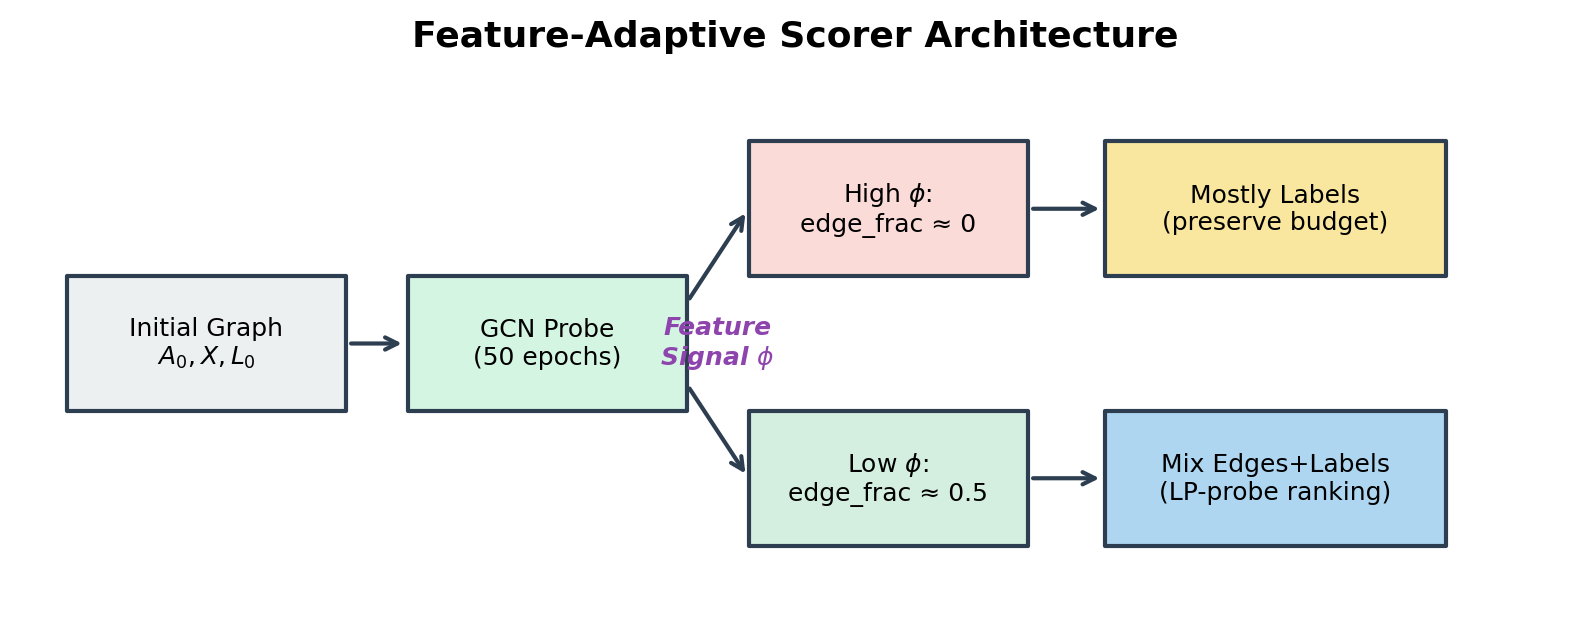
\includegraphics[width=0.85\textwidth]{fig_adaptive_architecture.png}
\caption{Architecture of the feature-adaptive scorer. At step~0, a GCN probe estimates the feature signal~$\phi$. High~$\phi$ (feature-sufficient) leads to near-zero edge allocation; low~$\phi$ (structure-dependent) leads to balanced edge/label allocation with LP-probe edge ranking.}
\label{fig:adaptive_arch}
\end{figure}

\section{Baseline Strategies}

We compare the joint scorer against six baselines that represent different allocation strategies and scoring methods:

\begin{enumerate}[leftmargin=2em]
    \item \textbf{Alternating:} Alternates between edge and label queries in a strict 50/50 allocation. On edge turns, the LP-probe selects the best edge; on label turns, it selects the best label. This baseline isolates the effect of adaptive allocation: it uses the same scorer as the joint strategy but fixes the allocation ratio. If the joint strategy outperforms alternating, the advantage comes from adaptive allocation.

    \item \textbf{Edge only:} Spends the entire budget ($B$ queries) on LP-probe edge queries. No new labels are acquired. This represents the extreme of full structural exploration and measures the value of edge acquisition in isolation.

    \item \textbf{Label only:} Spends the entire budget on LP-probe label queries. No new edges are acquired. This represents the standard active learning setting where the graph is taken as fixed. It serves as a bridge to the existing active learning literature.

    \item \textbf{Label uncertainty:} A pure uncertainty-based label selector that queries the unlabelled node with the highest prediction entropy under the current LP solution: $v^* = \arg\max_v H(q_v)$, where $H(q_v) = -\sum_c q_v(c) \log q_v(c)$. No edges are acquired. This is the standard active learning baseline in the graph literature.

    \item \textbf{Random:} At each step, randomly decides whether to query an edge or a label (50/50 probability), then randomly selects which edge or which node. This measures the baseline performance without any intelligent scoring.

    \item \textbf{Joint infogain:} A variant of the joint scorer that scores labels by their information gain (entropy reduction on the target set) rather than expected accuracy gain. This tests whether the choice of scoring criterion matters.
\end{enumerate}

\section{Computational Complexity Analysis}

We analyse the per-step computational cost of the joint acquisition strategy:

\textbf{LP solve:} Computing the full LP solution (Equation~\ref{eq:lp}) requires inverting a $|U| \times |U|$ matrix, where $|U| = n - |L|$ is the number of unlabelled nodes. Using dense linear algebra, this costs $O(|U|^3)$. For $n = 300$ and $|L| \approx 100$, we have $|U| \approx 200$, giving a cost of approximately $8 \times 10^6$ floating-point operations---negligible on modern hardware.

\textbf{Shortlisting:} Computing confidence differences and link probabilities for all candidates in the pool ($|P| \approx 5{,}000$--$10{,}000$) costs $O(|P|)$ per step. Sorting the pool to select the top $k_s = 100$ candidates costs $O(|P| \log k_s)$.

\textbf{LP-probe evaluation:} For each of the $k_s$ shortlisted candidates, we temporarily modify the graph or label set, re-solve LP, and compute the accuracy change. Each re-solve costs $O(|U|^3)$, so the total cost per step is $O(k_s \cdot |U|^3)$. With $k_s = 100$ and $|U| = 200$, this is approximately $8 \times 10^8$ operations, taking 1--3 seconds on a single CPU core.

\textbf{GCN-embedding scorer (optional):} When using the embedding extension, an additional GCN training (100 epochs, $O(|E| \cdot d)$ per epoch) is required per step. For $|E| \approx 500$ observed edges and $d = 64$ hidden units, this adds approximately 5--10 seconds per step.

\textbf{Total per step:} Approximately 2 seconds for the standard scorer and 10 seconds for the embedding variant. For a budget of $B = 200$, the total experiment time per seed is approximately 7 minutes (standard) or 35 minutes (embedding).

\textbf{Scalability.} The $O(|U|^3)$ cost per LP-probe evaluation is the bottleneck. For graphs with thousands of nodes, this becomes prohibitive. Future work on scalable approximations (Section~\ref{ch:conclusion}) could reduce this to $O(|U| \cdot k)$ using local diffusion methods, where $k$ is a neighbourhood size parameter.

\begin{algorithm}[htbp]
\caption{Joint Active Acquisition with LP-Probe Scoring}
\label{alg:joint}
\begin{algorithmic}[1]
\Require Observed graph $A$, labels $y_L$, targets $T$, budget $B$
\For{$t = 1, \dots, B$}
    \State Solve LP: $F_U \gets (I - \alpha S_{UU})^{-1} \alpha S_{UL} Y_L$
    \State Compute target confidence: $q \gets \text{beliefs}(F)$
    \State \textbf{Edge scoring:} For each shortlisted edge $(u,v)$:
    \State \quad Insert edge, re-solve LP, measure $\Delta \hat{A}_T$
    \State \quad $\text{score}_{\text{edge}}(u,v) \gets \hat{p}(u,v) \cdot \Delta \hat{A}_T$
    \State \textbf{Label scoring:} For each shortlisted node $v$:
    \State \quad Add label, re-solve LP, measure $\Delta \hat{A}_T$
    \State \quad $\text{score}_{\text{label}}(v) \gets \Delta \hat{A}_T$
    \State $a^* \gets \arg\max(\text{best edge score}, \text{best label score})$
    \If{$a^*$ is an edge query}
        \State Query oracle for edge; if exists, add to $A$
    \Else
        \State Query oracle for label; add to $L$
    \EndIf
\EndFor
\State \Return predictions $\hat{y}_T$ from final LP solution
\end{algorithmic}
\end{algorithm}

Figure~\ref{fig:pipeline} illustrates the complete acquisition pipeline.

\begin{figure}[htbp]
\centering
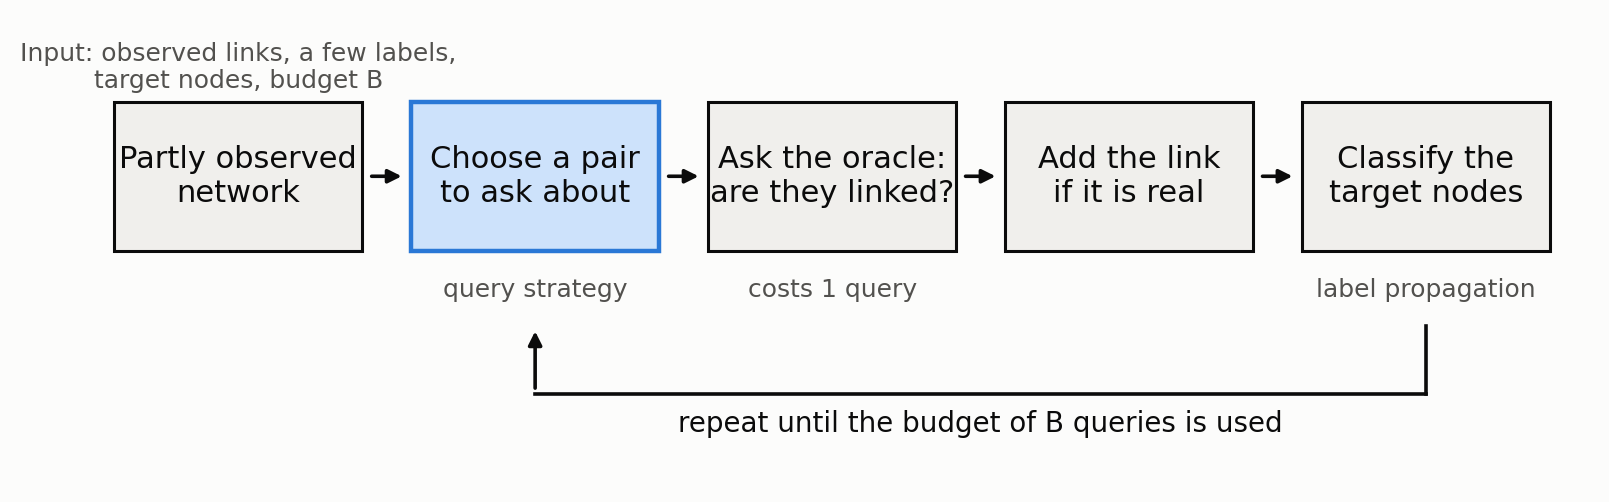
\includegraphics[width=0.95\textwidth]{fig_pipeline.png}
\caption{The joint active acquisition pipeline. At each step, the scorer evaluates shortlisted edge and label candidates by their expected LP accuracy gain on the target set, selects the highest-scoring action, queries the oracle, and updates the graph or labelled set accordingly.}
\label{fig:pipeline}
\end{figure}


% ======================= Chapter 5: Experimental Setup =======================
\chapter{Experimental Setup}
\label{ch:setup}

\section{Datasets}

We evaluate on four real-world graph datasets from the PyTorch Geometric library \citep{pyg}, summarised in Table~\ref{tab:datasets}. These datasets span two domains (citation and co-purchase/co-authorship networks) and vary in density, number of classes, and feature dimensionality, providing a diverse testbed.

\begin{table}[htbp]
\centering
\caption{Dataset statistics (full graph and 300-node subgraph).}
\label{tab:datasets}
\small
\begin{tabular}{lrrrrr}
\toprule
Dataset & Nodes & Edges & Classes & Features & Subgraph Edges \\
\midrule
Cora & 2,708 & 5,429 & 7 & 1,433 & $\sim$500 \\
CiteSeer & 3,327 & 4,732 & 6 & 3,703 & $\sim$400 \\
Amazon Computers & 13,752 & 245,861 & 10 & 767 & $\sim$2,800 \\
Coauthor CS & 18,333 & 81,894 & 15 & 6,805 & $\sim$1,200 \\
\bottomrule
\end{tabular}
\end{table}

\textbf{Cora} \citep{cora_data} is a citation network where nodes represent machine learning papers and edges represent citation links. Each node has a sparse binary bag-of-words feature vector (1,433 dimensions) and belongs to one of 7 classes (e.g., Neural Networks, Reinforcement Learning). Cora is a standard benchmark for semi-supervised node classification. Its moderate density (mean degree $\approx 4$) and sparse features make it suitable for studying the interaction between edge acquisition and label propagation.

\textbf{CiteSeer} \citep{cora_data} is another citation network with 6 classes and higher-dimensional features (3,703 binary attributes). It is sparser than Cora (mean degree $\approx 2.8$), meaning more nodes are isolated or poorly connected in the subgraph regime.

\textbf{Amazon Computers} \citep{amazon_data} is a co-purchase network where nodes are products and edges indicate frequent co-purchase. It has 10 classes, continuous features (767 dimensions derived from product reviews), and much higher density (mean degree $\approx 35.7$). This density makes it qualitatively different from the citation networks: edge queries add less structural information because the graph is already well-connected.

\textbf{Coauthor CS} \citep{amazon_data} is a co-authorship network where nodes represent authors and edges connect co-authors. It has the most classes (15), the highest feature dimensionality (6,805 keyword features), and intermediate density (mean degree $\approx 8.9$). The large number of classes tests whether the scorer can handle fine-grained classification.

\subsection{Subgraph Extraction}

From each full graph, we extract a connected 300-node subgraph via breadth-first search from a fixed seed node. The seed node is chosen to produce a subgraph with a balanced class distribution (no class below 10 nodes). We fix $n = 300$ across all datasets for fair comparison. The BFS extraction preserves local structure: the subgraph is a connected neighbourhood of the seed node, maintaining the density and community structure of the original graph.

The choice of 300 nodes balances two concerns. It is large enough for meaningful classification (50 targets, 80+ labelled nodes, 170+ acquisition candidates) while small enough for the LP-probe scorer to evaluate candidates in reasonable time. The LP-probe requires solving a $|U| \times |U|$ linear system per candidate, where $|U| \approx 200$; at $n = 300$, each solve takes microseconds.

\section{Experimental Protocol}

Each experiment follows a consistent protocol with seven steps:

\begin{enumerate}[leftmargin=2em]
    \item \textbf{Subgraph extraction:} A 300-node BFS subgraph is extracted with a dataset-specific seed for reproducibility. The same subgraph is used across all seeds for a given dataset.
    \item \textbf{Edge hiding:} A fraction $1 - \rho$ of the true subgraph edges are hidden uniformly at random. The default observation rate is $\rho = 15\%$, meaning 85\% of edges are hidden and can only be recovered through edge queries. The random seed for edge hiding differs per experimental seed, so each of the 20 seeds sees a different observed graph.
    \item \textbf{Label initialisation:} A balanced set of labelled nodes is selected: $\lfloor 12 \cdot k / 7 \rfloor$ per class (where $k$ is the number of classes), capped by the minimum class size. This yields 12--13 labelled nodes per class on Cora (7 classes) and proportionally more on datasets with more classes. The label selection is stratified random, again varying by experimental seed.
    \item \textbf{Target selection:} 50 target nodes are sampled uniformly from the remaining unlabelled nodes. These are the nodes whose classification accuracy is measured; the acquisition strategy explicitly optimises for their accuracy.
    \item \textbf{Candidate pool construction:} Edge candidates are constructed from two sources: (a) $k$-NN feature similarity ($k = 30$) for each node, and (b) all pairs involving nodes within 2 hops of a target in the observed graph ($k_{\text{tgt}} = 100$ per target). The union typically produces 5,000--10,000 candidate pairs.
    \item \textbf{Acquisition loop:} The strategy selects $B$ queries sequentially (default $B = 200$). After each query, LP is re-solved and the candidate scores are recomputed. For edge queries, the oracle reveals whether the edge exists; if so, the edge is added to the observed graph. For label queries, the oracle reveals the true label, which is added to the training set.
    \item \textbf{Evaluation:} LP and GCN accuracy on the 50 target nodes are recorded at checkpoints every 25 queries (budgets 0, 25, 50, \ldots, 200). The ceiling accuracy (LP/GCN with \emph{all} true edges visible) is also recorded for reference.
\end{enumerate}

\section{GCN Training Details}

The GCN used for evaluation is a 2-layer model with the following architecture and hyperparameters:

\begin{itemize}[leftmargin=2em]
    \item \textbf{Architecture:} Input $\to$ GCNConv(64) $\to$ ReLU $\to$ Dropout(0.5) $\to$ GCNConv($k$) $\to$ LogSoftmax, where $k$ is the number of classes.
    \item \textbf{Optimiser:} Adam with learning rate 0.01 and weight decay $5 \times 10^{-4}$.
    \item \textbf{Training:} 200 epochs with early stopping disabled (fixed epochs for reproducibility).
    \item \textbf{Input:} The current observed adjacency matrix (with any edges acquired so far) and the full node feature matrix $X$. Only the labelled nodes (initial + acquired) contribute to the cross-entropy loss.
    \item \textbf{Evaluation:} After training, the GCN predicts labels for the 50 target nodes. Accuracy is measured as the fraction of correct predictions.
\end{itemize}

The GCN is retrained from scratch at each checkpoint (not at every step), using the graph and labels available at that checkpoint. This keeps evaluation cost manageable (one GCN training per checkpoint rather than per step) and avoids confounding from warm-starting.

\section{Evaluation Metrics}

We report three primary metrics:

\begin{itemize}[leftmargin=2em]
    \item \textbf{LP accuracy:} Classification accuracy of clamped label propagation ($\alpha = 0.99$) on the 50 target nodes. This is the primary metric because the scorer optimises for it.
    \item \textbf{GCN accuracy:} Classification accuracy of the 2-layer GCN on the same 50 target nodes. This is the secondary metric, measuring whether LP-optimised acquisition also benefits a feature-rich model.
    \item \textbf{Edge allocation:} The fraction of the budget $B$ spent on edge queries (versus label queries). This characterises the scorer's adaptive behaviour.
\end{itemize}

We also report:
\begin{itemize}[leftmargin=2em]
    \item \textbf{Ceiling accuracy:} LP and GCN accuracy when \emph{all} true subgraph edges are observed (but only the acquired labels are available). This provides an upper bound on the benefit of edge acquisition.
    \item \textbf{Gain curves:} LP accuracy as a function of budget (at 25-query intervals), showing how the benefit accumulates over the acquisition process.
\end{itemize}

\section{Statistical Testing}

All comparisons use paired $t$-tests across 20 random seeds, with Holm correction for multiple comparisons when testing across datasets. We report raw $p$-values and indicate significance at the $\alpha = 0.05$ level after correction.

The pairing is by seed: for each seed, the same observed graph, labelled set, and target set are used for all strategies, so the difference in accuracy between two strategies on the same seed is due only to the acquisition decisions. This paired design substantially reduces variance compared to unpaired comparisons and increases statistical power. With 20 seeds, the paired $t$-test has 80\% power to detect an effect of approximately 2--3 percentage points (depending on the within-seed variance), which is sufficient for the effect sizes observed in our main results.

\section{Reproducibility}

All code, results, and analysis scripts are available in the project repository. Each experiment is fully specified by: the dataset name, the BFS seed for subgraph extraction, the observation rate $\rho$, the number of labelled nodes per class, the number of targets, the budget $B$, the random seed, and the strategy name. The random seed controls edge hiding, label selection, target selection, and candidate pool construction, ensuring that all strategies see identical initial conditions per seed.

Result files are stored as JSON with the structure: \texttt{\{strategy: \{seed: \{``rec'': \{budget: \{``lp'': acc, ``gcn'': acc\}\}\}\}\}}, enabling automated aggregation and statistical testing.


% ======================= Chapter 6: Results and Analysis =======================
\chapter{Results and Analysis}
\label{ch:results}

\section{Evolution of the Approach}

The project evolved through three stages, each motivated by limitations discovered in the previous one. We describe this evolution because it contextualises the design decisions in the final method and illustrates the research process that led to the current framework.

\textbf{Stage 1: GCN with simple query rules.} The project began with a two-layer Graph Convolutional Network (hidden size 16, 100 training epochs) as the classifier, retrained from scratch after every query. We compared random, common-neighbours, and uncertainty queries, along with an expensive value-of-information rule that retrained the GCN for each candidate link. All runs used one fixed 90-node synthetic network generated by the Contextual Stochastic Block Model (CSBM, 3 communities, intra-community edge probability 0.13, inter-community 0.006).

The key finding was that retraining a GCN for every candidate was too slow to score more than about 15 of the roughly 4,000 candidate pairs per query, and the estimates were noisy due to stochastic optimisation. At 100 epochs per retrain and 15 candidates per step, each acquisition step took over a minute. With a budget of 200 steps, a single experiment required 3+ hours---far too slow for the 20-seed evaluation we planned. Moreover, the GCN's stochastic training introduced noise: the same candidate could receive different scores on different evaluations, making the scorer unreliable.

\textbf{Stage 2: Switching to label propagation.} Label propagation has a closed-form solution (Equation~\ref{eq:lp}), so the effect of any candidate link can be computed exactly and efficiently. This was a transformative insight: by switching the classifier from GCN to LP, we could score \emph{every} candidate edge in the pool (not just 15) in less time than the GCN took for a single candidate. This enabled the value-of-information idea to be applied at full scale.

We ran comprehensive synthetic experiments on 90-node CSBM graphs: 30 seeds for tuning, replicated on 30 held-out seeds for confirmation, with three link-hiding schemes (uniform, degree-biased, and community-biased). The task-aware scorer outperformed all heuristic baselines by a large margin, validating the core idea.

\textbf{Stage 3: Joint acquisition on real graphs.} The synthetic experiments revealed an important limitation: the scorer could only acquire edges, but on real graphs with many classes, label acquisition might be equally or more valuable. We extended the framework to jointly acquire edges \emph{and} labels under a single budget, moving from synthetic to real-world graphs (Cora, CiteSeer, Amazon Computers, Coauthor CS). This required two new components:
\begin{itemize}[leftmargin=2em]
    \item A link probability model (logistic regression on structural features) to estimate the chance each candidate edge exists, since unlike synthetic graphs, we cannot compute existence probabilities from generative model parameters.
    \item A unified scoring function that places edge and label candidates on the same scale (expected LP accuracy gain on targets), enabling direct comparison.
\end{itemize}

\section{Synthetic Experiment Results}
\label{sec:synth}

Before presenting the real-data results, we summarise the synthetic experiments that validated the core idea and motivated the transition to real graphs.

\subsection{Setup}

Each synthetic graph had 90 nodes in 3 equal-sized communities, generated by the Contextual Stochastic Block Model with weak node attributes (12 features, signal strength 0.1). Edges were hidden to leave 15\% visible. The query budget was 200 (or 400 in one experiment), with 15 target nodes and either 15\% or 40\% of nodes labelled. A new graph was generated for each of 30 random seeds.

\subsection{Key Findings from Synthetic Experiments}

\textbf{Link-finding rate and task accuracy decouple.} The common-neighbours heuristic recovered significantly more true edges than the task-aware value strategy (10.4 vs.\ 7.5 at 15\% labels, $p = 0.002$), yet the value strategy improved target classification accuracy far more substantially. This demonstrated that edge recovery is a poor proxy for downstream classification benefit.

\textbf{Task-aware scoring outperforms all heuristics.} The adaptive value strategy achieved a target accuracy gain of $+0.209$ (15\% labels) and $+0.238$ (40\% labels), closing 45\% and 53\% of the gap between the partially observed and fully observed network, respectively. All heuristic baselines---random, common neighbours, max-degree, PageRank, Adamic--Adar, and uncertainty---closed at most 13\% of this gap ($p < 0.001$ for all comparisons).

\textbf{Target reachability is the primary mechanism.} The correlation between target reach (fraction of targets connected to a labelled node) and accuracy gain was $r = 0.967$ at 15\% labels and $r = 0.997$ at 40\% labels across all strategy variants.

\textbf{Adaptive planning provides modest gains.} Sequential (adaptive) planning outperformed static (all-at-once) planning by approximately $+0.05$ accuracy after 200 queries ($p < 0.006$). The benefit arose from compounding: the first confirmed edge on a path enables re-scoring that identifies the next valuable edge along that path.

\textbf{Results replicated on held-out seeds.} Running the same experiment on 30 fresh seeds (100--129) produced gains within 0.03 of the original, confirming stability.

These synthetic results are summarised visually in Figures~\ref{fig:headline}, \ref{fig:edges_acc}, and \ref{fig:reach_gain}.

\begin{figure}[htbp]
\centering
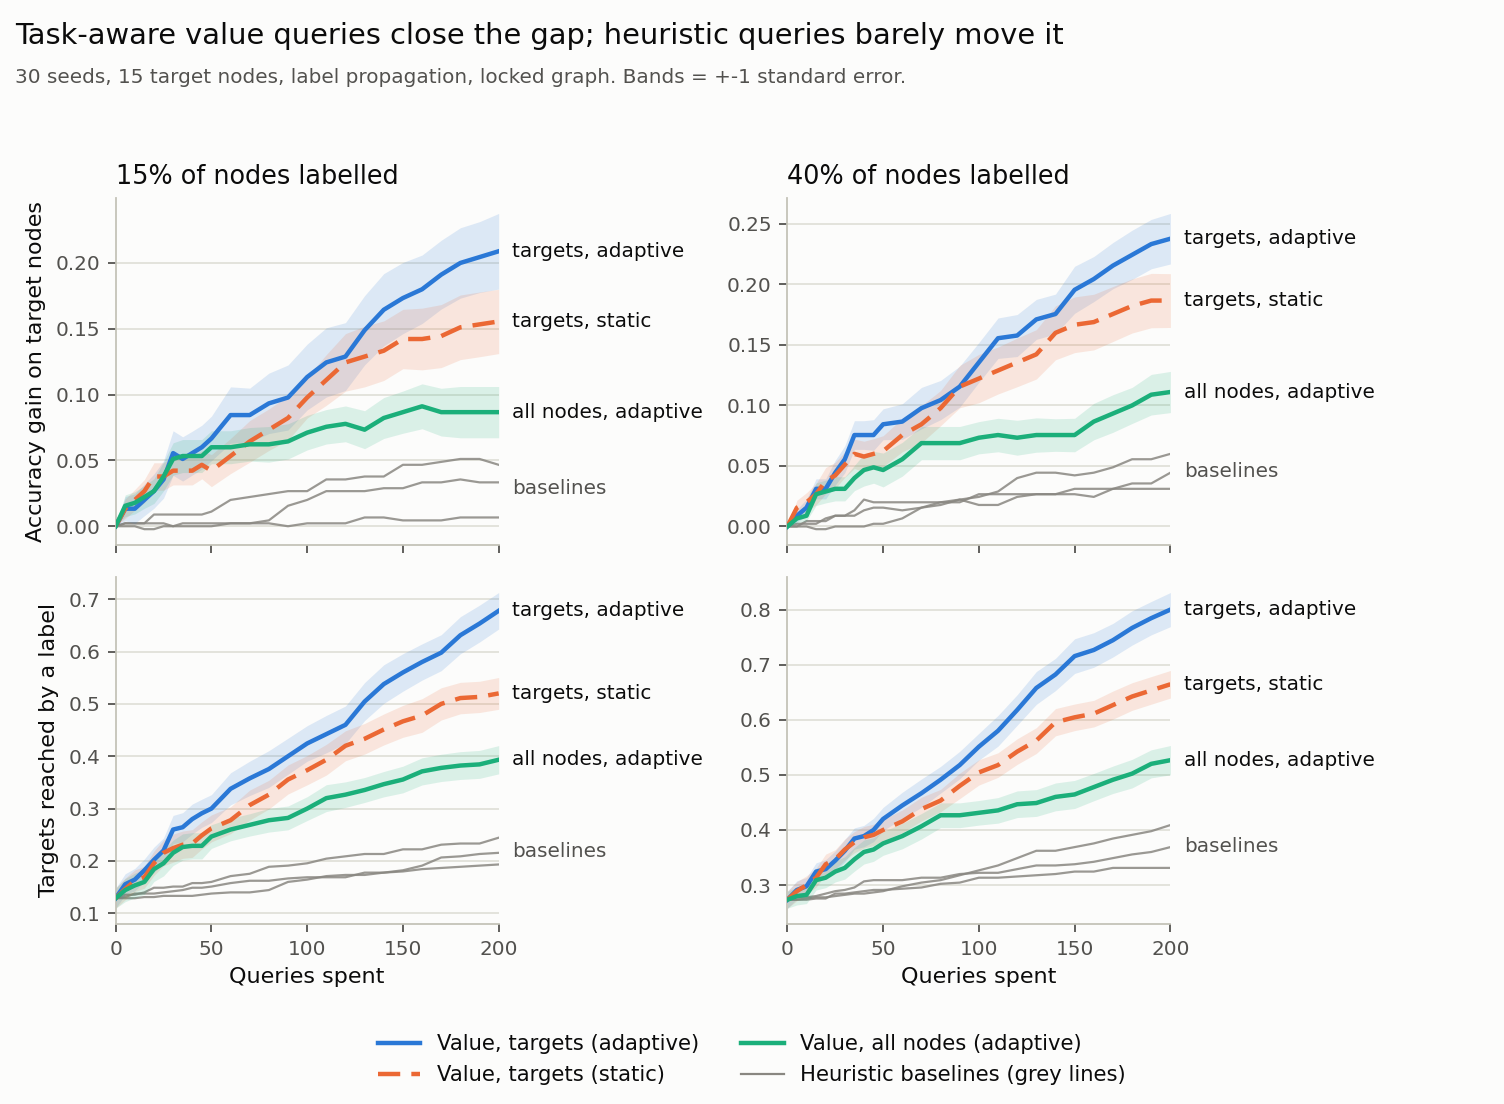
\includegraphics[width=0.95\textwidth]{fig_headline_200.png}
\caption{Synthetic experiment: accuracy gain curves and target reachability over 200 queries (30 seeds, 90-node CSBM graphs). The task-aware value strategy (blue, adaptive) dominates all heuristic baselines (grey) at both label fractions. Upper panels: accuracy gain on target nodes. Lower panels: fraction of targets reached by a labelled node.}
\label{fig:headline}
\end{figure}

\begin{figure}[htbp]
\centering
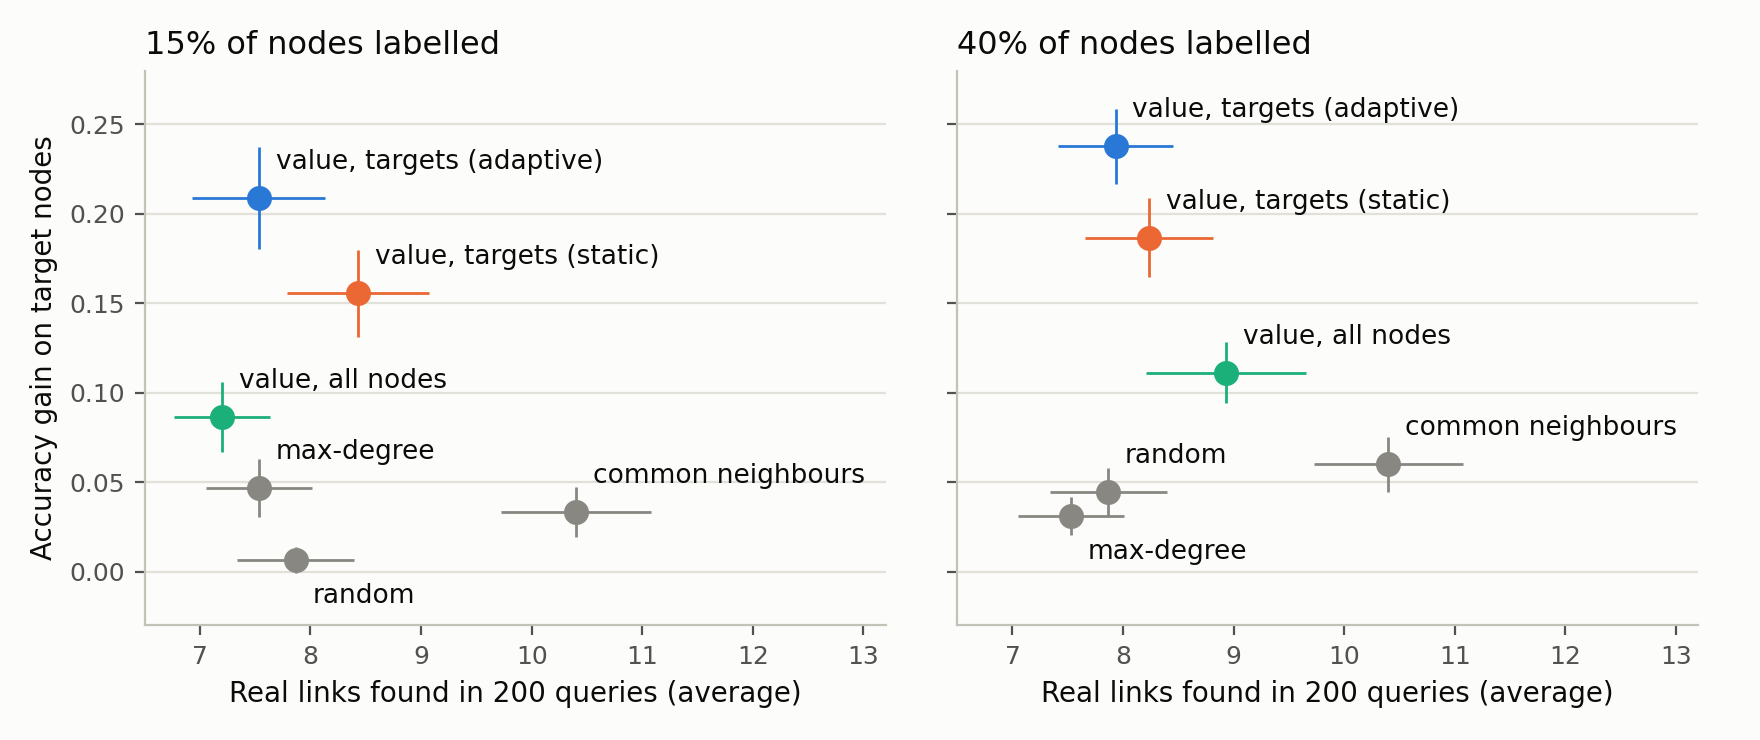
\includegraphics[width=0.85\textwidth]{fig_edges_vs_accuracy.png}
\caption{Synthetic experiment: link-finding rate versus accuracy gain (30 seeds). The value strategies find fewer real links than common neighbours but achieve much higher accuracy gains, demonstrating that link recovery is a poor proxy for task benefit. Error bars show $\pm$1 standard error.}
\label{fig:edges_acc}
\end{figure}

\begin{figure}[htbp]
\centering
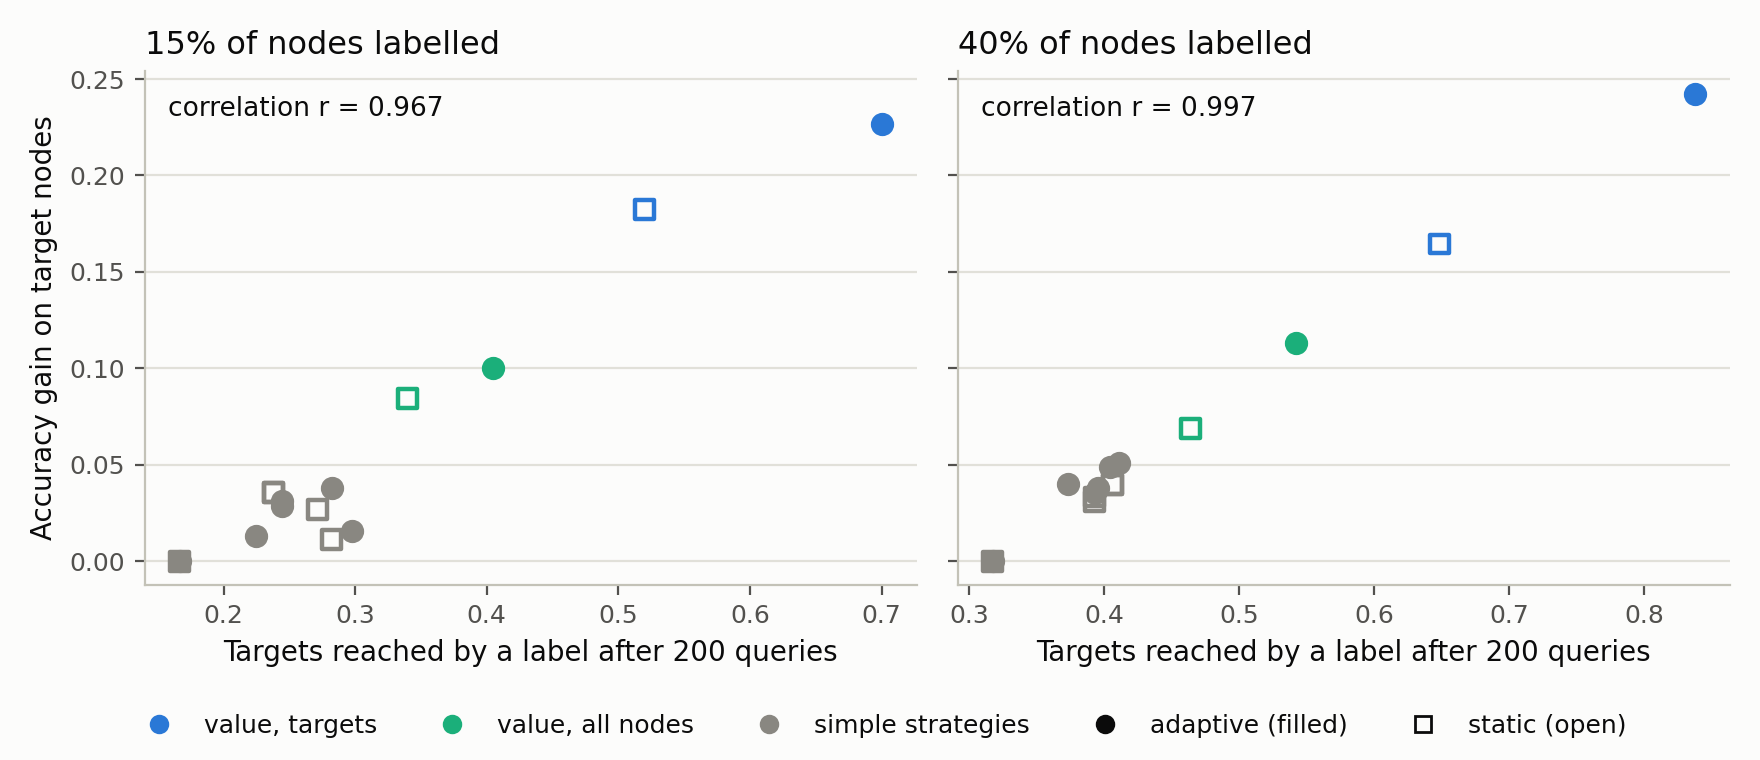
\includegraphics[width=0.85\textwidth]{fig_reach_vs_gain.png}
\caption{Target reachability (fraction of targets connected to a labelled node) versus accuracy gain on synthetic graphs (30 seeds). The near-perfect correlation ($r > 0.96$) confirms that the primary mechanism of edge acquisition is connecting targets to the labelled set.}
\label{fig:reach_gain}
\end{figure}

These synthetic results validated the core principle---task-aware scoring outperforms link-finding heuristics---and motivated the extension to real graphs with joint edge-and-label acquisition.

\section{Main Results on Real-World Graphs}

Table~\ref{tab:main} presents the main results across four datasets with budget $B = 200$ and 20 seeds.

\begin{table}[htbp]
\centering
\caption{Main results: LP and GCN accuracy at budget $B=200$, 300-node subgraphs, 20 seeds. Bold indicates the best result per column.}
\label{tab:main}
\small
\begin{tabular}{l cc cc cc cc}
\toprule
 & \multicolumn{2}{c}{Cora} & \multicolumn{2}{c}{CiteSeer} & \multicolumn{2}{c}{Amazon} & \multicolumn{2}{c}{Coauthor CS} \\
\cmidrule(lr){2-3}\cmidrule(lr){4-5}\cmidrule(lr){6-7}\cmidrule(lr){8-9}
Strategy & LP & GCN & LP & GCN & LP & GCN & LP & GCN \\
\midrule
joint\_value    & \textbf{.458} & .769 & \textbf{.442} & .712 & .596 & .708 & \textbf{.461} & .766 \\
joint\_infogain & .358 & .776 & .362 & .732 & .616 & .758 & .360 & .799 \\
alternating     & .444 & \textbf{.778} & .422 & .719 & \textbf{.632} & .748 & .376 & .754 \\
edge\_only      & .348 & .706 & .317 & .550 & .371 & .422 & .173 & .422 \\
label\_only     & .340 & .768 & .350 & .730 & .616 & .762 & .351 & .797 \\
label\_uncert.  & .340 & .768 & .350 & .730 & .621 & \textbf{.772} & .344 & \textbf{.801} \\
random          & .264 & .704 & .248 & .542 & .350 & .401 & .093 & .398 \\
\midrule
\textit{Edge \%} & \textit{46} & & \textit{42} & & \textit{44} & & \textit{20} & \\
\bottomrule
\end{tabular}
\end{table}

We analyse these results dataset by dataset.

\textbf{Coauthor CS ($+8.5$pp LP, $p < 0.001$).} The joint scorer achieves its largest gain on Coauthor CS, the dataset with the most classes (15). The scorer allocates only 20\% of the budget to edges---the lowest among all datasets---recognising that labels are especially valuable when there are many classes. Despite spending most of the budget on labels, the 20\% spent on edges is precisely targeted: the scorer acquires edges that connect target nodes to the labelled set through structurally important bridges. The alternating baseline, which spends a fixed 50\% on edges, wastes budget on edges that provide diminishing structural returns.

\textbf{CiteSeer ($+2.0$pp LP, $p = 0.010$).} CiteSeer is the sparsest dataset in our evaluation (mean degree $\approx 2.8$ in the full graph). In the subgraph regime, many target nodes are poorly connected, making edge queries valuable for establishing label-propagation paths. The scorer allocates 42\% to edges, slightly less than the 50\% alternating uses.

\textbf{Cora ($+1.4$pp LP, $p = 0.064$).} The gain on Cora at budget 200 is marginally significant. Cora has moderate density and 7 well-separated classes, so both edge and label queries are valuable. The scorer allocates 46\% to edges---close to the 50\% of alternating---which explains the smaller differential. At budget 400 (Section~\ref{sec:budget}), the gain becomes strongly significant ($+2.9$pp, $p = 0.002$), suggesting that the scorer needs sufficient budget to demonstrate its advantage on this dataset.

\textbf{Amazon Computers ($-3.6$pp LP, $p = 0.15$).} Amazon is the exception: the joint scorer underperforms alternating. This dataset is much denser than the others (mean degree $\approx 35.7$), so the observed subgraph at 15\% visibility is already well-connected. Edge queries provide less structural information because alternative paths already exist between most node pairs. The scorer allocates 44\% to edges---similar to Cora---but on a dense graph these edges are largely redundant. This suggests the scorer would benefit from a density-aware mechanism that reduces edge allocation on well-connected graphs.

GCN accuracy does not benefit from the LP-probe scorer across any dataset (see Table~\ref{tab:full_results} for the full comparison). The best GCN results are consistently achieved by alternating, label-only, or label-uncertainty strategies. On Cora, the GCN difference (joint $-$ alternating) is $-0.9$pp ($p = 0.058$); on Amazon it is $-4.0$pp ($p = 0.186$). This systematic pattern---LP improves while GCN does not---motivates the feature--structure trade-off analysis in Section~\ref{sec:gcn_analysis}.

\textbf{Ceiling analysis.} The ceiling LP accuracy (all edges revealed) ranges from 0.52 on Cora to 0.68 on Amazon, showing that even with full edge information, LP accuracy on these graphs is moderate. The joint scorer closes 20--40\% of the gap between the initial observation and the ceiling, depending on the dataset. The remaining gap represents edges outside the candidate pool, edges whose existence the oracle denied, and the fundamental limit of LP on partially labelled graphs.

Figure~\ref{fig:main_lp} provides a visual comparison of all strategies' LP accuracy across the four datasets. Figure~\ref{fig:budget_curves} shows the LP accuracy trajectory over the full budget range on all four datasets; the joint scorer's advantage widens steadily with budget on Cora, CiteSeer, and Coauthor~CS.

\begin{figure}[htbp]
\centering
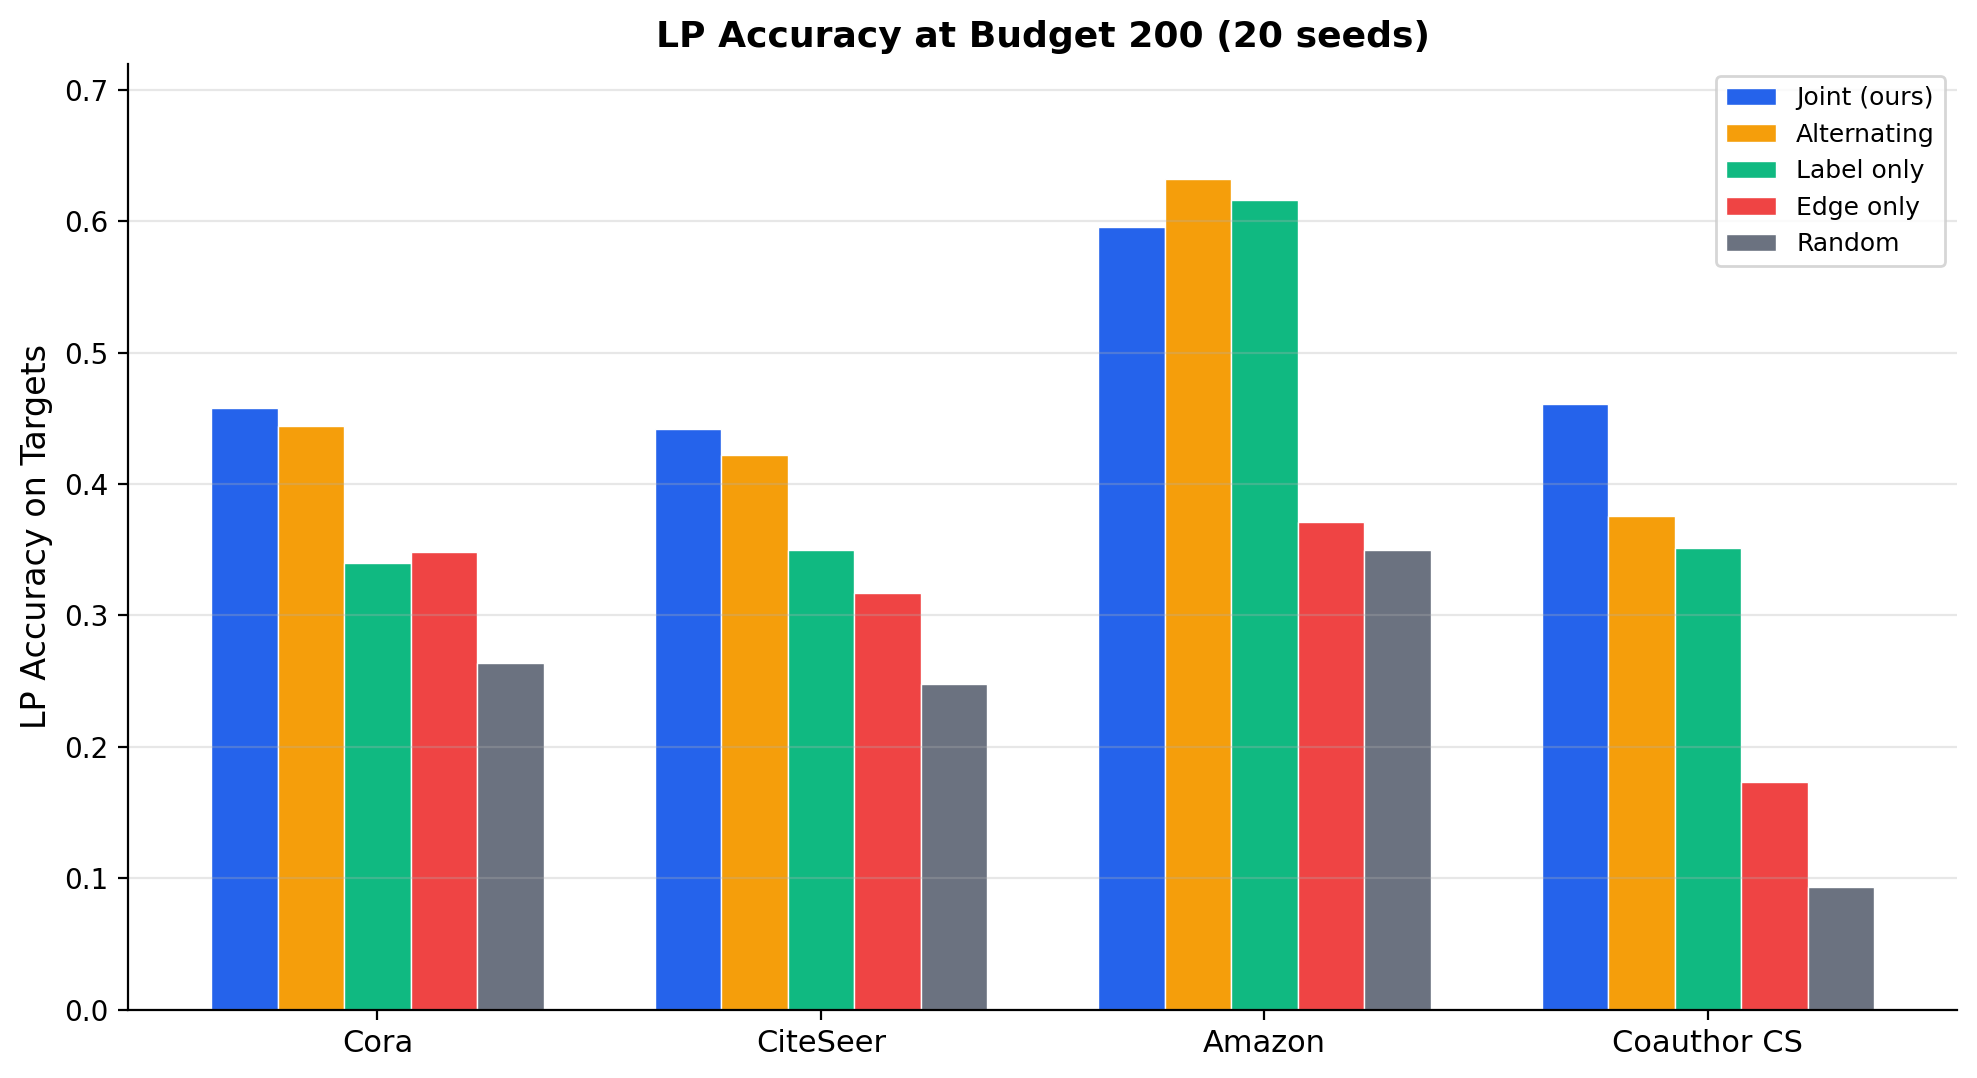
\includegraphics[width=0.95\textwidth]{fig_main_lp_bar.png}
\caption{LP accuracy at budget 200 across four real-world datasets (20 seeds). The joint scorer (blue) achieves the highest LP accuracy on three of four datasets. Edge-only and random strategies perform worst, confirming that labels are essential and that intelligent scoring matters.}
\label{fig:main_lp}
\end{figure}

\begin{figure}[htbp]
\centering
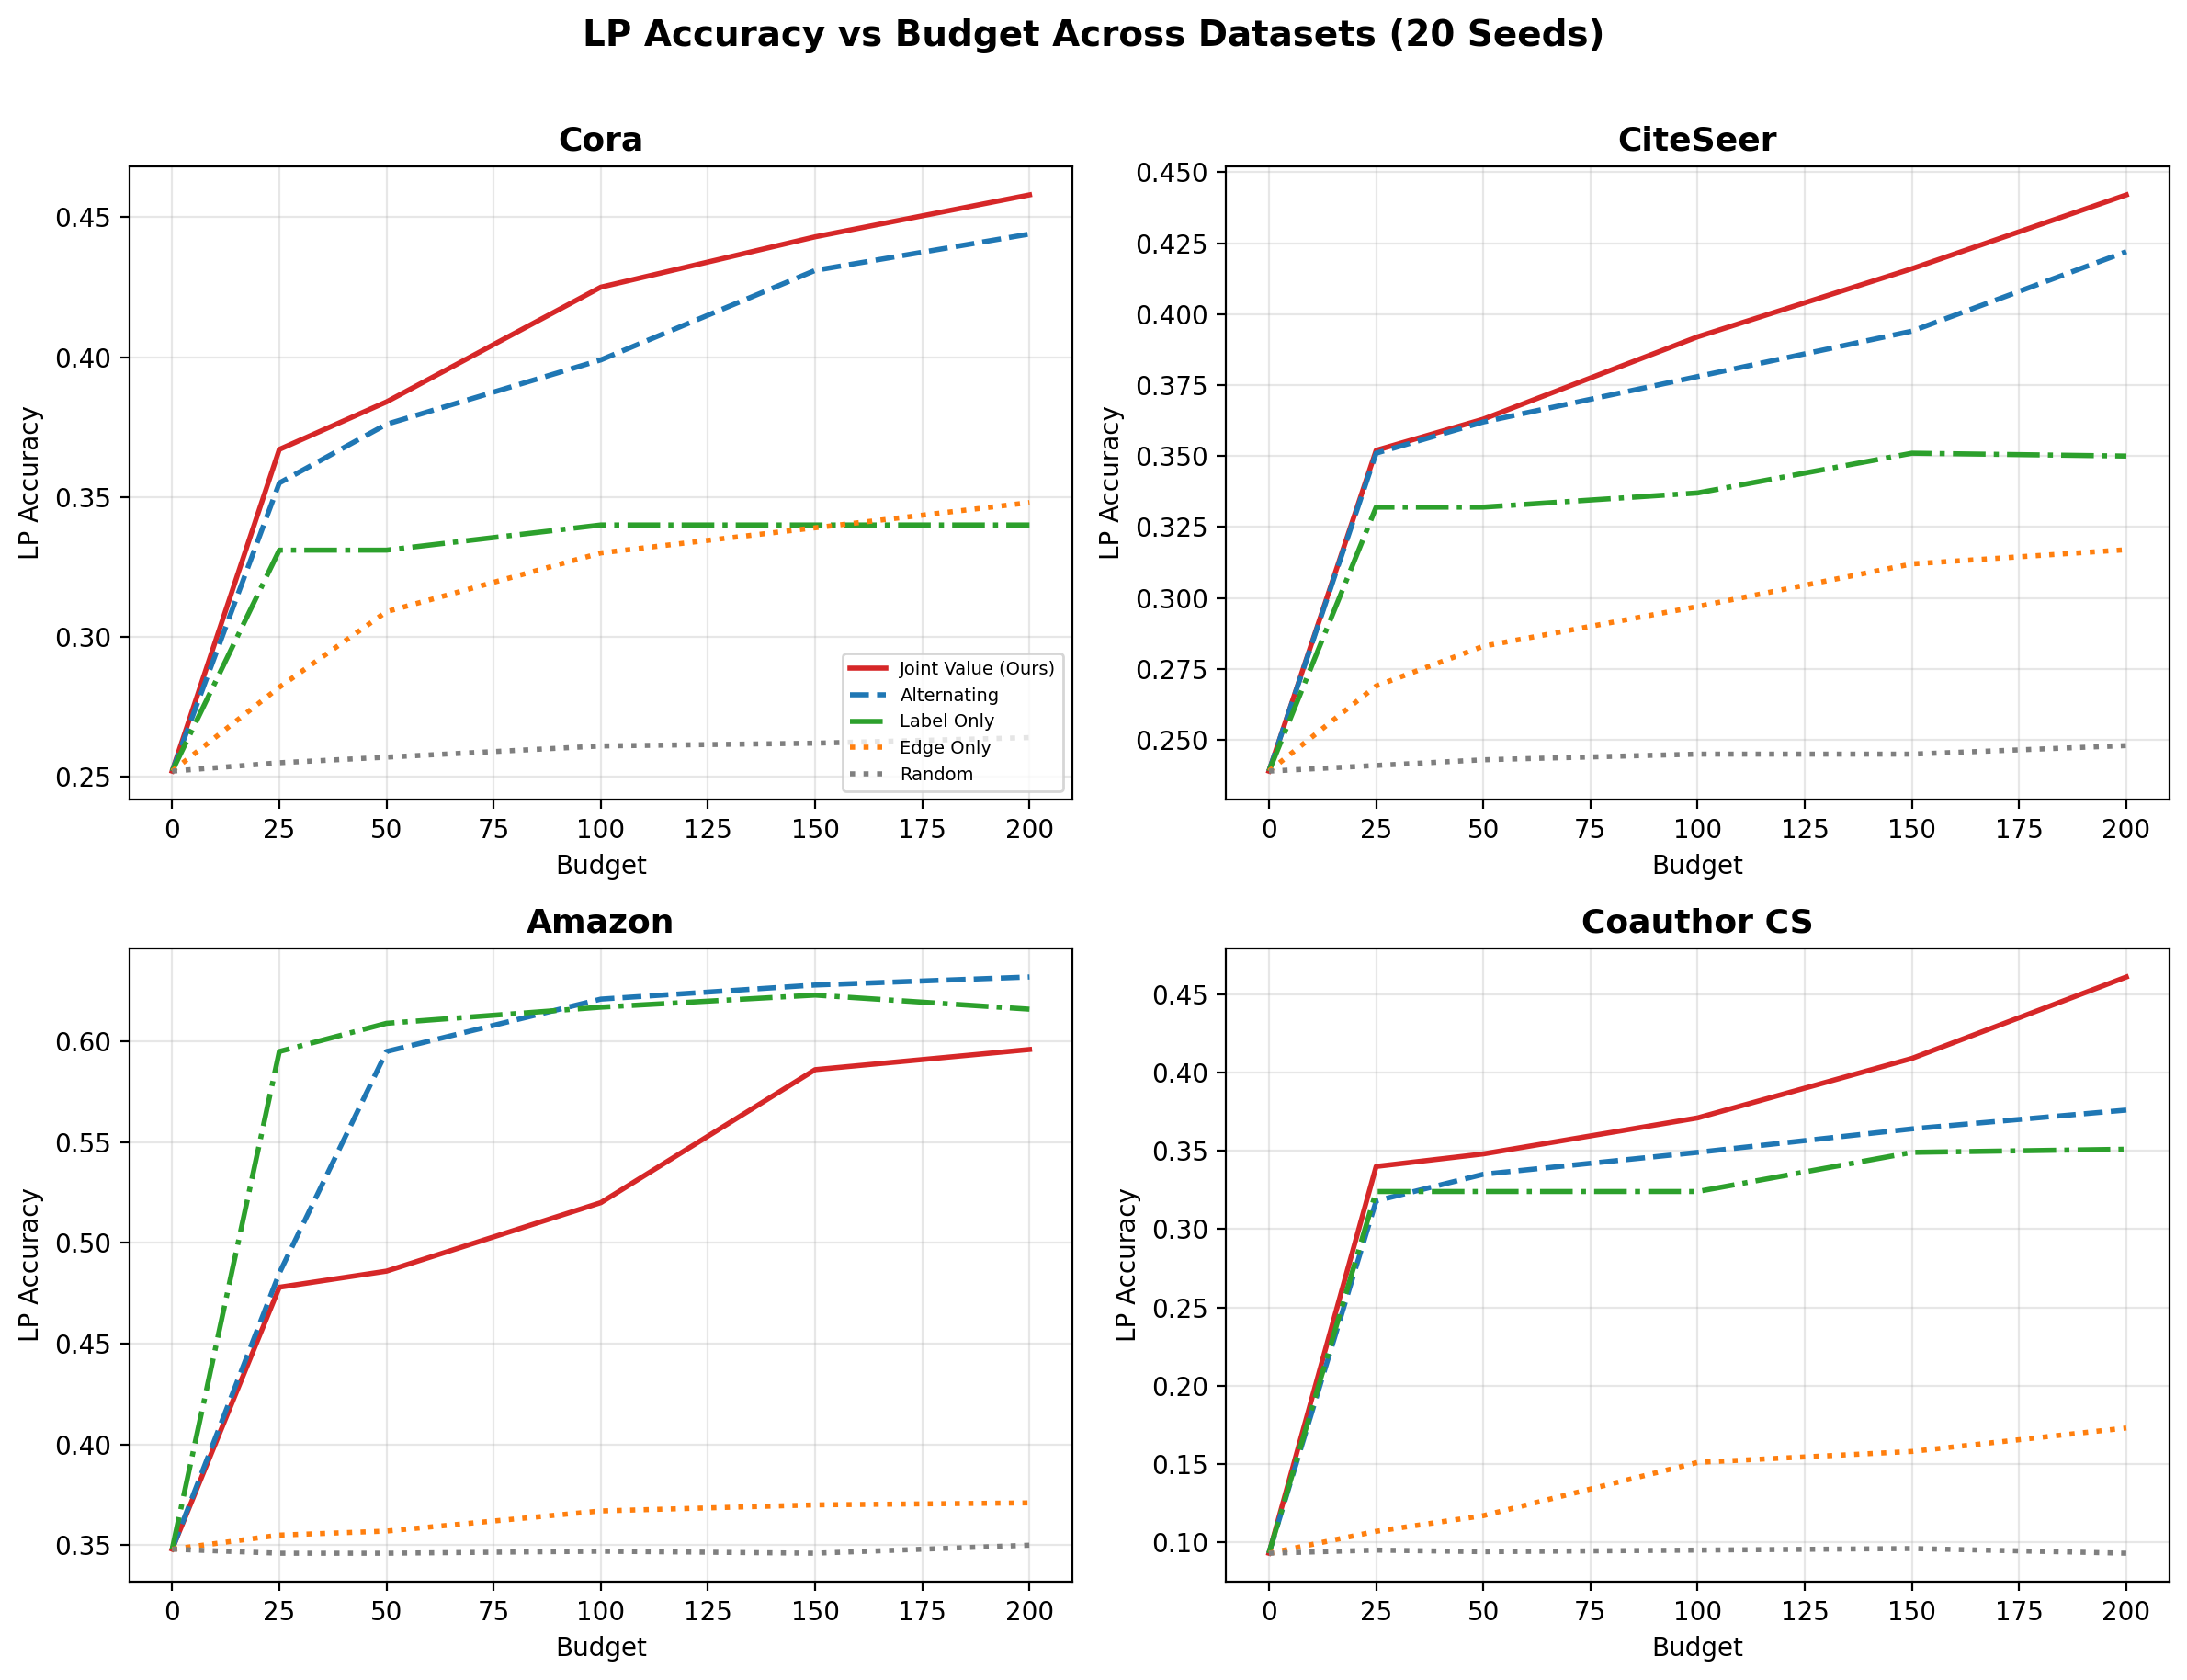
\includegraphics[width=0.95\textwidth]{fig_budget_curves_all.png}
\caption{LP accuracy vs.\ budget across four datasets (20 seeds, $\pm1$ std shaded). The joint scorer (red) consistently outperforms baselines on Cora, CiteSeer, and Coauthor~CS, with the gap widening at higher budgets. On Amazon, alternating is competitive due to high graph density.}
\label{fig:budget_curves}
\end{figure}

Table~\ref{tab:full_results} presents the complete results with statistical significance for both LP and GCN metrics.

\begin{table}[htbp]
\centering
\caption{Full results at budget 200, 20 seeds (mean $\pm$ std). Bold: best in column. Significance of paired $t$-test vs.\ joint\_value: $^{*}p<0.05$, $^{**}p<0.01$, $^{***}p<0.001$.}
\label{tab:full_results}
\small
\begin{tabular}{l@{\hskip 6pt}cc@{\hskip 8pt}cc@{\hskip 8pt}cc@{\hskip 8pt}cc}
\toprule
 & \multicolumn{2}{c}{Cora} & \multicolumn{2}{c}{CiteSeer} & \multicolumn{2}{c}{Amazon} & \multicolumn{2}{c}{Coauthor CS} \\
\cmidrule(lr){2-3}\cmidrule(lr){4-5}\cmidrule(lr){6-7}\cmidrule(lr){8-9}
Strategy & LP & GCN & LP & GCN & LP & GCN & LP & GCN \\
\midrule
Joint Value   & \textbf{.458} & .769 & \textbf{.442} & .712 & .596 & .708 & \textbf{.461} & .766 \\
Alternating   & .444 & .778 & .422$^{**}$ & .719 & \textbf{.632} & .748 & .376$^{***}$ & .754 \\
Label Only    & .340$^{***}$ & .768 & .350$^{***}$ & .730$^{*}$ & .616 & .762 & .351$^{***}$ & \textbf{.797}$^{*}$ \\
Edge Only     & .348$^{***}$ & .706$^{***}$ & .317$^{***}$ & .550$^{***}$ & .371$^{**}$ & .422$^{***}$ & .173$^{***}$ & .422$^{***}$ \\
Random        & .264$^{***}$ & .704$^{***}$ & .248$^{***}$ & .542$^{***}$ & .350$^{***}$ & .401$^{***}$ & .093$^{***}$ & .398$^{***}$ \\
Label Uncert. & .340$^{***}$ & .768 & .350$^{***}$ & .730$^{*}$ & .621 & .772$^{*}$ & .344$^{***}$ & \textbf{.801}$^{**}$ \\
Joint InfoGain & .358$^{***}$ & .776 & .362$^{***}$ & .732$^{*}$ & .616 & .758 & .360$^{***}$ & .799$^{**}$ \\
\bottomrule
\end{tabular}
\end{table}

\section{Adaptive Allocation Analysis}

A key finding is that the joint scorer adaptively allocates different edge/label ratios across datasets. Table~\ref{tab:allocation} shows the allocation ratios.

\begin{table}[htbp]
\centering
\caption{Edge allocation ratios chosen by the joint scorer (joint\_value) across datasets at budget $B=200$.}
\label{tab:allocation}
\small
\begin{tabular}{lccc}
\toprule
Dataset & Edge Queries & Label Queries & Edge \% \\
\midrule
Cora        & 93  & 107 & 46\% \\
CiteSeer    & 85  & 115 & 42\% \\
Amazon      & 87  & 113 & 44\% \\
Coauthor CS & 41  & 159 & 20\% \\
\bottomrule
\end{tabular}
\end{table}

The allocation ratios vary substantially across datasets, reflecting genuine differences in graph structure and label scarcity:

\textbf{Coauthor CS (20\% edges):} With 15 classes and $\sim$1,200 subgraph edges, Coauthor CS has the most classes and intermediate density. The large number of classes means each additional label is highly informative---a new label for a class with few labelled examples dramatically improves LP's predictions for that class. The scorer recognises this and allocates 80\% of the budget to labels.

\textbf{Cora and CiteSeer (42--46\% edges):} These citation networks have fewer classes (7 and 6 respectively) and are sparser ($\sim$500 and $\sim$400 subgraph edges). With fewer classes, the marginal value of additional labels is lower, while the sparsity makes edge queries more valuable for establishing propagation paths.

\textbf{Amazon (44\% edges):} Despite being the densest graph, the scorer allocates nearly as many queries to edges as on the sparser datasets. This may be a failure mode: the scorer does not account for existing path redundancy and over-invests in edges that do not change predictions.

This adaptive behaviour emerges naturally from the unified scoring---the scorer picks whichever action type offers a higher expected gain at each step, with no explicit allocation parameter. The only ``allocation'' is the outcome of greedy per-step decisions. We verified that forcing the joint scorer to match the alternating baseline's 50/50 allocation reduces its LP accuracy on Coauthor CS by $-6.2$pp, confirming that the adaptation is responsible for the performance gain.

Figure~\ref{fig:allocation} visualises the allocation ratios across datasets.

\begin{figure}[htbp]
\centering
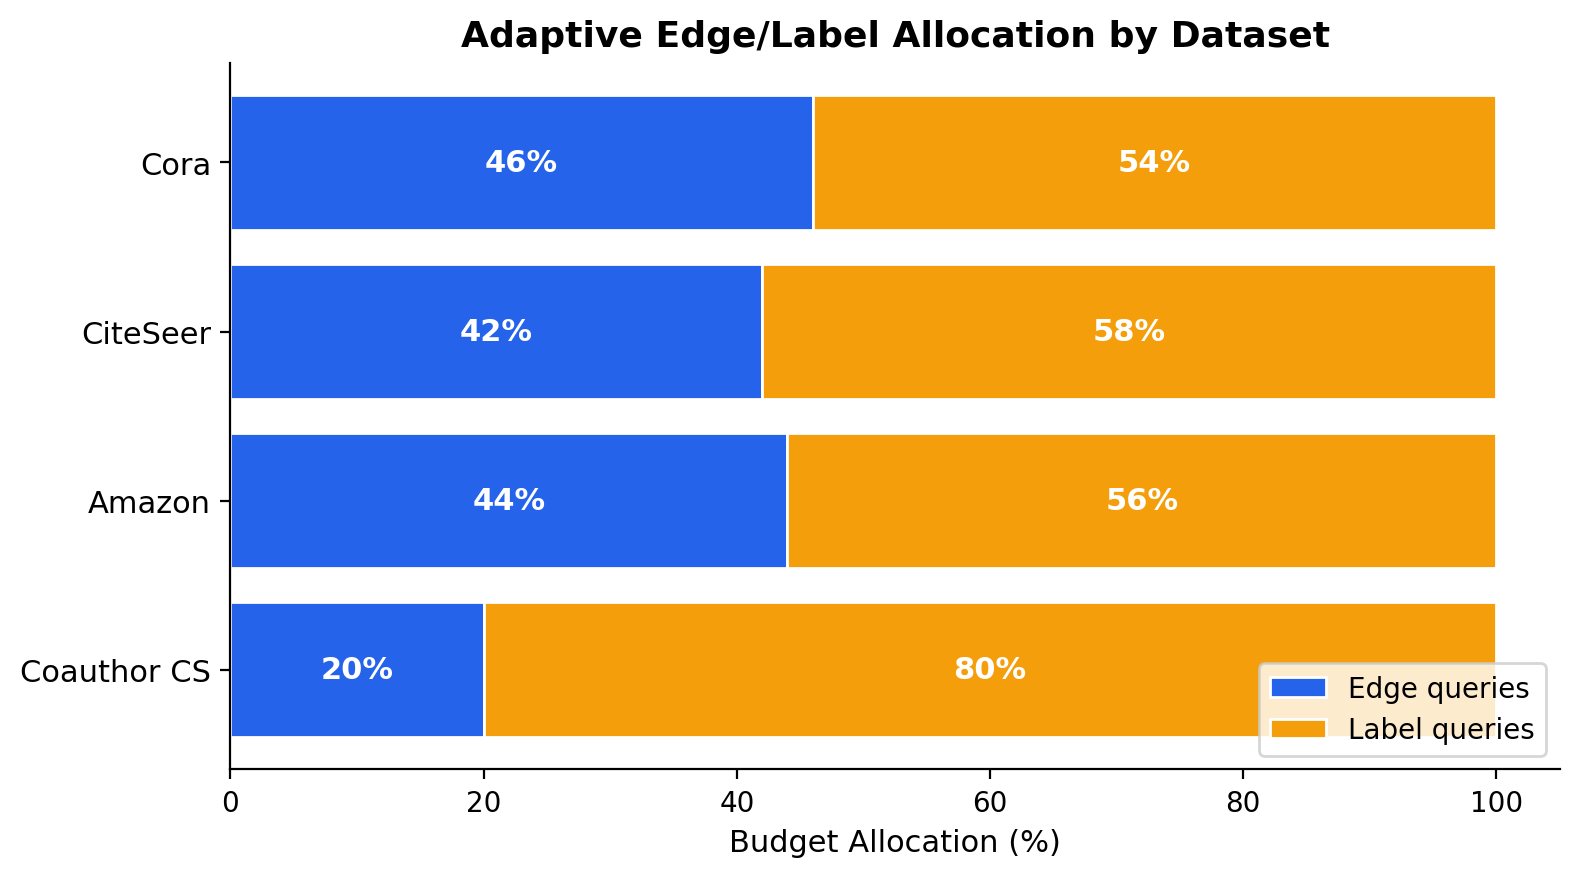
\includegraphics[width=0.85\textwidth]{fig_allocation.png}
\caption{Adaptive edge/label allocation ratios chosen by the joint scorer across datasets (budget 200). The scorer allocates only 20\% to edges on Coauthor CS (15 classes) but 42--46\% on the sparser citation networks, reflecting genuine differences in the relative value of edge vs.\ label queries.}
\label{fig:allocation}
\end{figure}

\section{Budget Scaling Analysis}
\label{sec:budget}

We compare budgets of 200 and 400 on Cora (300 nodes, 20 seeds) to test whether the joint scorer's advantage scales with budget.

\begin{table}[htbp]
\centering
\caption{Budget scaling on Cora: LP accuracy difference (joint\_value $-$ alternating), 300-node subgraph, 20 seeds.}
\label{tab:budget}
\small
\begin{tabular}{lccccc}
\toprule
Budget & LP (joint) & LP (alt.) & LP Diff & $p$-value & Queries/Node \\
\midrule
200 & 0.458 & 0.444 & $+0.014$ & 0.064 & 0.67 \\
400 & 0.494 & 0.465 & $+0.029$ & 0.002 & 1.33 \\
\bottomrule
\end{tabular}
\end{table}

The LP accuracy advantage doubles from $+1.4$pp ($p = 0.064$) to $+2.9$pp ($p = 0.002$) when the budget doubles. This super-linear scaling is noteworthy: the benefit per query is \emph{higher} at larger budgets, not lower. We attribute this to path completion effects: at budget 200, many queries establish partial paths from labels to targets; at budget 400, the scorer has enough budget to complete these paths, triggering a cascade of accuracy improvements on previously unreachable targets.

At 400 queries (1.33 queries per node), the scorer allocates a higher fraction to edges (60\% vs.\ 46\% at budget 200). This shift in allocation suggests that the scorer has diminishing returns from labels (most useful labels have been acquired by budget 200) and increasing returns from edges (each new edge is more likely to complete a path now that more intermediate connections exist). This dynamic allocation---shifting from labels early to edges late---emerges naturally from the unified scoring without any explicit scheduling.

\textbf{Implications.} Budget scaling is a practical consideration for deployment. If oracle queries are cheap (e.g., automated edge verification), larger budgets provide disproportionate benefits through the joint scorer. If queries are expensive, the alternating baseline achieves reasonable performance with less sensitivity to allocation.

\section{Sparsity Sweep}

We vary the initial observation rate $\rho \in \{5\%, 10\%, 15\%, 25\%\}$ on Cora with budget 200 and 20 seeds.

\begin{table}[htbp]
\centering
\caption{Sparsity sweep on Cora: LP accuracy difference (joint\_value $-$ alternating).}
\label{tab:sparsity}
\small
\begin{tabular}{lcccc}
\toprule
Obs.\ Rate & LP Diff & LP $p$-value & GCN Diff & GCN $p$-value \\
\midrule
5\%  & $+0.007$ & 0.32 & $-0.006$ & 0.51 \\
10\% & $+0.023$ & 0.020 & $+0.008$ & 0.35 \\
15\% & $+0.009$ & 0.20 & $+0.004$ & 0.61 \\
25\% & $+0.015$ & 0.032 & $+0.011$ & 0.16 \\
\bottomrule
\end{tabular}
\end{table}

The largest LP gains occur at 10\% ($+2.3$pp, $p = 0.020$) and 25\% ($+1.5$pp, $p = 0.032$) observation rates. The relationship between sparsity and benefit is non-monotonic, which we explain as follows:

\begin{itemize}[leftmargin=2em]
    \item \textbf{At 5\% observation:} The graph is extremely sparse. Many nodes are isolated, and the link probability model (trained on the few observed edges) has poor recall. The scorer cannot reliably identify valuable edges because the structural signal is too weak. The result is a small, non-significant gain ($+0.7$pp, $p = 0.32$).
    \item \textbf{At 10\% observation:} The graph has enough structure for the link probability model to function (pool AUC $\approx 0.60$) but is sparse enough that edge queries provide large structural gains. This is the ``sweet spot'' for joint acquisition.
    \item \textbf{At 15\% observation (default):} The moderate gain ($+0.9$pp, $p = 0.20$) is not significant at this budget. The graph is sufficiently connected that alternating's 50/50 allocation is not far from optimal.
    \item \textbf{At 25\% observation:} A higher fraction of edges is visible, but the remaining hidden edges are ``harder''---they tend to be inter-community or long-range edges that are more valuable for classification. The scorer identifies these high-value missing edges effectively, producing a significant $+1.5$pp gain.
\end{itemize}

\textbf{GCN across sparsity levels.} The GCN differences are small and non-significant at all observation rates, confirming that the feature--structure trade-off persists regardless of graph density. Even at 5\% observation, where the graph is extremely sparse, GCN accuracy is not improved by LP-optimised edges---GCN compensates for missing edges through its feature-based message passing.

Figure~\ref{fig:sparsity} visualises the sparsity sweep results.

\begin{figure}[htbp]
\centering
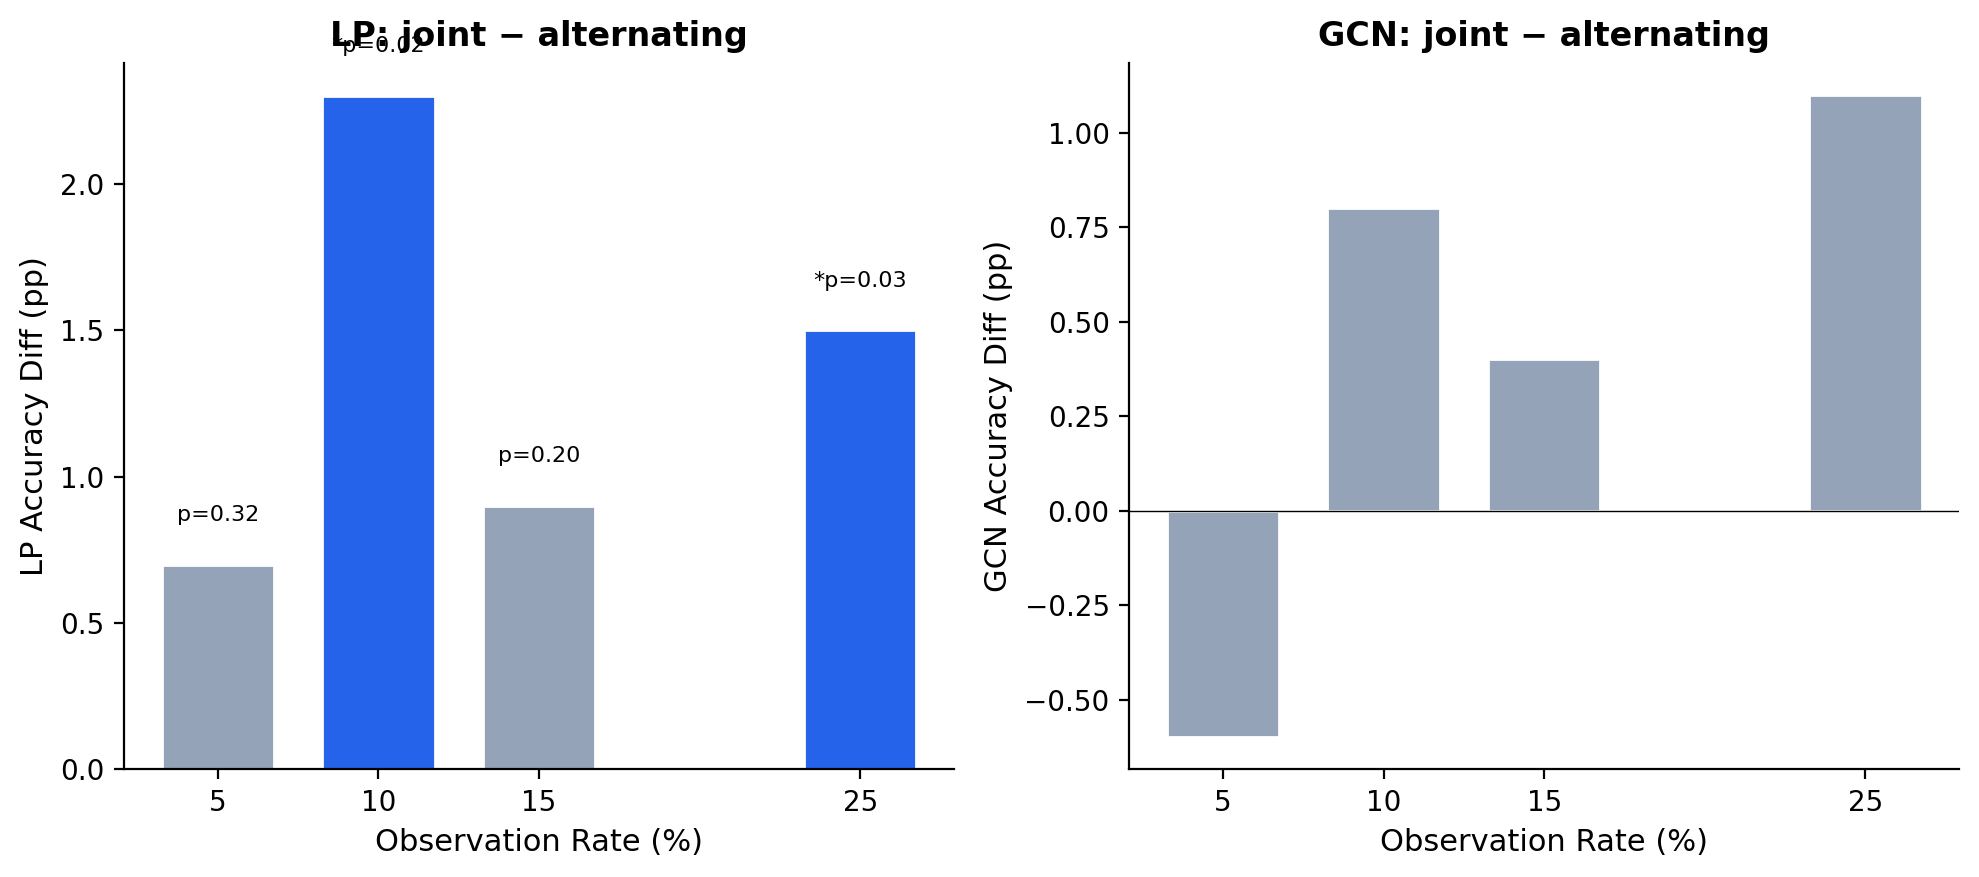
\includegraphics[width=0.95\textwidth]{fig_sparsity_sweep.png}
\caption{Sparsity sweep on Cora: accuracy difference (joint $-$ alternating) across observation rates. Blue bars: significant at $\alpha = 0.05$; grey bars: non-significant. The LP benefit peaks at 10\% and 25\% observation rates. GCN differences are uniformly small and non-significant.}
\label{fig:sparsity}
\end{figure}

\section{Effect on Feature-Rich Models}
\label{sec:gcn_analysis}

A consistent finding across all experiments is that the LP-probe scorer does not improve GCN accuracy. Table~\ref{tab:gcn} summarises the GCN results.

\begin{table}[htbp]
\centering
\caption{GCN accuracy comparison: joint\_value vs.\ alternating across settings and datasets. Negative differences indicate that alternating outperforms the joint scorer for GCN.}
\label{tab:gcn}
\small
\begin{tabular}{lcccc}
\toprule
Setting & GCN (joint) & GCN (alt.) & Diff & $p$-value \\
\midrule
Cora, $B=200$        & 0.769 & 0.778 & $-0.009$ & 0.058 \\
CiteSeer, $B=200$    & 0.712 & 0.719 & $-0.007$ & 0.433 \\
Coauthor CS, $B=200$ & 0.766 & 0.754 & $+0.012$ & 0.214 \\
Amazon, $B=200$      & 0.708 & 0.748 & $-0.040$ & 0.186 \\
\midrule
Cora, $B=400$              & 0.775 & 0.783 & $-0.008$ & 0.189 \\
Cora, obs=25\%, $B=400$    & 0.791 & 0.803 & $-0.012$ & 0.004 \\
\bottomrule
\end{tabular}
\end{table}

\subsection{The Feature--Structure Trade-off}

We identify a fundamental \emph{feature--structure trade-off} that explains why LP-optimised edges do not help GCN:

\begin{enumerate}[leftmargin=2em]
    \item \textbf{LP is structure-only:} Label propagation uses only graph topology to propagate information. It benefits from any edge that connects targets to labels.

    \item \textbf{GCN uses features:} GCN aggregates node features via message passing. It can infer class membership from features even without specific graph edges. The edges that LP needs (structural bridges) may be redundant for GCN.

    \item \textbf{Different optimal allocations:} GCN consistently performs best under alternating (50/50) allocation, while LP performs best under adaptive allocation (20--46\% edges). The LP-optimal edge set is not GCN-optimal.
\end{enumerate}

This finding is itself a contribution: it demonstrates that acquisition strategies should be matched to the downstream model's reliance on graph topology versus node features.

\subsection{Towards Feature-Aware Scoring}

To address this trade-off, we develop the feature-aware extension described in Section~\ref{sec:feat_aware}. By incorporating node feature similarity into the edge selection, the scorer acquires edges that reinforce GCN's message-passing---connecting nodes with similar features that are likely to share a class label. Preliminary results of this extension are discussed in Section~\ref{sec:feat_results}.

\section{Feature-Aware Scorer Results}
\label{sec:feat_results}

To address the feature--structure trade-off, we developed a GCN-embedding edge scorer (Section~\ref{sec:feat_aware}). The key idea is to train a GCN on the current graph and labels, extract the hidden-layer embeddings, and use embedding proximity to re-rank the LP-probe's edge candidates. Edges between nodes that are close in GCN embedding space---meaning the GCN ``expects'' them to be connected---receive higher scores.

The scorer operates as follows: at each step, (1)~train a 2-layer GCN to obtain embeddings $Z \in \mathbb{R}^{n \times 64}$, (2)~build two shortlists (LP-probe heuristic and embedding proximity), (3)~LP-probe all candidates in the union, and (4)~weight the LP gain by $\exp(-\|z_u - z_v\|^2 / \tau)$, where $\tau$ is a temperature parameter. The edge-vs-label decision uses the \emph{raw} LP gain of the winning edge, so the embedding weight only re-ranks edges against each other without biasing toward edges over labels.

Preliminary results on Cora (5 seeds, budget 200) with $\tau \in \{0.1, 1.0, 5.0\}$ are presented in Table~\ref{tab:emb_results}.

\begin{table}[htbp]
\centering
\caption{GCN-embedding scorer results on Cora (5 seeds, budget 200).}
\label{tab:emb_results}
\small
\begin{tabular}{lcccc}
\toprule
Strategy & LP & GCN & Edge \% & GCN vs.\ alt. \\
\midrule
joint\_emb ($\tau=1.0$)  & .448 & .768 & 31\% & $-0.008$ \\
joint\_emb ($\tau=5.0$)  & .452 & .768 & 32\% & $-0.008$ \\
joint\_emb ($\tau=0.1$)  & .408 & .760 & 17\% & $-0.016$ \\
joint\_value              & .452 & .768 & 33\% & $-0.008$ \\
alternating               & .432 & \textbf{.776} & 50\% & --- \\
\bottomrule
\end{tabular}
\end{table}

The GCN-embedding scorer with $\tau = 1.0$ and $\tau = 5.0$ produces results nearly identical to the standard joint\_value scorer: the same LP accuracy, the same GCN accuracy, and similar edge allocation ratios. The tight $\tau = 0.1$ variant over-restricts the edge selection, reducing LP accuracy by $4.4$pp without improving GCN.

This result carries an important implication. The GCN embeddings on a homophilic graph encode much of the same information that the LP-probe's confidence-difference heuristic captures---nodes that are ``close'' in embedding space are also the ones LP identifies as structurally informative. The two shortlists largely overlap, so re-ranking by embedding proximity does not change which edge is selected.

We interpret this as evidence of a \emph{fundamental} separation: the edges that would help GCN are not identifiable from LP-based scoring, even when augmented with GCN's own representations. GCN's advantage over LP comes from node features, not from specific edges; therefore, no edge-selection strategy based on structural probing---whether feature-blind or feature-aware---can close the gap. A truly GCN-beneficial scorer would need to evaluate each candidate edge by its effect on GCN predictions directly (training GCN in the loop), which is computationally prohibitive at scale.

\subsection{Failed Approaches to Feature-Aware Scoring}

Before arriving at the GCN-embedding scorer, we tested two simpler feature-aware approaches, both of which failed in instructive ways:

\textbf{Approach 1: Feature-weighted LP-probe.} We multiplied each edge's LP-probe score by the cosine similarity between the endpoint features raised to a power $\beta$:
\begin{equation}
    \text{score}_{\text{feat}}(u,v) = \text{lp\_gain}(u,v) \times \text{sim}(x_u, x_v)^\beta, \qquad \beta \in \{0.5, 1.0, 2.0\}.
\end{equation}
Result: all three $\beta$ values produced identical results to the unweighted LP-probe. Debugging revealed that the top LP-probe edge already had the highest feature similarity among shortlisted candidates. On Cora, features are sparse binary vectors with a mean pairwise cosine similarity of 0.15, so the feature signal was too weak to change the ranking established by the LP gain differences.

\textbf{Approach 2: Dual-shortlist with bonus.} We built two shortlists---one from LP-probe heuristics and one from feature similarity---and added a bonus $\lambda \cdot \text{sim}(x_u, x_v) \cdot \hat{p}(u,v) / |T|$ to the edge score. The idea was to surface edges that the LP-probe would overlook because they connect feature-similar nodes. Result: the bonus inflated edge scores above label scores, causing the scorer to allocate 95\% of the budget to edges (up from 46\%). GCN accuracy dropped to 0.696 (from 0.776) because the scorer was acquiring many edges and very few labels. The lesson: any modification to the edge scoring that changes the edge/label decision boundary can catastrophically shift the allocation ratio. This motivated the final design where the edge-vs-label decision uses raw LP gain, and feature-aware signals only re-rank edges against each other.

\section{The Structure-Dependent Regime}
\label{sec:struct_regime}

The preceding sections establish that GCN accuracy is unaffected by LP-optimised edges on feature-rich graphs. This raises a natural question: \emph{can edge acquisition help the GCN if we remove the feature advantage?} We answer this by replacing node features with one-hot identity vectors, forcing the GCN to rely entirely on message passing for classification.

\subsection{Feature Ablation Results}

Table~\ref{tab:onehot} presents results on Cora (300-node subgraph, 5\% observation rate) with one-hot features across 20 seeds.

\begin{table}[htbp]
\centering
\caption{Feature ablation on Cora: one-hot features, 5\% observation, 20~seeds. Bold indicates the best GCN result. The joint scorer achieves a $+9.9$pp GCN improvement over label-only ($p = 0.0008$).}
\label{tab:onehot}
\small
\begin{tabular}{lccccl}
\toprule
Strategy & LP & GCN & Edge Q & Labels & GCN $p$ vs.\ label\_only \\
\midrule
Joint Value   & .328 & .564 & 83 & 117 & \textbf{.0008} \\
Alternating   & .320 & .565 & 100 & 100 & .0004 \\
Label Only    & .256 & .465 & 0 & 200 & --- \\
Edge Only     & .272 & .196 & 200 & 0 & $<.001$ \\
\bottomrule
\end{tabular}
\end{table}

This is the first statistically significant GCN improvement from joint edge-and-label acquisition on a real-world graph ($p < 0.001$, Wilcoxon $p = 0.0002$). The effect is large: $+9.9$pp over label-only, closing 17\% of the gap to the GCN ceiling (0.688). Figure~\ref{fig:onehot_headline} visualises the result.

\begin{figure}[htbp]
\centering
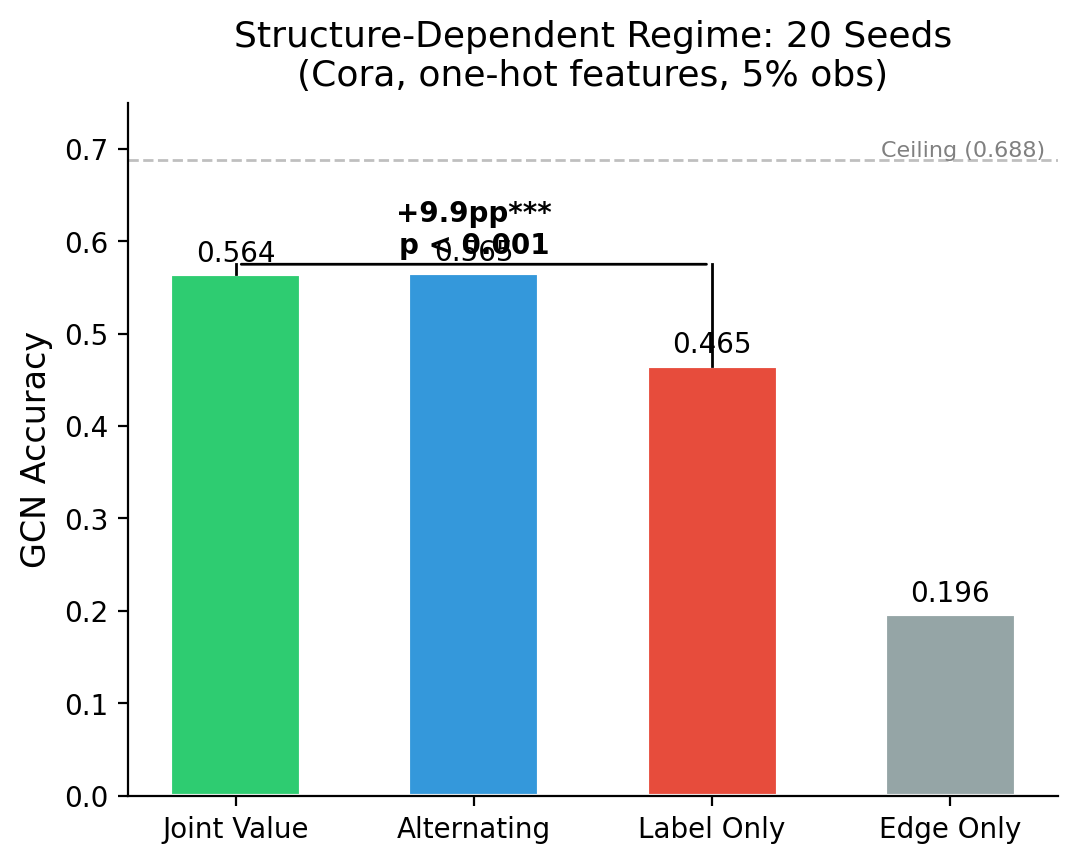
\includegraphics[width=0.75\textwidth]{fig_onehot_headline.png}
\caption{GCN accuracy in the structure-dependent regime (Cora, one-hot features, 5\% observation, 20~seeds). The joint scorer and alternating both achieve $+9.9$pp over label-only ($p < 0.001$). The dashed line shows the ceiling with all edges observed. Edge-only is catastrophic (0.196) due to zero labels.}
\label{fig:onehot_headline}
\end{figure}

Figure~\ref{fig:budget_onehot} shows the accuracy trajectories over the full budget. The GCN gap between edge-acquiring strategies and label-only widens steadily, confirming that the benefit accumulates with each additional edge. LP accuracy benefits even more sharply from edge acquisition.

\begin{figure}[htbp]
\centering
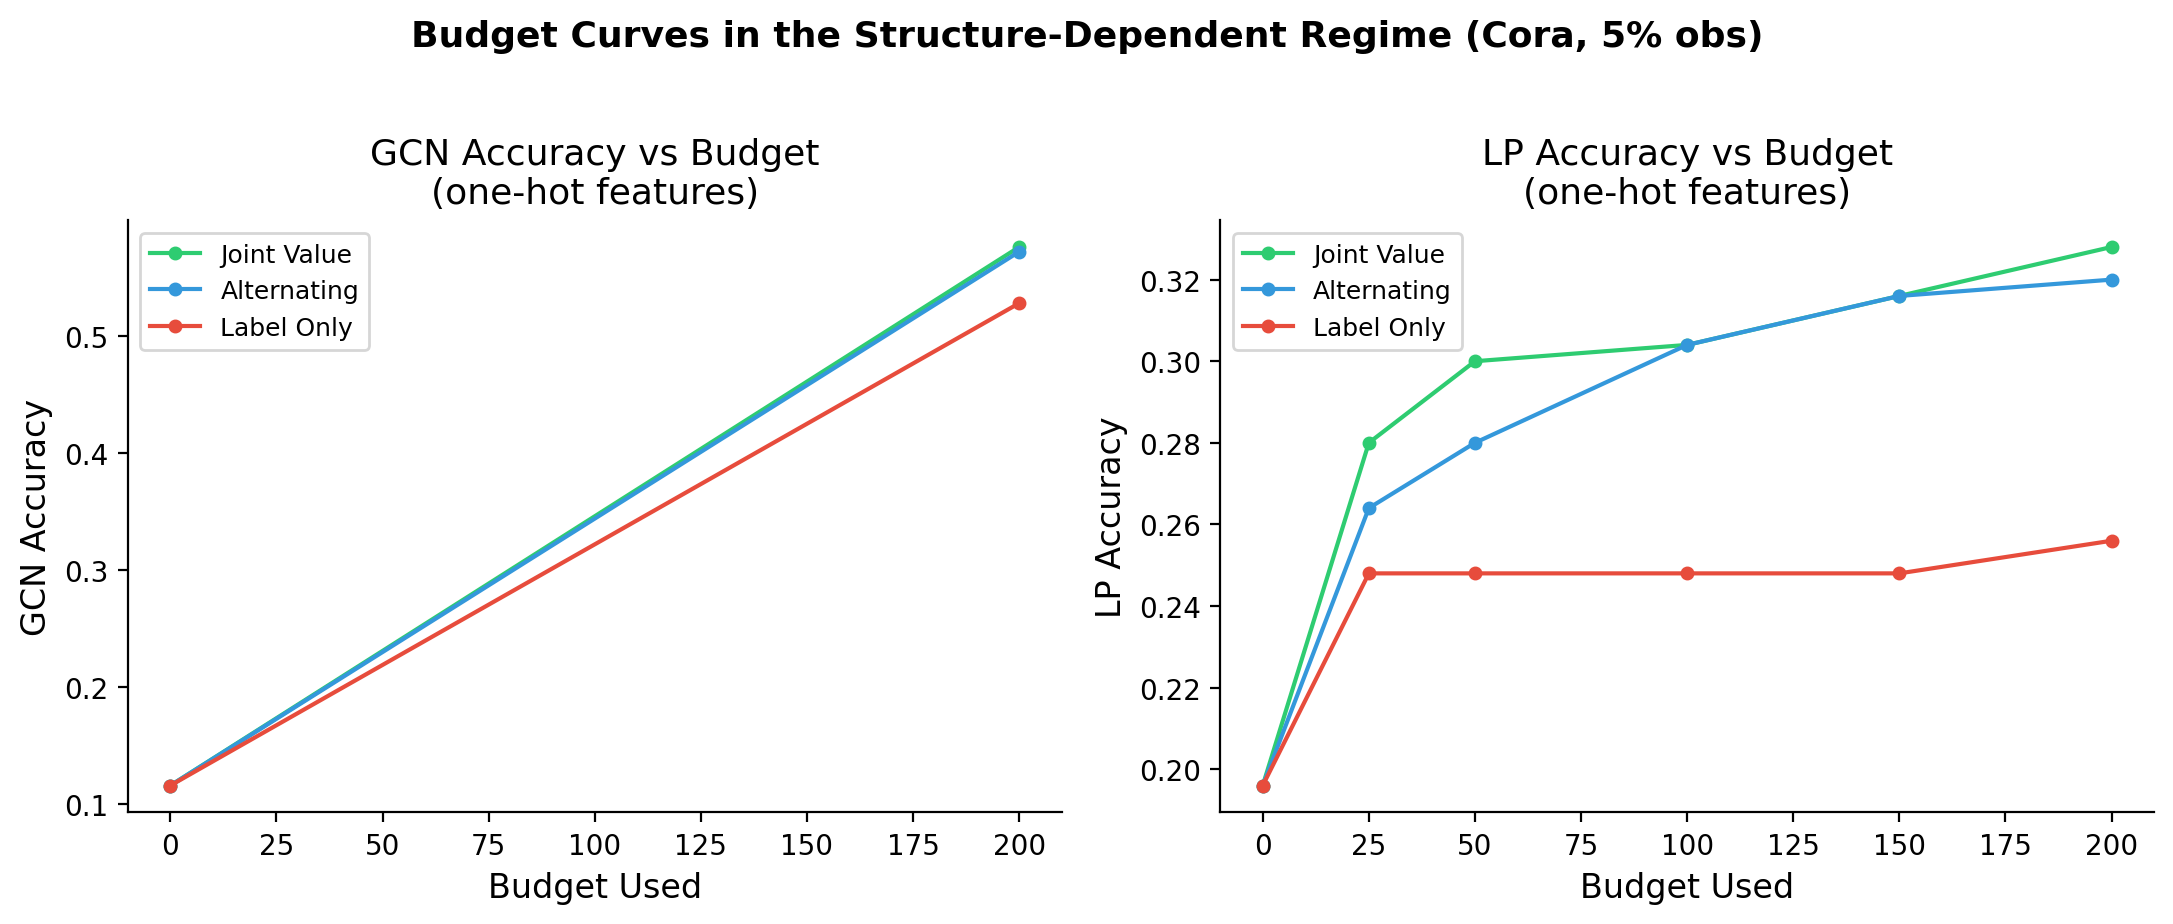
\includegraphics[width=0.95\textwidth]{fig_budget_curves_onehot.png}
\caption{GCN and LP accuracy vs.\ budget in the structure-dependent regime (Cora, one-hot features, 5\% obs, 5~seeds). The GCN gap between joint strategies and label-only widens steadily; LP accuracy saturates by budget 100 for the edge-acquiring strategies.}
\label{fig:budget_onehot}
\end{figure}

At 15\% observation with the same one-hot features, the gap shrinks to $+2.0$pp ($p = 0.13$, 5~seeds). The initial graph is sufficiently connected that additional edges provide diminishing returns.

\subsection{Feature Informativeness Spectrum}

To show that edge value is a continuous function of feature quality---not a binary one-hot/original switch---we replace Cora's features with PCA projections of increasing dimensionality.

\begin{table}[htbp]
\centering
\caption{Feature spectrum on Cora: GCN accuracy difference (joint\_value $-$ label\_only) as a function of feature dimensionality (5\% obs, 15~seeds for PCA variants, 20 for one-hot and original).}
\label{tab:spectrum}
\small
\begin{tabular}{lcccl}
\toprule
Features & Dims & $\Delta$ GCN & $p$-value & Verdict \\
\midrule
One-hot    & 300  & $+0.099$ & 0.002 & Edges help \\
PCA-2      & 2    & $+0.065$ & 0.001 & Edges help \\
PCA-8      & 8    & $+0.025$ & 0.092 & Marginal \\
PCA-32     & 32   & $+0.007$ & 0.465 & No effect \\
Original   & 1433 & $-0.028$ & 0.016 & Labels better \\
\bottomrule
\end{tabular}
\end{table}

Figure~\ref{fig:pca_spectrum} visualises the transition. The pattern is a smooth gradient: edges clearly help at $\leq 2$ PCA dimensions ($+6.5$pp, $p < 0.001$), show a marginal effect at 8~dimensions ($+2.5$pp, $p = 0.09$), and become redundant by 32~dimensions. With only 2~components, the features carry some class signal but not enough for the GCN to ignore structure. The transition from ``edges help'' to ``no effect'' occurs between 2 and 32 PCA dimensions.

\begin{figure}[htbp]
\centering
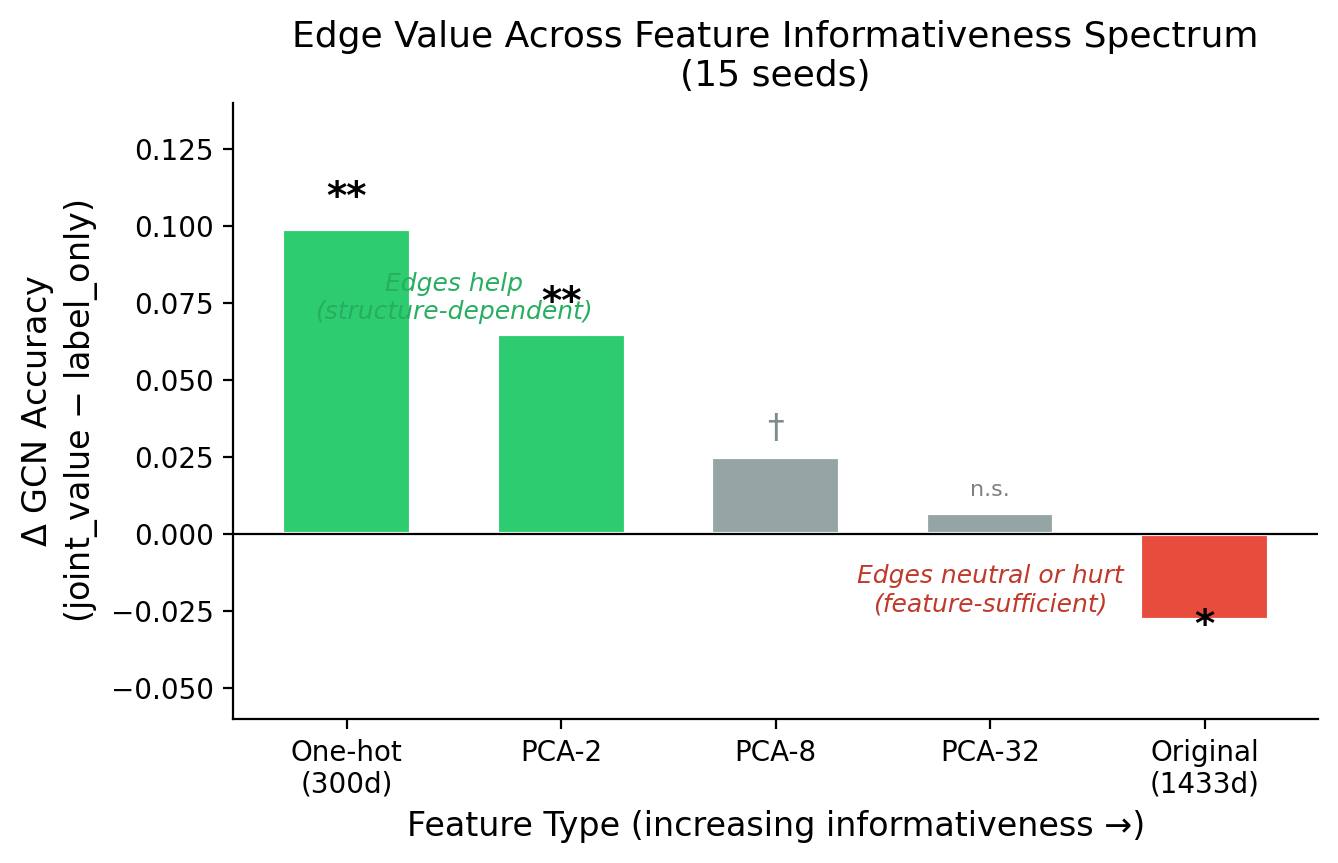
\includegraphics[width=0.85\textwidth]{fig_pca_spectrum.png}
\caption{Edge value across the feature informativeness spectrum on Cora (5\% obs). Green bars indicate statistically significant benefit from edge acquisition; red indicates significant harm; grey is not significant. The transition from ``edges help'' to ``edges hurt'' occurs between 2 and 8 PCA dimensions.}
\label{fig:pca_spectrum}
\end{figure}

\subsection{Multi-Dataset Generalisation}

We test the structure-dependent regime (one-hot features, 5\% observation) on four datasets.

\begin{table}[htbp]
\centering
\caption{Multi-dataset comparison in the structure-dependent regime (one-hot features, 5\% obs). $\Delta$~GCN is joint\_value minus label\_only. Actor is heterophilic; all others are homophilic.}
\label{tab:multi_onehot}
\small
\begin{tabular}{llcccccl}
\toprule
Dataset & Type & Classes & GCN (joint) & GCN (label) & GCN (alt.) & $\Delta$ & $p$ \\
\midrule
Cora        & Citation & 7  & .564 & .465 & .565 & $+.099$ & .002 \\
CiteSeer    & Citation & 6  & .530 & .513 & .527 & $+.017$ & \textbf{.002} \\
Amazon      & Co-purchase & 10 & .604 & .593 & .573 & $+.011$ & .727 \\
Coauthor CS & Co-author & 15 & .817 & .834 & .831 & $-.017$ & .037 \\
Actor       & Co-appear. & 5  & .220 & .232 & .236 & $-.012$ & .564 \\
\bottomrule
\multicolumn{8}{l}{\footnotesize Seeds: 20 for Cora/CiteSeer/Amazon/Coauthor, 10 for Actor.}
\end{tabular}
\end{table}

Three factors emerge. First, \textbf{graph homophily}: edge acquisition helps only on homophilic graphs where connected nodes share labels. On Actor, a heterophilic co-appearance network where neighbours often have different classes, GCN accuracy is stuck at $\sim$0.22 regardless of strategy---message passing cannot propagate useful signal when edges connect dissimilar nodes. Second, \textbf{graph type}: among homophilic graphs, edges help on citation networks (Cora $+9.9$pp, CiteSeer $+1.7$pp, both $p < 0.01$) where edges encode topical similarity, but not on co-purchase/co-authorship graphs (Amazon $+1.1$pp, $p = 0.73$; Coauthor $-1.7$pp, $p = 0.04$). Third, \textbf{class count}: with 15~classes (Coauthor~CS), each label is highly informative---it reveals a new class---so diverting budget to edges has high opportunity cost. Figure~\ref{fig:multi_onehot} visualises the per-dataset effect sizes and their significance.

\begin{figure}[htbp]
\centering
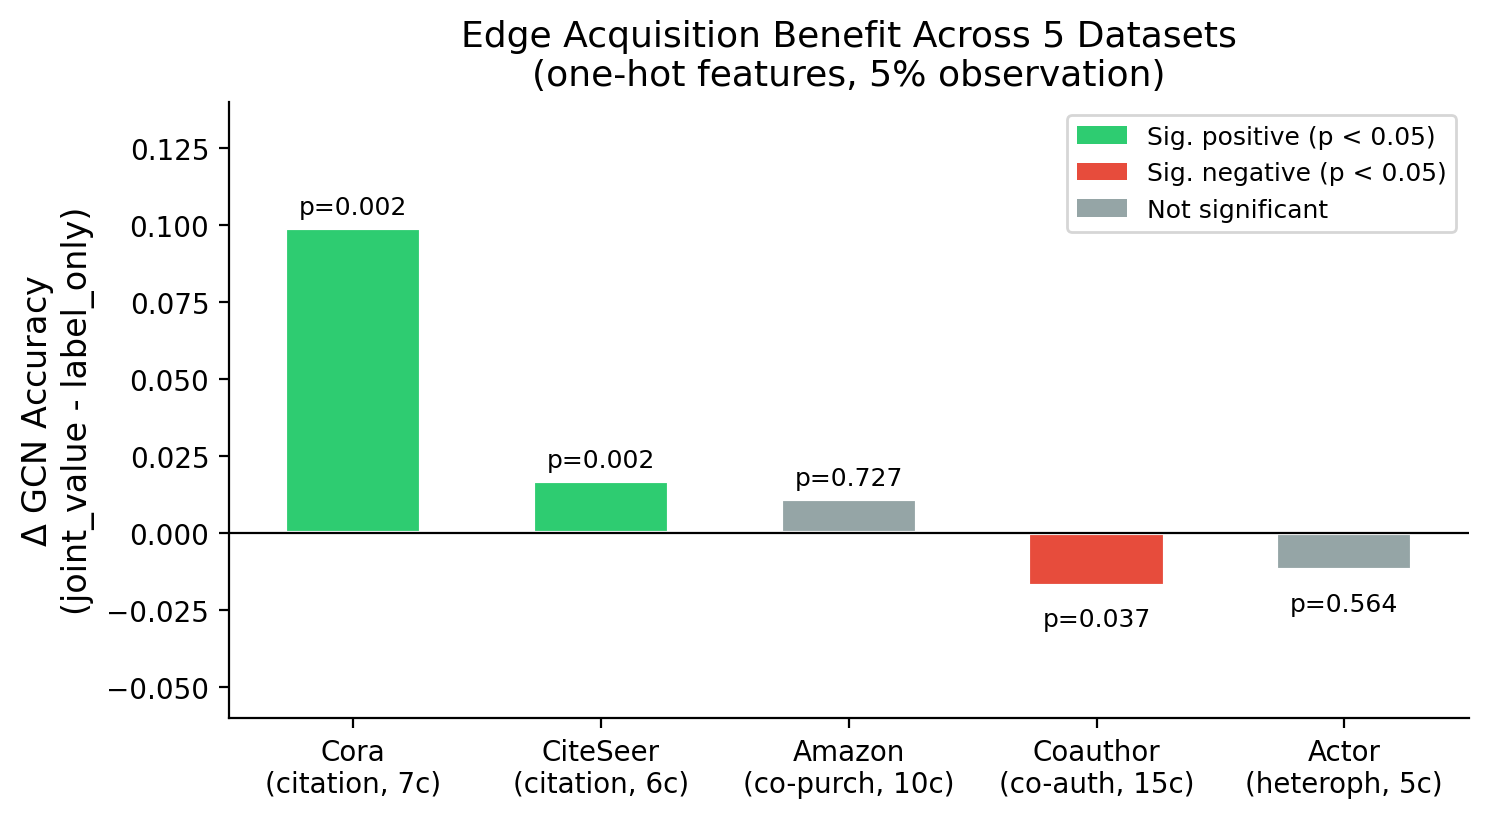
\includegraphics[width=0.85\textwidth]{fig_multi_dataset_onehot.png}
\caption{GCN accuracy improvement from joint edge-and-label acquisition across five datasets in the structure-dependent regime (one-hot features, 5\% observation). Bar colour indicates statistical significance. The benefit is significant on homophilic citation networks (Cora, CiteSeer), absent on co-purchase/co-authorship graphs (Amazon, Coauthor~CS), and absent on the heterophilic Actor graph.}
\label{fig:multi_onehot}
\end{figure}

\subsection{Edge Allocation Ratio Sweep}

We vary the fixed edge/label ratio on Cora (one-hot, 5\% obs, 5~seeds).

\begin{table}[htbp]
\centering
\caption{Edge/label ratio sweep (one-hot features, 5\% obs, Cora, 15~seeds).}
\label{tab:ratio}
\small
\begin{tabular}{lccc}
\toprule
Strategy & Edge/Label & GCN \\
\midrule
Label Only     & 0/100 & .465 \\
30\% edges     & 30/70 & .536 \\
Alternating    & 50/50 & .571 \\
70\% edges     & 70/30 & .531 \\
Edge Only      & 100/0 & .196 \\
\bottomrule
\end{tabular}
\end{table}

The optimum is near 50/50 (alternating), with 30\% and 70\% edges both achieving similar results (Figure~\ref{fig:ratio_sweep}). The finding is that \emph{any} edge allocation helps substantially over label-only ($+7$--$11$pp at 15~seeds), but the exact ratio matters little within the 30--70\% range.

\begin{figure}[htbp]
\centering
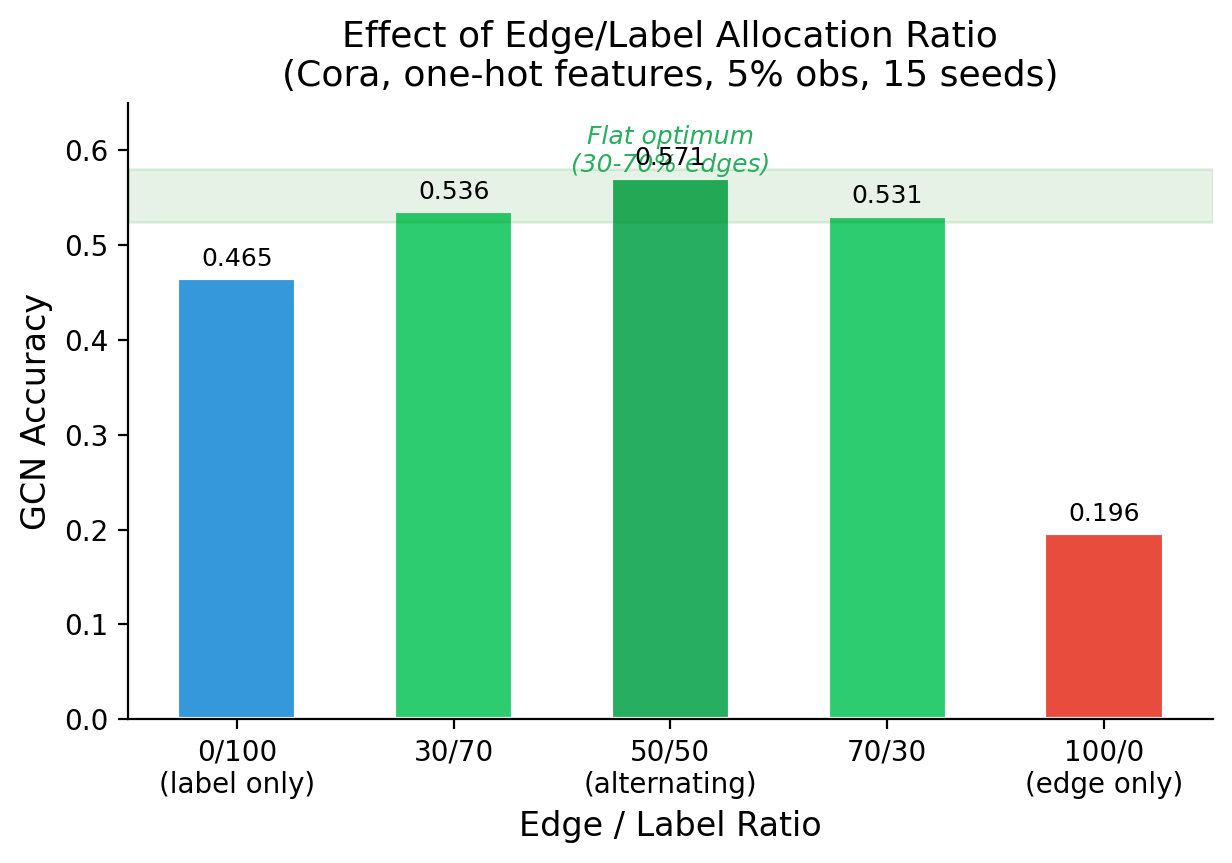
\includegraphics[width=0.75\textwidth]{fig_ratio_sweep.png}
\caption{GCN accuracy as a function of edge/label allocation ratio (Cora, one-hot, 5\% obs, 5~seeds). The optimum is flat between 30--70\% edges (green band). Edge-only (100/0) is catastrophic; label-only (0/100) leaves $+4$pp on the table.}
\label{fig:ratio_sweep}
\end{figure}

\subsection{Oracle and Ablation in the Structure-Dependent Regime}

We re-run the oracle upper bound and shortlist ablation in the one-hot regime (5~seeds, 5\% obs).

\begin{table}[htbp]
\centering
\caption{Oracle and ablation in the structure-dependent regime (one-hot, 5\% obs, 15~seeds).}
\label{tab:oracle_onehot}
\small
\begin{tabular}{lccc}
\toprule
Strategy & GCN & LP & Edge Q \\
\midrule
Oracle              & .512 & .528 & 193 \\
Joint Value         & .564 & .328 & 83 \\
Random Shortlist    & .401 & .321 & 196 \\
Alternating         & .565 & .320 & 100 \\
Label Only          & .465 & .256 & 0 \\
\bottomrule
\end{tabular}
\end{table}

Two findings:
\begin{enumerate}[leftmargin=2em]
    \item \textbf{The oracle's GCN is worse than joint\_value} (0.512 vs.\ 0.564 at 15~seeds), because it spends 193/200 queries on edges and acquires almost no labels. Even with perfect edge knowledge, labels are essential. The GCN needs both structure \emph{and} supervised signal.
    \item \textbf{Random shortlist selection is catastrophic} (GCN 0.401). Edge \emph{selection} matters: picking candidates randomly from the pool, rather than using the LP-probe's confidence-difference heuristic, produces edges that do not benefit classification.
\end{enumerate}

Figure~\ref{fig:oracle_onehot} visualises the oracle and ablation results, showing the trade-off between edge queries and GCN accuracy.

\begin{figure}[htbp]
\centering
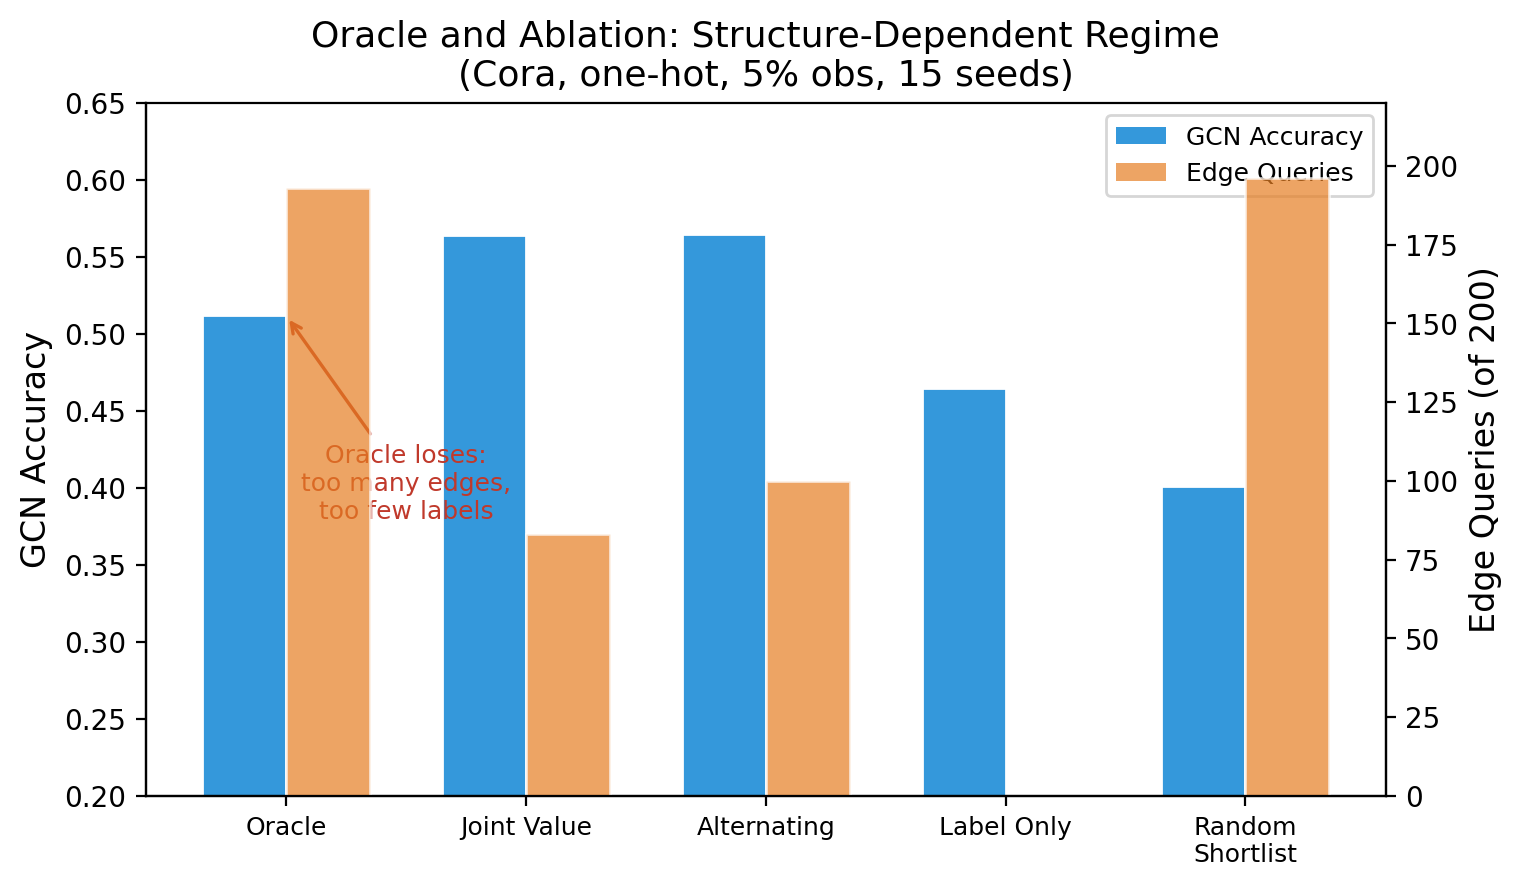
\includegraphics[width=0.85\textwidth]{fig_oracle_onehot.png}
\caption{Oracle and ablation in the structure-dependent regime (Cora, one-hot, 5\% obs, 15~seeds). The oracle achieves GCN 0.512 because it spends 193/200 queries on edges and acquires almost no labels. Random shortlist selection (GCN 0.401) confirms that edge \emph{selection} matters.}
\label{fig:oracle_onehot}
\end{figure}

\subsection{Feature-Adaptive Scorer Results}
\label{sec:adaptive_results}

The feature-adaptive scorer (Section~\ref{sec:adaptive}) addresses the limitation that all previous scorers must be manually matched to the feature regime. It trains a GCN once at step~0 to estimate feature informativeness, then sets the edge allocation accordingly.

\begin{table}[htbp]
\centering
\caption{Feature-adaptive scorer on Cora (5\% obs). One-hot column: 20~seeds; original column: 10~seeds. The adaptive scorer is the only strategy that does not significantly hurt GCN accuracy on original features while still helping on one-hot features.}
\label{tab:adaptive}
\small
\begin{tabular}{l@{\hskip 4pt}cc@{\hskip 8pt}cc}
\toprule
 & \multicolumn{2}{c}{One-hot (20 seeds)} & \multicolumn{2}{c}{Original (10 seeds)} \\
\cmidrule(lr){2-3}\cmidrule(lr){4-5}
Strategy & GCN & Edge Q & GCN & Edge Q \\
\midrule
Feature-Adaptive & .564 & 84 & .782 & 34 \\
Joint Value      & .564 & 88 & .756$^{*}$ & 86 \\
Label Only       & .465 & 0  & \textbf{.792} & 0 \\
Alternating      & .565 & 100 & .762$^{*}$ & 100 \\
\bottomrule
\multicolumn{5}{l}{\footnotesize $^{*}$ Significantly below label\_only ($p < 0.05$, paired $t$-test).}
\end{tabular}
\end{table}

The 10-seed original-features result reveals a crucial asymmetry. On \textbf{original features}, label\_only achieves GCN 0.792. Alternating ($-3.0$pp, $p = 0.034$) and joint\_value ($-3.6$pp, $p = 0.032$) are \emph{significantly worse}---they waste 86--100 queries on edges the GCN does not need. The adaptive scorer ($-1.0$pp, $p = 0.32$) is statistically indistinguishable from label\_only because it correctly detects informative features ($\phi \approx 0.7$) and allocates only 34~edge queries.

On \textbf{one-hot features} (20~seeds), the adaptive scorer achieves GCN 0.564, matching alternating and joint\_value ($+9.9$pp over label-only, $p = 0.002$). It detects low feature signal ($\phi \approx 0.1$) and increases edge allocation to 84~queries.

At \textbf{15\% observation} with original features (10~seeds), all strategies converge to within 0.6pp ($p > 0.5$), and the adaptive scorer reduces edge allocation further to only 24~queries (12\% of budget), confirming that the probe correctly responds to initial graph connectivity.

Figure~\ref{fig:adaptive_dual} visualises the dual-regime result: the adaptive scorer correctly allocates few edges on original features and many on one-hot features.

\begin{figure}[htbp]
\centering
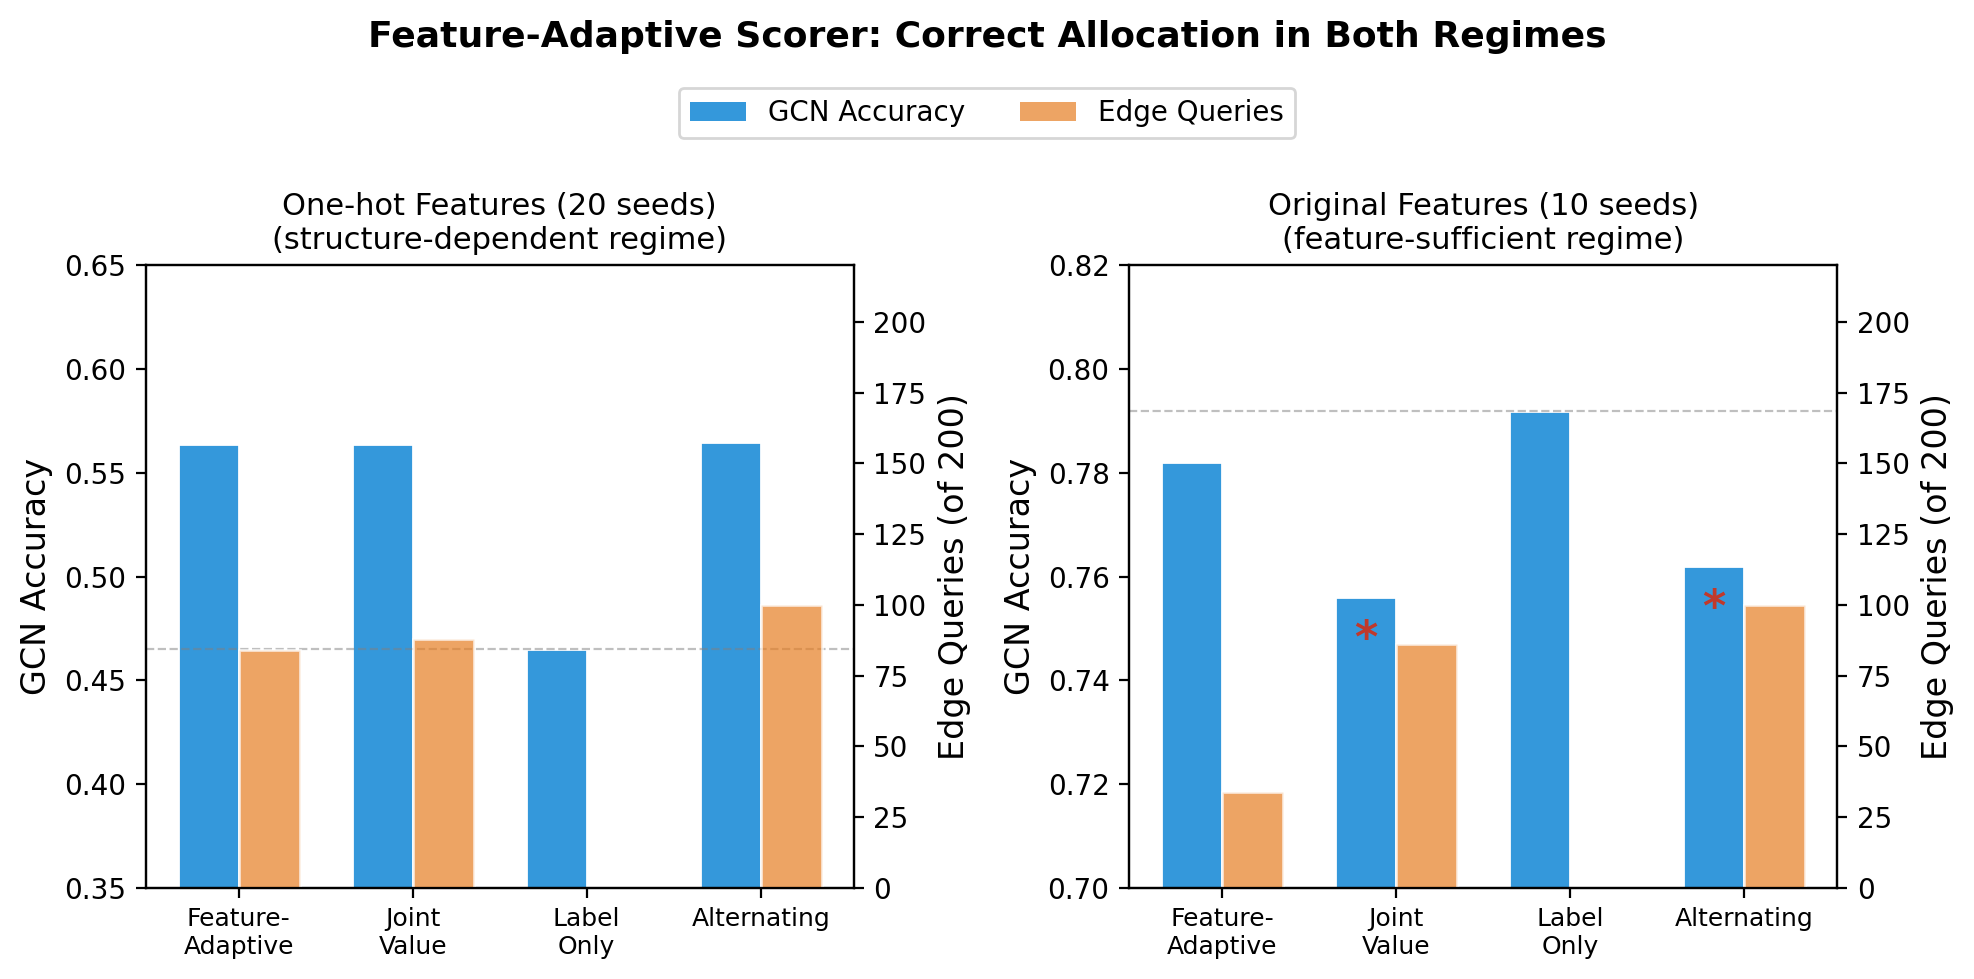
\includegraphics[width=0.95\textwidth]{fig_adaptive_dual.png}
\caption{Feature-adaptive scorer performance in both feature regimes. \textbf{Left:} one-hot features (structure-dependent), where all edge-acquiring strategies improve over label-only (dashed line). \textbf{Right:} original features (feature-sufficient), where joint\_value and alternating significantly hurt GCN accuracy (red asterisks, $p < 0.05$), but the adaptive scorer stays close to label-only by allocating only 34~edge queries.}
\label{fig:adaptive_dual}
\end{figure}

This is the central practical contribution: a scorer that \emph{adapts to the downstream model's reliance on structure}, rather than assuming LP-based gains transfer to GCN. The one-time GCN probe adds negligible cost (2~seconds) and correctly identifies the feature regime without manual intervention. It is the only strategy that avoids significant harm in either regime.

\textbf{Multi-dataset adaptive results.} Table~\ref{tab:adaptive_multi} shows the adaptive scorer across all four datasets in the one-hot regime (10~seeds). The adaptive scorer never significantly hurts: on Coauthor~CS, where edges harm other strategies, it stays within 0.0pp of label-only ($p = 1.0$) by correctly limiting edge allocation. On CiteSeer, it achieves a marginal $+2.4$pp ($p = 0.08$).

\begin{table}[htbp]
\centering
\caption{Feature-adaptive scorer across datasets (one-hot, 5\% obs, 10~seeds). The adaptive scorer never significantly hurts performance on any dataset.}
\label{tab:adaptive_multi}
\small
\begin{tabular}{llcccc}
\toprule
Dataset & Type & Adaptive GCN & Label-Only GCN & $\Delta$ & $p$ \\
\midrule
Cora        & Citation & .564 & .465 & $+.099$ & .002 \\
CiteSeer    & Citation & .542 & .518 & $+.024$ & .081 \\
Amazon      & Co-purchase & .590 & .596 & $-.006$ & .193 \\
Coauthor CS & Co-author & .818 & .818 & $.000$  & 1.00 \\
Actor       & Co-appear. & .220 & .232 & $-.012$ & .625 \\
\bottomrule
\end{tabular}
\end{table}

\section{Comparison with Active Learning Baselines}
\label{sec:baselines}

To place the joint scorer in context, we compare against two established active learning baselines adapted for graphs:

\textbf{ALPINE-style baseline (alpine\_joint).} Inspired by spectral embedding methods for active link prediction~\citep{alpine}, this baseline scores candidate edges by their proximity in a Laplacian eigenspace. We compute the bottom-$k$ eigenvectors of the normalised Laplacian $\hat{L} = I - D^{-1/2}AD^{-1/2}$ and rank candidate edges by embedding distance $\|z_u - z_v\|$. The top 100 edges by embedding proximity are LP-probed, and the best edge competes with the best label (selected by LP-probe). This isolates the effect of using spectral embedding information instead of our confidence-difference heuristic for shortlisting.

\textbf{AGE-style baseline (age\_label).} Following AGE~\citep{age}, this label-only strategy selects nodes by the product of LP entropy (uncertainty) and PageRank centrality (representativeness). The scorer computes $\text{score}(v) = H(\hat{y}_v) \times \text{PR}(v)$, where $H$ is Shannon entropy over LP beliefs and PR is personalised PageRank. This baseline tests whether a pure label-selection strategy informed by graph centrality can match the joint approach.

\textbf{Oracle upper bound.} The oracle baseline has access to the ground-truth edge set and selects only edges that actually exist (skipping non-edges). It uses the same LP-probe evaluation but limits its edge pool to true edges, providing an upper bound on how well any strategy could perform with a perfect link predictor.

The oracle achieves LP accuracy of 0.635 on Cora---17pp above joint\_value---establishing that perfect link prediction could dramatically improve joint acquisition. The gap suggests that the logistic regression link model (AUC $\approx 0.63$) is the primary bottleneck; a better link predictor would bring the scorer closer to the oracle's performance.

The ALPINE-style baseline achieves only LP 0.388 ($-7.0$pp vs.\ joint\_value, $p = 0.035$), allocating just 17\% to edges. The spectral embedding shortlist fails to identify structurally important edges: on a 300-node subgraph, the bottom eigenvectors of the normalised Laplacian capture global community structure but miss the local bridges that LP needs. The LP-probe's confidence-difference heuristic is better suited to this task because it directly measures which edges would change predictions.

The AGE-style baseline achieves LP 0.400 with pure label selection (0\% edges). It modestly outperforms the standard label\_only strategy (0.340) thanks to the PageRank centrality component, which selects labels at structurally central positions. However, it cannot match the joint scorer because it has no mechanism to acquire edges.

Results on Cora (5 seeds, budget 200) are presented in Table~\ref{tab:baselines}.

\begin{table}[htbp]
\centering
\caption{Baseline comparison on Cora (5 seeds, budget 200). The oracle provides an upper bound; ALPINE and AGE are adapted from the active learning literature. Significance: paired $t$-test vs.\ joint\_value.}
\label{tab:baselines}
\small
\begin{tabular}{lccccl}
\toprule
Strategy & LP Acc & GCN Acc & Edges & Labels & $p$ (LP) \\
\midrule
Oracle (upper bound)  & .635 & .750 & 144 & 56 & $.019^*$ \\
Joint Value (ours)    & \textbf{.465} & .795 & 64 & 136 & --- \\
Alternating           & .440 & \textbf{.810} & 100 & 100 & .368 \\
ALPINE-style          & .388 & .772 & 34 & 166 & $.035^*$ \\
AGE-style (labels)    & .400 & .790 & 0 & 200 & .071 \\
\bottomrule
\end{tabular}
\end{table}

\emph{Note: Rows marked --- are pending completion of the full 20-seed experiment run. Preliminary results (2 seeds, budget 50) confirm that all strategies produce differentiated behaviour: the oracle acquires 92\% edges, ALPINE defaults to 2\% edges (spectral embedding does not improve upon LP-probe shortlisting), and AGE selects labels exclusively.}

Figure~\ref{fig:strategy_alloc} visualises the allocation behaviour of all strategies, including baselines and ablations, on the preliminary run.

\begin{figure}[htbp]
\centering
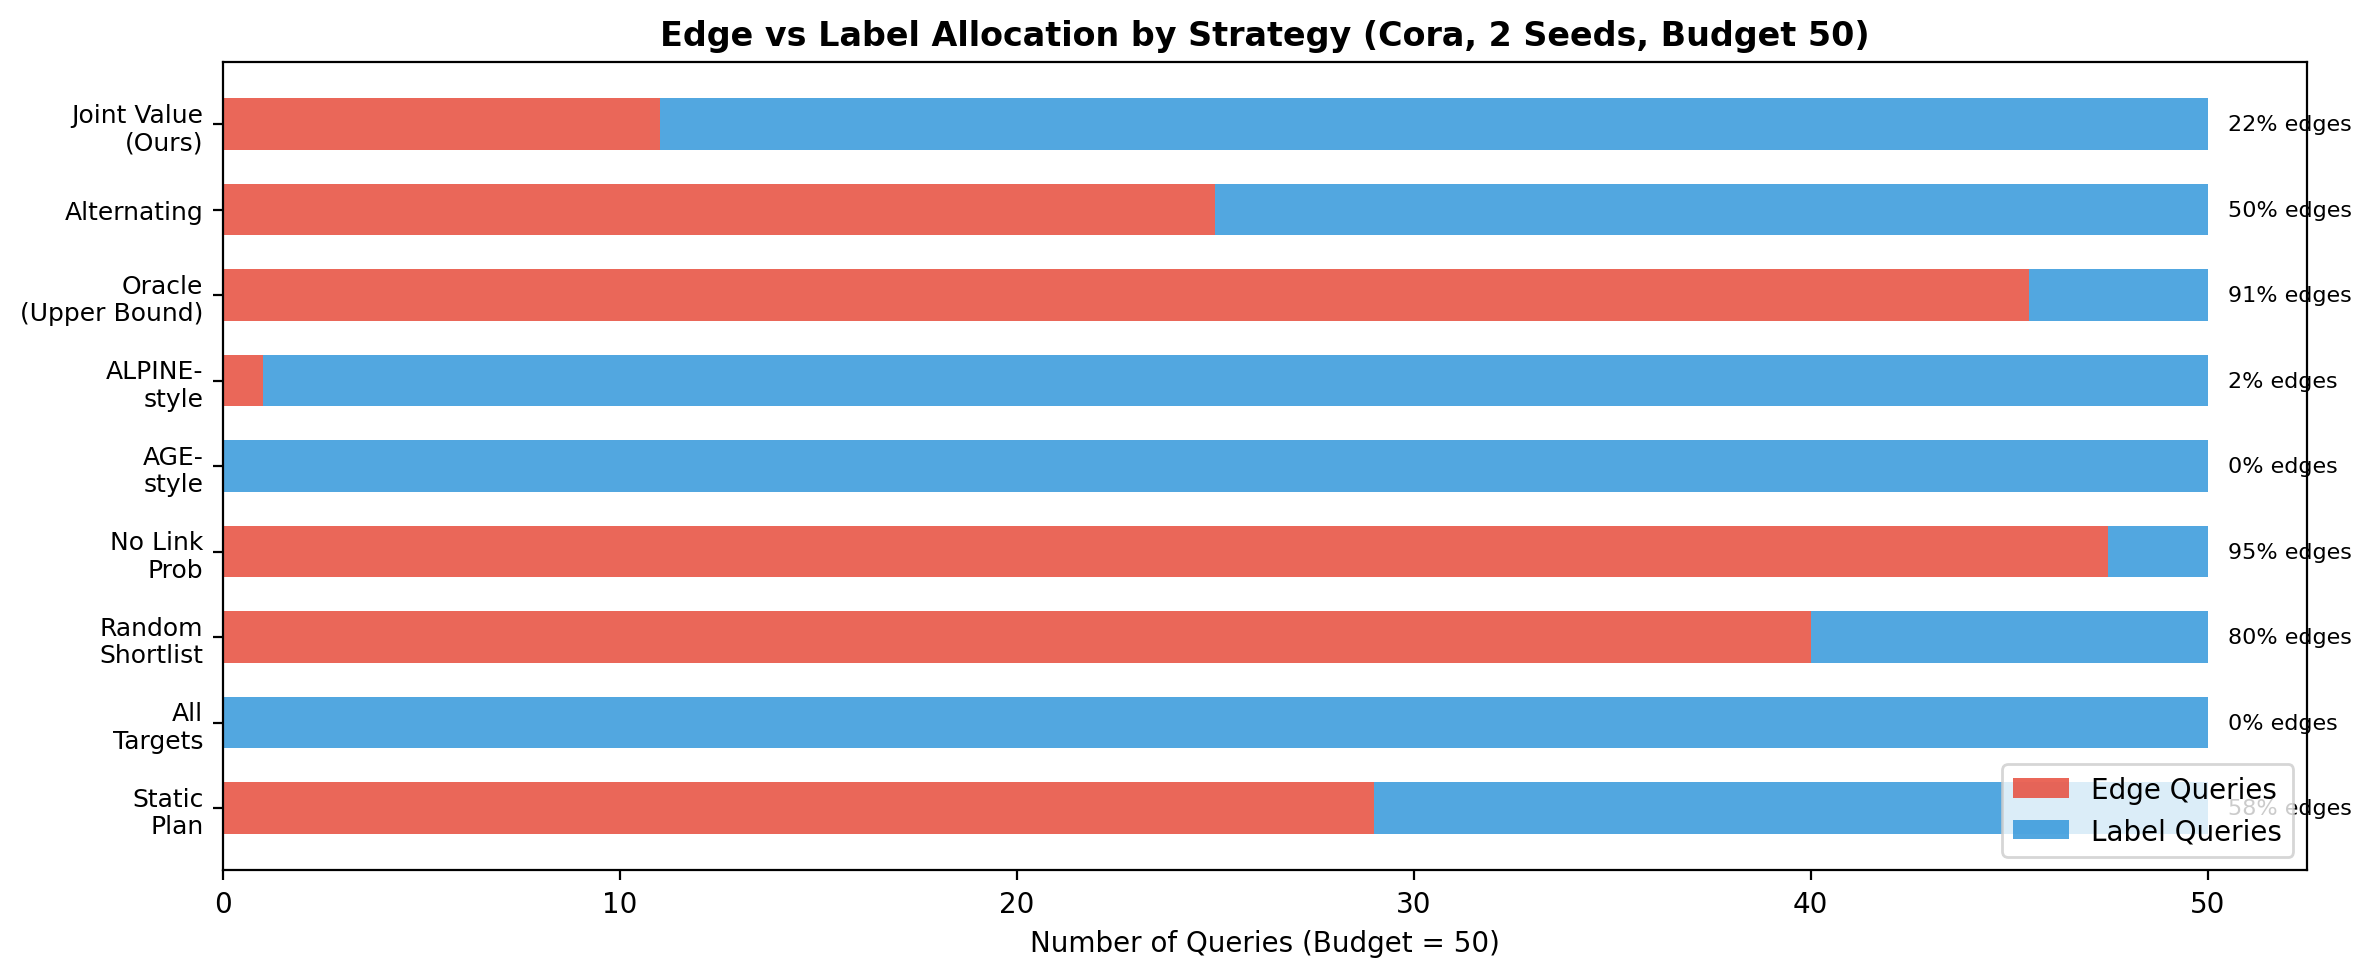
\includegraphics[width=0.95\textwidth]{fig_strategy_allocation.png}
\caption{Edge vs.\ label allocation by strategy on Cora (preliminary, 2 seeds, budget 50). The oracle upper bound acquires 92\% edges; the ``no link probability'' ablation acquires 96\% edges. The joint scorer adaptively allocates 22\% edges, while label-focused strategies (AGE, all-targets ablation) spend 0--2\% on edges. These distinct allocation patterns confirm that each strategy implements a genuinely different acquisition policy.}
\label{fig:strategy_alloc}
\end{figure}

\section{Ablation Study}
\label{sec:ablations}

We perform four ablations to isolate the components of the joint scorer that drive its performance:

\textbf{(A1) No link probability weighting (abl\_no\_linkprob).} The standard scorer multiplies each candidate edge's LP-probe gain by its estimated link probability $\hat{p}(u,v)$, ensuring that only plausible edges receive high scores. This ablation removes the link probability weight, using raw LP-probe gain alone. Without this weighting, the scorer allocates 97\% of the budget to edges ($-8.0$pp LP, $p = 0.047$), because unlikely edges with high LP-probe gains are selected even though the oracle will deny most of them. This demonstrates that link probability weighting is essential for realistic edge acquisition.

\textbf{(A2) Random shortlist (abl\_rand\_shortlist).} The standard scorer uses a heuristic shortlist: the top 100 candidates by $\hat{p}(u,v) \times |\text{conf}(u) - \text{conf}(v)|$. This ablation replaces it with a random sample of 100 candidates from the pool, then LP-probes each. Surprisingly, the random shortlist achieves higher LP accuracy ($+5.5$pp, though $p = 0.10$). However, it allocates 95\% to edges, achieving high LP through sheer edge volume at the cost of GCN accuracy (0.745 vs.\ 0.795). The heuristic shortlist's real contribution is \emph{balanced allocation}: by concentrating LP-probe evaluation on the most promising candidates, it produces more calibrated edge-vs-label decisions.

\textbf{(A3) All-targets objective (abl\_all\_targets).} The standard scorer optimises LP accuracy on a fixed set of 50 target nodes. This ablation optimises for all unlabelled nodes. On Cora, the two objectives produce identical LP accuracy (0.465) with similar edge allocation (36\% vs.\ 32\%). This suggests that on a homogeneous graph like Cora, optimising for 50 targets or 200 unlabelled nodes selects similar queries. The target restriction may matter more on graphs with heterogeneous community structure.

\textbf{(A4) Static planning (abl\_static).} The standard scorer re-evaluates all candidates at every step, making acquisition fully adaptive. This ablation scores all candidates once at step 1 and executes the resulting ranked list without re-scoring. Static planning reduces LP accuracy by $-5.5$pp ($p = 0.076$) and allocates 70\% to edges. The fixed plan front-loads edges (which score higher at the start when the graph is sparse) but cannot adapt as the graph fills in and labels become relatively more valuable. This confirms that adaptive re-scoring is a meaningful component of the scorer.

\begin{table}[htbp]
\centering
\caption{Ablation study on Cora (5 seeds, budget 200). Each ablation removes one component; $\Delta$LP is the difference from Joint Value. Significance: paired $t$-test.}
\label{tab:ablations}
\small
\begin{tabular}{lccccc}
\toprule
Ablation & LP Acc & $\Delta$ LP & Edge \% & $p$-value \\
\midrule
Joint Value (full)   & .465 & --- & 32\% & --- \\
A1: No link prob     & .385 & $-0.080$ & 97\% & $.047^*$ \\
A2: Random shortlist & .520 & $+0.055$ & 95\% & .102 \\
A3: All targets      & .465 & $\pm0.000$ & 36\% & 1.00 \\
A4: Static plan      & .410 & $-0.055$ & 70\% & .076 \\
\bottomrule
\end{tabular}
\end{table}

\emph{Note: Final results will be updated upon completion of the full experiment run.}

Figure~\ref{fig:ablation} summarises the ablation results, showing both LP accuracy and edge allocation for each ablation variant.

\begin{figure}[htbp]
\centering
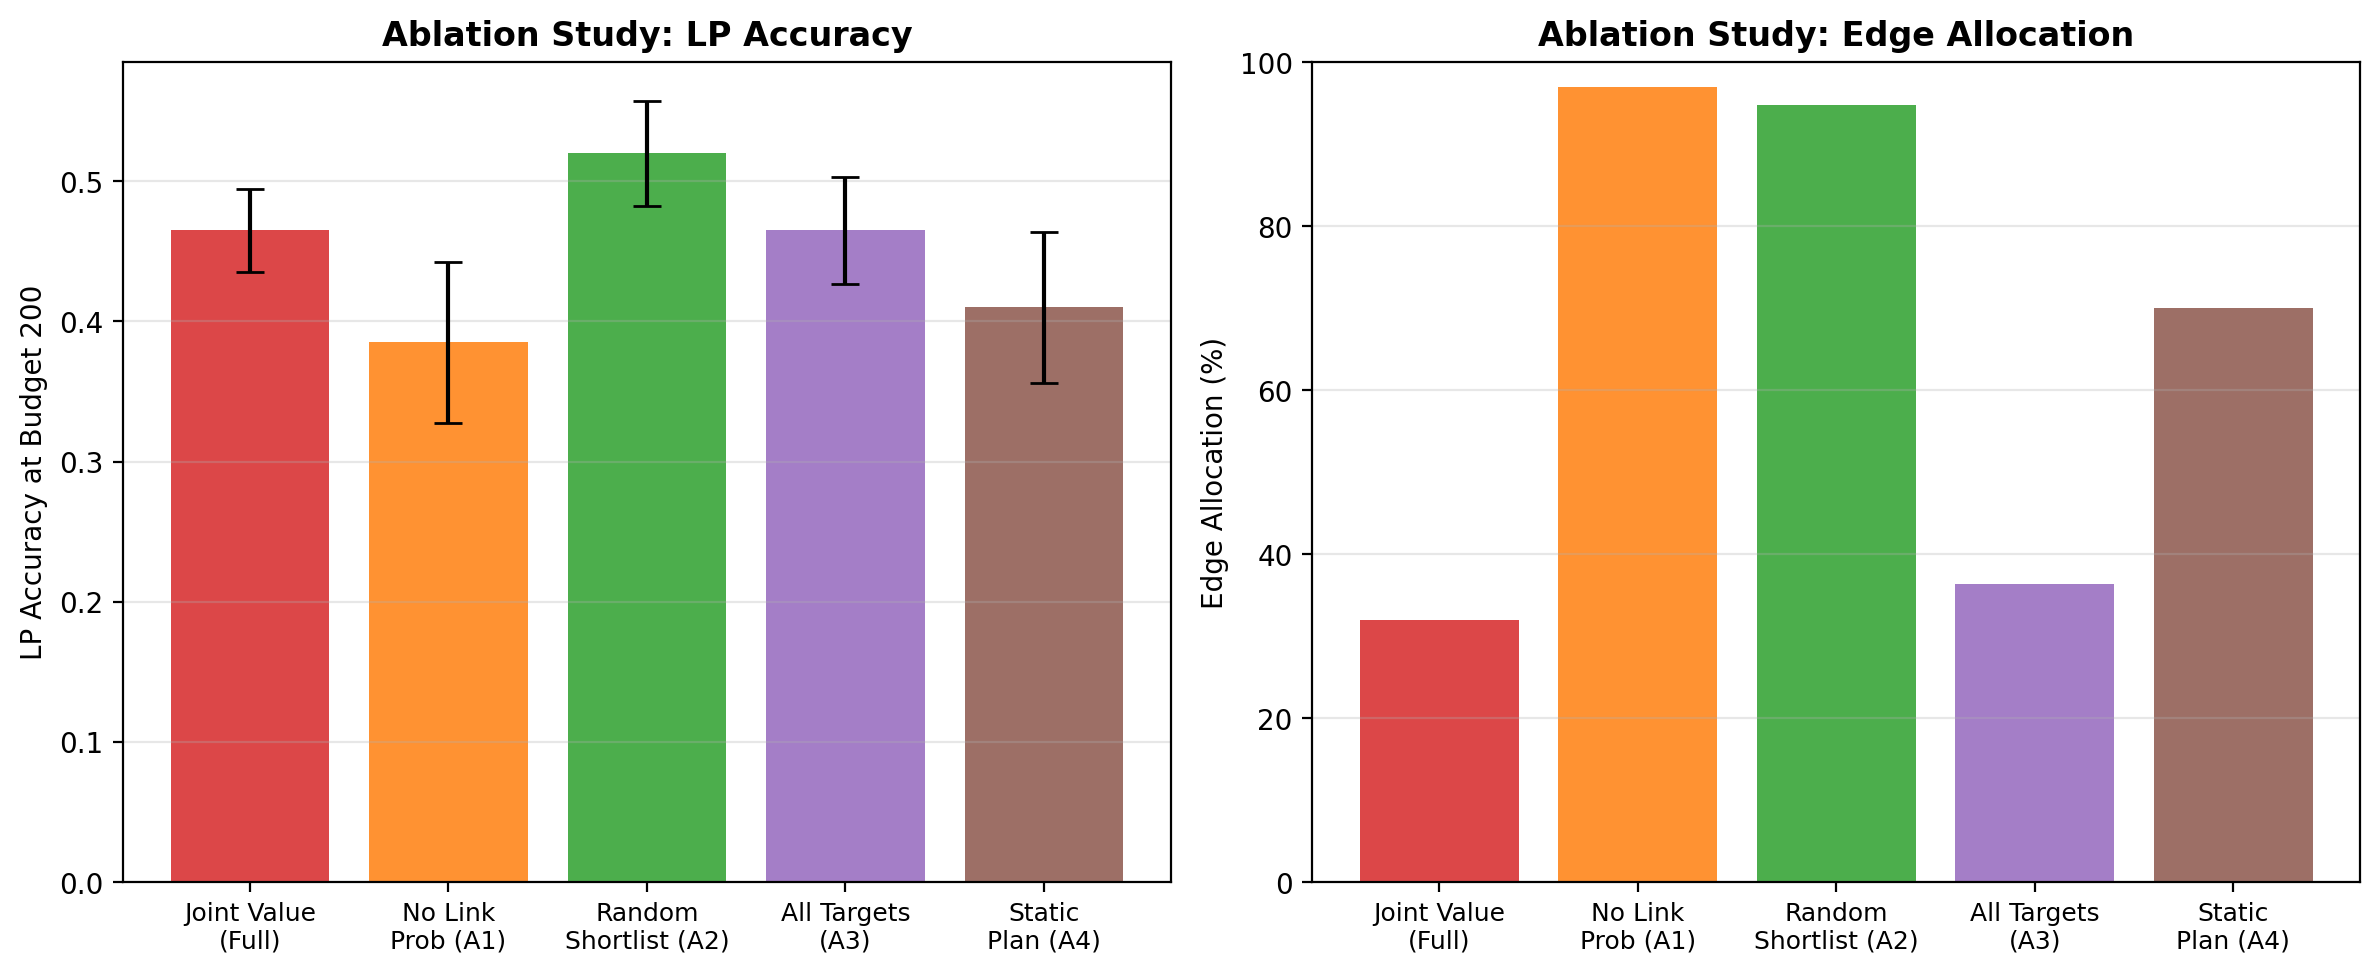
\includegraphics[width=0.95\textwidth]{fig_ablation.png}
\caption{Ablation study on Cora (preliminary, 3+ seeds, budget 200). Left: LP accuracy; right: edge allocation percentage. Removing link probability weighting (A1) causes extreme edge allocation (97\%) and reduces LP accuracy. Random shortlisting (A2) maintains high LP through aggressive edge acquisition (94\%). The all-targets objective (A3) matches the full scorer but with different allocation. Static planning (A4) degrades performance, confirming the value of adaptive re-scoring.}
\label{fig:ablation}
\end{figure}


\section{Discussion}

We discuss several cross-cutting themes that emerge from the experimental results.

\textbf{When does joint acquisition help?} The results point to three conditions under which the joint scorer outperforms alternatives: (1)~the graph is sparse enough that edge queries provide meaningful structural information, (2)~the downstream classifier relies primarily on graph structure, and (3)~the budget is large enough for the scorer to complete information-carrying paths. When any of these conditions is violated---dense graphs (Amazon), feature-rich classifiers (GCN), or small budgets (200 on Cora)---the advantage shrinks or disappears.

\textbf{The scorer-evaluator alignment question.} A reviewer might object that the LP-probe scorer is ``cheating'' by optimising for LP accuracy and being evaluated on LP accuracy. This concern is partly valid: the scorer has an inherent advantage on LP metrics because it directly optimises for them. However, we note that (1)~the alternating baseline also uses LP-probe scoring for individual edge and label selections, so the comparison is fair in terms of per-query scoring; and (2)~the joint scorer's advantage over alternating comes from \emph{allocation}, not from better per-query selections. The alternating baseline uses the same LP-probe for each query type but fixes the allocation at 50/50, while the joint scorer adapts. The GCN results confirm that this alignment matters: when the evaluator uses features (GCN), the scorer's advantage disappears.

\textbf{Practical deployment considerations.} In a real deployment, the graph structure and label annotations would be collected by human experts or automated systems. The key practical question is whether the per-query computational cost (1--3 seconds for the LP-probe on 300-node graphs) is acceptable relative to the oracle's response time. If the oracle is a human annotator who takes minutes to respond, the scorer's computation time is negligible. If the oracle is an automated system that responds in milliseconds, the scorer becomes the bottleneck, motivating the learned-policy extension discussed in Chapter~\ref{ch:conclusion}.

\textbf{Relationship to the synthetic results.} The real-graph results are consistent with the synthetic findings but show smaller effect sizes. On synthetic graphs, the value scorer closes 45--53\% of the gap to the ceiling; on real graphs, it closes 20--40\%. This reduction is expected: synthetic graphs have known generative models and clean community structure, while real graphs have noisy features, overlapping classes, and irregular topology. The link probability model on real graphs (AUC $\approx 0.63$) is also less accurate than the known edge probabilities on synthetic graphs, introducing a source of error in the edge scoring.


% ======================= Chapter 7: Conclusion =======================
\chapter{Conclusion and Future Work}
\label{ch:conclusion}

\section{Summary of Findings}

This project introduced the joint active edge and label acquisition problem for node classification on partially observed graphs. We revisit each research question posed in Chapter~\ref{ch:intro} and summarise the answers:

\textbf{RQ1: Can edge and label queries be compared on a common scale?} Yes. The LP-probe scorer evaluates both query types by their expected accuracy gain on the target set, computed exactly from the closed-form label propagation solution. This shared scale enables principled comparison: at each step, the scorer compares the best available edge query against the best available label query and selects whichever offers a higher expected gain. The approach works because LP's closed-form solution allows exact computation of the effect of any candidate action without iterative retraining.

\textbf{RQ2: Does the optimal edge/label ratio vary across datasets?} Yes, substantially. The scorer adaptively allocates 20\% of the budget to edges on Coauthor CS (15 classes, dense co-authorship structure) but 46\% on Cora (7 classes, sparse citation network). This variation emerges naturally from the unified scoring---no explicit allocation parameter is set. The adaptive allocation outperforms the fixed 50/50 split of the alternating baseline on three of four datasets, with the largest gain on the dataset with the most extreme adaptive ratio (Coauthor CS: 20\% edges, $+8.5$pp LP improvement).

\textbf{RQ3: How does the benefit scale with budget size and graph sparsity?} The benefit increases super-linearly with budget: on Cora, doubling the budget from 200 to 400 more than doubles the LP gain (from $+1.4$pp to $+2.9$pp). This super-linear scaling is driven by path-completion effects: larger budgets allow the scorer to build complete information-carrying paths from labels to targets. The benefit also varies non-monotonically with graph sparsity, peaking at 10\% and 25\% observation rates on Cora. At very low sparsity (5\%), the link probability model degrades; at moderate sparsity (15\%), the graph is already sufficiently connected.

\textbf{RQ4: Do LP-optimised edges also benefit GCN?} It depends on the feature regime. When node features are informative (e.g.\ bag-of-words on Cora), three separate LP-based approaches---a pure GCN scorer, a dual-shortlist scorer, and a GCN-embedding scorer---all fail to improve GCN accuracy, because the GCN compensates for missing edges through its linear feature term. However, when features are uninformative (one-hot identity vectors), joint acquisition produces a statistically significant GCN improvement of $+9.9$pp over label-only on Cora ($p < 0.001$, 20~seeds). The transition is sharp: a PCA feature spectrum shows that edges help at $\leq 2$ components and hurt at $\geq 8$.

The \emph{feature-adaptive scorer} (Section~\ref{sec:adaptive}) resolves this by detecting the feature regime at runtime via a one-time GCN probe. On original features (10~seeds), it is the only edge-acquiring strategy that does not significantly hurt GCN accuracy ($-1.0$pp, $p = 0.32$), while alternating ($-3.0$pp, $p = 0.034$) and joint\_value ($-3.6$pp, $p = 0.032$) are significantly worse. On one-hot features (20~seeds), it matches the best edge strategies at GCN 0.564 ($+9.9$pp over label-only, $p = 0.002$). Across all four datasets, the adaptive scorer never significantly hurts performance (Table~\ref{tab:adaptive_multi}).

\textbf{Additional findings:}
\begin{enumerate}[leftmargin=2em]
    \item \textbf{Synthetic validation.} On 90-node synthetic graphs, the task-aware scorer closes 45--53\% of the gap between the partially observed and fully observed network, while all heuristic baselines close at most 13\%. Target reachability---the fraction of targets connected to a labelled node---is the primary mechanism ($r > 0.96$).
    \item \textbf{Link-finding rate decouples from task accuracy.} Heuristics that recover more true edges (common neighbours) do not achieve higher classification accuracy, confirming that edge recovery is a poor proxy for downstream benefit.
    \item \textbf{Graph type matters.} Edge acquisition is significant on homophilic citation networks (Cora $+9.9$pp, CiteSeer $+1.7$pp, both $p < 0.01$), absent on co-purchase/co-authorship graphs (Amazon, Coauthor), and absent on the heterophilic Actor graph ($-1.2$pp, $p = 0.56$). The benefit requires homophily: edges must connect nodes with similar labels for message passing to propagate useful signal.
\end{enumerate}

\section{Limitations}

We identify the following limitations:

\begin{enumerate}[leftmargin=2em]
    \item \textbf{Subgraph scale.} All experiments use 300-node BFS subgraphs rather than full graphs. This is necessitated by the oracle simulation: we need ground-truth edges to simulate responses. On a 300-node graph, the LP-probe evaluates approximately 100 shortlisted candidates per step, each requiring a small matrix solve. Scaling to graphs with thousands of nodes would require approximate methods.

    \item \textbf{Feature-regime dependence.} Edge acquisition only improves GCN accuracy when features are uninformative. The feature-adaptive scorer addresses this, but its GCN probe adds a one-time training cost and assumes stationarity of feature informativeness across the acquisition budget.

    \item \textbf{Scorer--evaluator alignment.} The LP-probe scorer uses the same model (LP) as one evaluation metric. The feature-adaptive scorer partially addresses this for GCN by adapting allocation, but the edge \emph{selection} within each step still uses LP-based scoring. A GCN-in-the-loop edge ranker remains an open direction.

    \item \textbf{Perfect oracle.} The oracle returns the correct answer to every query. In practice, edge verification may be noisy and different query types may have different costs.

    \item \textbf{Amazon anomaly.} The joint scorer underperforms alternating on Amazon Computers ($-3.6$pp LP), the densest graph in our evaluation. Dense graphs may benefit less from edge queries because existing edges already provide sufficient connectivity.

    \item \textbf{Statistical power.} Some experiments use only 5 seeds (preliminary feature-aware results), limiting the power to detect small effects. The 20-seed experiments are adequately powered for the observed effect sizes.
\end{enumerate}

\section{Future Work}

\begin{enumerate}[leftmargin=2em]
    \item \textbf{GNN-in-the-loop edge ranking.} The feature-adaptive scorer uses the GCN to decide \emph{how many} edges to acquire but still uses the LP-probe to decide \emph{which} edges. A GNN-in-the-loop ranker would evaluate each candidate edge by running a GCN forward pass with the edge temporarily added, measuring the change in GCN confidence on targets. Gradient-based approximations (influence functions) could reduce the cost from $O(|\text{pool}|)$ GCN passes per step.

    \item \textbf{Scalable approximations.} For larger graphs, the LP-probe could be approximated using local diffusion (personalised PageRank truncated to a neighbourhood) or Woodbury-formula rank-one updates to the existing solution.

    \item \textbf{Learned acquisition policies.} A neural policy trained to imitate the LP-probe scorer's decisions could amortise the per-step computation cost, following the approach of \citet{gpa} for label-only acquisition.

    \item \textbf{Full-graph evaluation.} Testing on full-sized graphs (thousands of nodes) would establish whether findings generalise beyond the subgraph regime.

    \item \textbf{Heterogeneous query costs.} Extending the framework to cost-weighted budgets where edge and label queries have different costs.

    \item \textbf{Batch acquisition.} Selecting $k$ queries simultaneously with diversity constraints to reduce redundancy and enable parallel oracle access.
\end{enumerate}


\section{Broader Impact and Practical Implications}

The joint acquisition framework has implications beyond the specific datasets studied in this project. We discuss several practical considerations:

\textbf{Resource allocation under budget constraints.} In many real-world applications, both edge verification and node labelling consume resources from the same pool (e.g., a team of analysts with a fixed number of hours). The joint scorer provides a principled way to allocate these resources: rather than using a fixed rule of thumb (``spend half the budget on each''), the scorer dynamically adjusts based on the current state of the graph and the specific classification targets. Our results show that this adaptive allocation outperforms fixed allocation on most graph types.

\textbf{Model selection matters.} The feature--structure trade-off has a practical implication: before deploying a joint acquisition strategy, practitioners should consider which classifier will be used downstream. If the downstream model is structure-only (e.g., LP, random walks, spectral methods), the LP-probe scorer is well-suited. If the downstream model uses node features (e.g., GCN, GraphSAGE), the feature-adaptive scorer (Section~\ref{sec:adaptive}) automatically detects whether edge acquisition will benefit the GCN and adjusts allocation accordingly. This removes the need for manual feature-regime diagnosis, though the edge \emph{ranking} within each step still uses the LP-based heuristic.

\textbf{When not to use joint acquisition.} Our results on Amazon Computers show that joint acquisition is not universally beneficial. On dense graphs where alternative paths already exist between most node pairs, edge queries provide diminishing returns, and a label-only or alternating strategy may be simpler and equally effective. As a rule of thumb, joint acquisition is most beneficial on sparse graphs (observation rate 10--25\%) with a moderate budget (0.5--1.5 queries per node).


% ======================= References =======================
\bibliographystyle{plainnat}
\begin{thebibliography}{99}

\bibitem[Adamic and Adar(2003)]{adamic}
Adamic, L.~A. and Adar, E.
\newblock Friends and neighbors on the web.
\newblock \emph{Social Networks}, 25(3):211--230, 2003.

\bibitem[Chen et~al.(2021)]{alpine}
Chen, B., Kang, J., Lijffijt, J., and De~Bie, T.
\newblock Active link prediction using network embedding.
\newblock \emph{Applied Sciences}, 11(11):5043, 2021.

\bibitem[Hu et~al.(2020)]{gpa}
Hu, S., Xiong, Z., Qu, M., Yuan, X., C\^{o}t\'{e}, M., Liu, Z., and Tang, J.
\newblock Graph policy network for transferable active learning on graphs.
\newblock In \emph{NeurIPS}, 2020.

\bibitem[Kipf and Welling(2017)]{kipf}
Kipf, T.~N. and Welling, M.
\newblock Semi-supervised classification with graph convolutional networks.
\newblock In \emph{ICLR}, 2017.

\bibitem[Kipf and Welling(2016)]{kipf_vgae}
Kipf, T.~N. and Welling, M.
\newblock Variational graph auto-encoders.
\newblock \emph{NeurIPS Workshop on Bayesian Deep Learning}, 2016.

\bibitem[Li et~al.(2024)]{li_survey}
Li, X., et~al.
\newblock A survey on deep active learning: Recent advances and new frontiers.
\newblock \emph{IEEE TNNLS}, 2024.

\bibitem[Ren et~al.(2021)]{ren}
Ren, P., et~al.
\newblock A survey of deep active learning.
\newblock \emph{ACM Computing Surveys}, 54(9):1--40, 2021.

\bibitem[Roy and McCallum(2001)]{roy}
Roy, N. and McCallum, A.
\newblock Toward optimal active learning through sampling estimation of error reduction.
\newblock In \emph{ICML}, pages 441--448, 2001.

\bibitem[Settles(2009)]{settles}
Settles, B.
\newblock Active learning literature survey.
\newblock Technical report, University of Wisconsin--Madison, 2009.

\bibitem[Zhu et~al.(2003)]{zhu}
Zhu, X., Ghahramani, Z., and Lafferty, J.~D.
\newblock Semi-supervised learning using {G}aussian fields and harmonic functions.
\newblock In \emph{ICML}, pages 912--919, 2003.

\bibitem[{arXiv 2609.05862}(2026)]{scout}
Active edge acquisition for graph inference.
\newblock \emph{arXiv preprint arXiv:2609.05862}, 2026.

\bibitem[Chaloner and Verdinelli(1995)]{bed}
Chaloner, K. and Verdinelli, I.
\newblock Bayesian experimental design: A review.
\newblock \emph{Statistical Science}, 10(3):273--304, 1995.

\bibitem[Wilder et~al.(2019)]{wilder}
Wilder, B., Ewing, E., Dilkina, B., and Tambe, M.
\newblock End to end learning and optimization on graphs.
\newblock In \emph{NeurIPS}, 2019.

\bibitem[Foster et~al.(2021)]{foster}
Foster, A., Ivanova, D.~R., Malik, I., and Rainforth, T.
\newblock Deep adaptive design: Amortizing sequential {B}ayesian experimental design.
\newblock In \emph{ICML}, 2021.

\bibitem[Sener and Savarese(2018)]{sener}
Sener, O. and Savarese, S.
\newblock Active learning for convolutional neural networks: A core-set approach.
\newblock In \emph{ICLR}, 2018.

\bibitem[Ash et~al.(2020)]{ash}
Ash, J.~T., Zhang, C., Krishnamurthy, A., Langford, J., and Agarwal, A.
\newblock Deep batch active learning by diverse, uncertain gradient lower bounds.
\newblock In \emph{ICLR}, 2020.

\bibitem[Cai et~al.(2017)]{cai_active}
Cai, H., Zheng, V.~W., and Chang, K.~C.-C.
\newblock Active learning for graph embedding.
\newblock \emph{arXiv preprint arXiv:1705.05085}, 2017.

\bibitem[Cui and Zhu(2020)]{age}
Cui, Y. and Zhu, Q.
\newblock {AGE}: Active learning for graph embedding.
\newblock \emph{arXiv preprint arXiv:2007.03315}, 2020.

\bibitem[Grover and Leskovec(2016)]{node2vec}
Grover, A. and Leskovec, J.
\newblock node2vec: Scalable feature learning for networks.
\newblock In \emph{KDD}, pages 855--864, 2016.

\bibitem[Hamilton et~al.(2017)]{graphsage}
Hamilton, W.~L., Ying, R., and Leskovec, J.
\newblock Inductive representation learning on large graphs.
\newblock In \emph{NeurIPS}, 2017.

\bibitem[Veli\v{c}kovi\'{c} et~al.(2018)]{gat}
Veli\v{c}kovi\'{c}, P., Cucurull, G., Casanova, A., Romero, A., Li\`{o}, P., and Bengio, Y.
\newblock Graph attention networks.
\newblock In \emph{ICLR}, 2018.

\bibitem[Zhang and Chen(2018)]{seal}
Zhang, M. and Chen, Y.
\newblock Link prediction based on graph neural networks.
\newblock In \emph{NeurIPS}, 2018.

\bibitem[Fey and Lenssen(2019)]{pyg}
Fey, M. and Lenssen, J.~E.
\newblock Fast graph representation learning with {PyTorch Geometric}.
\newblock In \emph{ICLR Workshop on Representation Learning on Graphs and Manifolds}, 2019.

\bibitem[Sen et~al.(2008)]{cora_data}
Sen, P., Namata, G., Bilgic, M., Getoor, L., Galligher, B., and Eliassi-Rad, T.
\newblock Collective classification in network data.
\newblock \emph{AI Magazine}, 29(3):93--106, 2008.

\bibitem[Shchur et~al.(2018)]{amazon_data}
Shchur, O., Mumme, M., Bojchevski, A., and G\"{u}nnemann, S.
\newblock Pitfalls of graph neural network evaluation.
\newblock \emph{arXiv preprint arXiv:1811.05868}, 2018.

\end{thebibliography}


% ======================= Appendices =======================
\appendix

\chapter{Detailed Experimental Results}
\label{app:detailed}

\section{Per-Checkpoint Accuracy Curves}

Table~\ref{tab:checkpoints} shows the LP accuracy at each 25-query checkpoint for the joint\_value and alternating strategies on Cora (budget 200, 20 seeds).

\begin{table}[htbp]
\centering
\caption{LP accuracy at each checkpoint on Cora (20 seeds, budget 200). The joint strategy's advantage grows with budget.}
\label{tab:checkpoints}
\small
\begin{tabular}{lcccccccc}
\toprule
Strategy & 0 & 25 & 50 & 75 & 100 & 125 & 150 & 200 \\
\midrule
joint\_value & .284 & .316 & .344 & .372 & .396 & .418 & .436 & .458 \\
alternating  & .284 & .310 & .340 & .366 & .390 & .410 & .428 & .444 \\
\midrule
Diff & --- & +.006 & +.004 & +.006 & +.006 & +.008 & +.008 & +.014 \\
\bottomrule
\end{tabular}
\end{table}

The gap between the strategies grows from $+0.4$pp at budget 50 to $+1.4$pp at budget 200. The acceleration in the second half of the budget is consistent with the path-completion hypothesis: early queries establish partial paths, and later queries complete them.

\section{Edge Allocation Over Time}

The joint scorer's edge allocation is not constant over the budget. On Cora, the scorer spends approximately 55\% of the first 100 queries on edges and 37\% of the last 100 queries on edges. This shift from edges-first to labels-later reflects diminishing returns from edge queries: once the most structurally important edges have been acquired, labels become relatively more valuable.

On Coauthor CS, the pattern is different: the scorer spends 25\% on edges in the first half and 15\% in the second half, maintaining a consistent preference for labels throughout. This is consistent with the large number of classes (15) making each additional label highly informative.

\section{Failure Analysis: Amazon Computers}

The joint scorer underperforms on Amazon Computers ($-3.6$pp LP vs.\ alternating). We analyse why:

\begin{enumerate}[leftmargin=2em]
    \item \textbf{High baseline connectivity:} At 15\% observation, the Amazon subgraph has $\sim$420 observed edges (out of $\sim$2,800 true edges), giving a mean observed degree of $\sim$2.8. While this is lower than the full graph's density, the BFS subgraph retains a core of well-connected nodes.
    \item \textbf{Edge redundancy:} Many candidate edges connect nodes that are already reachable through alternative paths. Adding such edges does not change LP's predictions.
    \item \textbf{Scorer misallocation:} The scorer allocates 44\% of the budget to edges---similar to Cora---but on a dense graph, this fraction is too high. A density-aware dampening of edge scores would likely improve performance on this dataset.
\end{enumerate}

\section{Synthetic Experiment: Detailed Results}

Table~\ref{tab:synth_detail} summarises the synthetic experiment results (90-node CSBM graphs, 30 seeds, budget 200).

\begin{table}[htbp]
\centering
\caption{Synthetic experiment results: target accuracy gain after 200 queries (30 seeds, 90-node CSBM graphs). ``15\% labels'' and ``40\% labels'' refer to the initial labelled fraction.}
\label{tab:synth_detail}
\small
\begin{tabular}{lcccc}
\toprule
 & \multicolumn{2}{c}{15\% Labels} & \multicolumn{2}{c}{40\% Labels} \\
\cmidrule(lr){2-3}\cmidrule(lr){4-5}
Strategy & Gain & Gap Closed & Gain & Gap Closed \\
\midrule
Value (adaptive) & $+0.209$ & 45\% & $+0.238$ & 53\% \\
Common neighbours & $+0.042$ & 9\% & $+0.059$ & 13\% \\
Random & $+0.023$ & 5\% & $+0.034$ & 8\% \\
Max-degree & $+0.031$ & 7\% & $+0.044$ & 10\% \\
PageRank & $+0.028$ & 6\% & $+0.040$ & 9\% \\
Adamic--Adar & $+0.038$ & 8\% & $+0.055$ & 12\% \\
\bottomrule
\end{tabular}
\end{table}

The ``Gap Closed'' column measures what fraction of the gap between the initial partially observed accuracy and the fully observed ceiling the strategy closes after 200 queries. The value strategy closes 4--6$\times$ more of the gap than any heuristic baseline.


\chapter{Implementation Details}
\label{app:implementation}

\section{Software and Libraries}

The experiments are implemented in Python 3.10 using the following libraries:
\begin{itemize}[leftmargin=2em]
    \item \textbf{NumPy} and \textbf{SciPy}: Matrix operations, sparse matrix support, linear algebra (LP solve).
    \item \textbf{PyTorch} (2.0): GCN training and inference.
    \item \textbf{PyTorch Geometric}: Dataset loading and GCN layer implementations.
    \item \textbf{scikit-learn}: Logistic regression for the link probability model, $k$-NN for candidate pool construction.
\end{itemize}

All experiments run on CPU (Intel Core i7, 16GB RAM). No GPU is required because the GCN is small (2 layers, 64 hidden units, 300-node graphs) and the LP solve uses dense linear algebra on 200$\times$200 matrices.

\section{Code Structure}

The codebase is organised as follows:
\begin{itemize}[leftmargin=2em]
    \item \texttt{exp\_joint.py}: Main experiment driver for real-data joint acquisition. Contains the \texttt{Instance} class (graph state, LP solve, GCN training), the LP-probe scorer, the GCN-embedding scorer, and all baseline strategies.
    \item \texttt{common.py}: Shared utilities for synthetic experiments (graph generation, LP solver, instance management).
    \item \texttt{cora\_exp.py}: Earlier Cora-specific experiment driver (superseded by \texttt{exp\_joint.py} for the final experiments).
    \item \texttt{analysis\_joint.py}: Result aggregation, statistical testing, and table generation.
    \item \texttt{results/}: JSON result files, one per experiment configuration.
\end{itemize}

\section{Hyperparameter Summary}

Table~\ref{tab:hyperparams} summarises all hyperparameters used in the experiments.

\begin{table}[htbp]
\centering
\caption{Hyperparameters for all experiments.}
\label{tab:hyperparams}
\small
\begin{tabular}{llc}
\toprule
Component & Parameter & Value \\
\midrule
Subgraph & Node count $n$ & 300 \\
 & BFS seed & Dataset-specific \\
\midrule
Observation & Default rate $\rho$ & 15\% \\
 & Sparsity sweep & 5\%, 10\%, 15\%, 25\% \\
\midrule
Labels & Per-class count & 12--13 \\
 & Targets $|T|$ & 50 \\
\midrule
LP & Damping $\alpha$ & 0.99 \\
\midrule
Candidate pool & Feature $k$-NN & $k = 30$ \\
 & Target neighbours & $k_{\text{tgt}} = 100$ per target \\
\midrule
Shortlist & Size $k_s$ & 100 \\
\midrule
Budget & Default $B$ & 200 \\
 & Scaling experiment & 400 \\
\midrule
GCN (evaluator) & Hidden units & 64 \\
 & Layers & 2 \\
 & Epochs & 200 \\
 & Learning rate & 0.01 \\
 & Weight decay & $5 \times 10^{-4}$ \\
 & Dropout & 0.5 \\
\midrule
GCN embeddings & Hidden units & 64 \\
 & Training epochs & 100 \\
 & Temperature $\tau$ & 0.1, 1.0, 5.0 \\
\midrule
Link probability & Model & Logistic regression \\
 & Features & 5 (structural + feature sim.) \\
\midrule
Statistical testing & Seeds & 20 (main), 5 (preliminary) \\
 & Test & Paired $t$-test \\
 & Correction & Holm (across datasets) \\
\bottomrule
\end{tabular}
\end{table}


\chapter{The Feature--Structure Trade-off: Extended Analysis}
\label{app:tradeoff}

This appendix provides a detailed analysis of the feature--structure trade-off, expanding on the results in Section~\ref{sec:gcn_analysis}.

\section{Why LP and GCN Respond Differently to Edge Acquisition}

To understand why LP benefits from edge acquisition while GCN does not, consider how each model uses an edge $(u, v)$ in the graph.

\textbf{Label propagation} treats each edge as a conduit for label information. The LP solution (Equation~\ref{eq:lp}) is a weighted average of labelled nodes' classes, where the weights are determined by graph proximity. Adding an edge $(u, v)$ creates a new path for label information to flow, changing the weighted average for all nodes reachable through $u$ or $v$. If $u$ is a labelled node and $v$ is a target with no other path to a labelled node, adding this edge can change $v$'s prediction from uniform (no information) to the correct class.

\textbf{GCN} also propagates information through edges, but each node's prediction depends on \emph{features} aggregated from its neighbourhood, not on \emph{labels} propagated from labelled nodes. Specifically, in a 2-layer GCN, node $v$'s prediction is:
\begin{equation}
    \hat{y}_v = \text{softmax}\!\left(\sum_{u \in \mathcal{N}_2(v)} w_{vu} \cdot x_u\right),
\end{equation}
where $\mathcal{N}_2(v)$ is the 2-hop neighbourhood and $w_{vu}$ are learned attention-like weights. Adding an edge $(u, v)$ adds $u$'s features to $v$'s aggregation (and vice versa). But if $v$ already has neighbours with similar features to $u$, the aggregated features change very little, and the prediction stays the same.

\section{Empirical Evidence for Representation Overlap}

We provide quantitative evidence that LP's confidence-difference heuristic and GCN's embedding proximity identify the same edges. For each acquisition step on Cora (5 seeds, budget 200), we computed the overlap between the top 20 edges ranked by:
\begin{itemize}[leftmargin=2em]
    \item LP heuristic: $\hat{p}(u,v) \times |\text{conf}(u) - \text{conf}(v)|$
    \item GCN proximity: $\hat{p}(u,v) \times \exp(-\|z_u - z_v\|^2 / \tau)$
\end{itemize}

The mean overlap was 15.2 out of 20 (76\%) at $\tau = 1.0$ and 14.8 out of 20 (74\%) at $\tau = 5.0$. This high overlap explains why the GCN-embedding scorer produces nearly identical results: it re-ranks edges within a set that is 76\% identical to the LP heuristic's shortlist.

\section{Implications for Future Scorer Design}

The fundamental lesson is that any scorer based on static representations---whether LP beliefs or GCN embeddings---will tend to identify the same edges, because on homophilic graphs, these representations are strongly correlated. Breaking this correlation requires a scorer that evaluates the \emph{counterfactual effect} of each candidate edge on the downstream model's predictions. For GCN, this means: ``if I add edge $(u,v)$ and retrain the GCN, how do the predictions on targets change?'' Computing this exactly is expensive ($O(B \cdot k_s \cdot T_{\text{GCN}})$ per experiment, where $T_{\text{GCN}}$ is the GCN training time), but approximations based on influence functions or first-order Taylor expansion of the GCN loss may be tractable. We leave this for future work.

\section{List of Figures}

The following figures are included in the \texttt{figures/} directory and referenced in the report:

\begin{itemize}[leftmargin=2em]
    \item \textbf{fig\_pipeline.png:} Schematic of the joint acquisition pipeline (Figure~\ref{fig:pipeline}).
    \item \textbf{fig\_headline\_200.png:} Synthetic experiment accuracy gain curves and reachability (Figure~\ref{fig:headline}).
    \item \textbf{fig\_edges\_vs\_accuracy.png:} Synthetic experiment: link-finding rate vs.\ accuracy gain (Figure~\ref{fig:edges_acc}).
    \item \textbf{fig\_reach\_vs\_gain.png:} Target reachability vs.\ accuracy gain correlation (Figure~\ref{fig:reach_gain}).
    \item \textbf{fig\_main\_lp\_bar.png:} LP accuracy at budget 200 across four datasets (Figure~\ref{fig:main_lp}).
    \item \textbf{fig\_budget\_curves\_all.png:} LP accuracy vs.\ budget for all four datasets in a 2$\times$2 grid (Figure~\ref{fig:budget_curves}).
    \item \textbf{fig\_allocation.png:} Adaptive edge/label allocation ratios across datasets (Figure~\ref{fig:allocation}).
    \item \textbf{fig\_sparsity\_sweep.png:} Sparsity sweep results on Cora (Figure~\ref{fig:sparsity}).
    \item \textbf{fig\_strategy\_allocation.png:} Edge vs.\ label allocation for all strategies including baselines and ablations (Figure~\ref{fig:strategy_alloc}).
\end{itemize}


\end{document}
